\documentclass[11pt,a4paper]{article}

% letra manuscrita (Kalam, OFL) en texto y en las letras y numeros de las formulas; compilar con xelatex
\usepackage{fontspec}
\setmainfont{Kalam}[Path=fuentes/, Extension=.ttf, UprightFont=*-Regular, BoldFont=*-Bold, ItalicFont=*-Regular, ItalicFeatures={FakeSlant=0.15}, BoldItalicFont=*-Bold, BoldItalicFeatures={FakeSlant=0.15}]
\newfontfamily\pincel{KaushanScript-Regular.ttf}[Path=fuentes/]
\setsansfont{Kalam}[Path=fuentes/, Extension=.ttf, UprightFont=*-Regular, BoldFont=*-Bold]
\linespread{1.08}
\usepackage[spanish,es-nodecimaldot,es-tabla,es-noshorthands]{babel}
\usepackage[left=2.0cm,right=2.0cm,top=2.0cm,bottom=2.2cm]{geometry}
\usepackage{amsmath,amssymb}
\usepackage{unicode-math}
\setmathfont{latinmodern-math.otf}
\setmathfont{Kalam-Regular.ttf}[Path=fuentes/, range={up/{latin,Latin,num},it/{latin,Latin}->up}]
\setmathfont{Kalam-Bold.ttf}[Path=fuentes/, range={bfup/{latin,Latin,num}->up,bfit/{latin,Latin}->up}]
\usepackage{booktabs,array,tabularx}
\usepackage{graphicx}
\usepackage{xcolor}
\usepackage{framed}
\usepackage{enumitem}
\usepackage{tikz}
\usetikzlibrary{backgrounds}
\usetikzlibrary{arrows.meta,calc}
\usepackage[hidelinks]{hyperref}
\usepackage{caption}
\captionsetup{font=small,labelfont=bf}
\graphicspath{{figs/}{../informe/figs/}}
\setlength{\parskip}{0.45em}
\setlength{\parindent}{0pt}
\setlength{\emergencystretch}{2em}
\numberwithin{equation}{section}

% ---------------------------------------------------------------- aspecto de cuaderno
% hoja cuadriculada gris, titulos en rojo y todo lo demas en tinta negra
\definecolor{rojo}{HTML}{D0101E}        % titulos
\definecolor{tinta}{HTML}{111111}       % texto
\definecolor{lapiz}{HTML}{3A3A3A}       % anotaciones al lado de las cuentas
\definecolor{grilla}{HTML}{C8C8C8}      % cuadricula de la hoja
\colorlet{idea}{tinta}\colorlet{ojo}{tinta}\colorlet{recordar}{tinta}\colorlet{verifico}{tinta}
\color{tinta}

% hoja cuadriculada (5 mm) con marco
\AddToHook{shipout/background}{%
  \put(0,0){\begin{tikzpicture}[remember picture,overlay]
    \draw[grilla, line width=0.3pt, step=5mm] ([shift={(1cm,1cm)}]current page.south west) grid ([shift={(-1cm,-1cm)}]current page.north east);
    \draw[grilla!80!black, line width=0.6pt] ([shift={(1cm,1cm)}]current page.south west) rectangle ([shift={(-1cm,-1cm)}]current page.north east);
  \end{tikzpicture}}}

% titulos en rojo: "N. Tema"; subtitulos en rojo sin numero; pasos en negrilla negra
\makeatletter
\renewcommand\section{\@startsection{section}{1}{\z@}{-3.2ex plus -1ex minus -.2ex}{1.4ex plus .2ex}%
  {\normalfont\pincel\huge\color{rojo}}}
\renewcommand\subsection{\@startsection{subsection}{2}{\z@}{-2.8ex plus -1ex minus -.2ex}{1.0ex plus .2ex}%
  {\normalfont\pincel\LARGE\color{rojo}}}
\renewcommand\subsubsection{\@startsection{subsubsection}{3}{\z@}{-2.2ex plus -1ex minus -.2ex}{0.8ex plus .2ex}%
  {\normalfont\pincel\Large\color{rojo}}}
\renewcommand\paragraph{\@startsection{paragraph}{4}{\z@}{1.4ex plus .4ex}{-0.6em}%
  {\normalfont\color{tinta}}}
\renewcommand\@seccntformat[1]{\ifnum\pdfstrcmp{#1}{section}=0 \csname the#1\endcsname.\ \fi}
% resultado importante: enmarcado en negro
\renewcommand{\boxed}[1]{\fbox{\m@th$\displaystyle #1$}}
\makeatother
\setlength{\arrayrulewidth}{0.9pt}
\setlist[itemize]{label=\textbf{·},leftmargin=1.1em,itemsep=0.1em,topsep=0.2em}

% notas sueltas, como en los apuntes: "· Ojo: ..."
\newenvironment{apunte}[2]{\par\noindent\ignorespaces}{\par}
\newenvironment{idea}{\begin{apunte}{idea}{Idea:}}{\end{apunte}}
\newenvironment{ojo}{\begin{apunte}{ojo}{Ojo:}}{\end{apunte}}
\newenvironment{recordar}{\begin{apunte}{recordar}{Recordar:}}{\end{apunte}}
\newenvironment{verifico}{\begin{apunte}{verifico}{Verifico:}}{\end{apunte}}
% anotacion a mano al lado de un paso: \com{derivando}
% numero de ecuacion en circulo, como en los apuntes
\newcommand{\cnum}[1]{\tikz[baseline=(n.base)]\node[draw,circle,inner sep=1pt,line width=0.6pt](n){\small #1};}
% termino tachado que vale cero
\newcommand{\cancelto}[2]{\tikz[baseline=(t.base)]{\node[inner sep=0pt](t){$\displaystyle #2$};\draw[line width=0.6pt](t.south west)--(t.north east)node[above right,inner sep=0pt]{\scriptsize$#1$};}}
% tabla con la fila de encabezado sombreada en gris
\newsavebox{\cajatabla}
\newcommand{\tablagris}[1]{\sbox{\cajatabla}{#1}\tikz[baseline=(c.base)]{\node[inner sep=0pt](c){\usebox{\cajatabla}};
  \begin{scope}[on background layer]\fill[gray!25]([yshift=-\arrayrulewidth]c.north west) rectangle ([yshift=-1.3\baselineskip-\arrayrulewidth]c.north east);\end{scope}}}
\newcommand{\com}[1]{\qquad\text{\small\color{lapiz}$\leftarrow$ #1}}

\AtBeginDocument{\let\chequeo\checkmark\renewcommand{\checkmark}{\ensuremath{\chequeo}}}  % Kalam no trae el simbolo
\newcommand{\vect}[1]{\symbfit{#1}}
\newcommand{\bm}[1]{\symbfit{#1}}
\newcommand{\T}{^{\top}}
\newcommand{\sk}[1]{\widetilde{#1}}
% Generado por scripts/generar_datos_calculo.py; no editar a mano
\newcommand{\Ts}{2}
\newcommand{\Fmax}{50}
\newcommand{\Fzero}{4.779}
\newcommand{\MzeroMat}{2.7802 & 0 & 0 & 0 & -0.0003 & 0 \\ 0 & 2.7802 & 0 & 0.0003 & 0 & 0 \\ 0 & 0 & 2.7261 & 0 & 0 & 0 \\ 0 & 0.0003 & 0 & 0.0169 & 0 & 0 \\ -0.0003 & 0 & 0 & 0 & 0.0169 & 0 \\ 0 & 0 & 0 & 0 & 0 & 0.0346}
\newcommand{\MzeroEigs}{0.0169,\allowbreak\ 0.0169,\allowbreak\ 0.0346,\allowbreak\ 2.7261,\allowbreak\ 2.7802,\allowbreak\ 2.7802}
\newcommand{\MzeroEigMin}{0.0169}
\newcommand{\AtwoOneMat}{41.00 & 0 & 0 & 0 & -0.23 & 0 \\ 0 & 41.00 & 0 & 0.23 & 0 & 0 \\ 0 & 0 & 5.74 & 0 & 0 & 0 \\ 0 & 37.89 & 0 & 17.22 & 0 & 0 \\ -37.89 & 0 & 0 & 0 & 17.22 & 0 \\ 0 & 0 & 0 & 0 & 0 & 58.09}
\newcommand{\BtwoMat}{-0.097 & -0.097 & 0.097 & 0 & 0 & 0.097 \\ -0.056 & 0.056 & -0.056 & -0.111 & 0.111 & 0.056 \\ 0.349 & 0.349 & 0.349 & 0.349 & 0.349 & 0.349 \\ -4.966 & 4.966 & 6.786 & 1.820 & -1.820 & -6.786 \\ -4.969 & -4.969 & -1.816 & 6.785 & 6.785 & -1.816 \\ -1.080 & 1.080 & -1.080 & 1.080 & -1.080 & 1.080}
\newcommand{\PolosLA}{\pm7.62,\allowbreak\ \pm6.43\ (\times2),\allowbreak\ \pm4.11\ (\times2),\allowbreak\ \pm2.40}
\newcommand{\SigmaMax}{7.62}
\newcommand{\EigAtwoOne}{58.09,\allowbreak\ 41.36,\allowbreak\ 41.36,\allowbreak\ 16.85,\allowbreak\ 16.85,\allowbreak\ 5.74}
\newcommand{\LamEigs}{0.398,\allowbreak\ 0.398,\allowbreak\ 0.502,\allowbreak\ 4.124,\allowbreak\ 10.371,\allowbreak\ 10.371}
\newcommand{\KlEigs}{427.8,\allowbreak\ 427.8,\allowbreak\ 239.6,\allowbreak\ 6.7,\allowbreak\ 6.7,\allowbreak\ 2.9}
\newcommand{\KlMax}{427.8}
\newcommand{\mLeg}{4.3607}
\newcommand{\kLeg}{185.26}
\newcommand{\mEff}{0.8054}
\newcommand{\sigmaLeg}{6.518}
\newcommand{\cLeg}{1.0000850}
\newcommand{\gLeg}{4.5865\times10^{-7}}
\newcommand{\zUnst}{1.013121}
\newcommand{\zSt}{0.987049}
\newcommand{\MxTheta}{2.94\times10^{-4}}
\newcommand{\muMulti}{1.84\times10^{-6}}
\newcommand{\omegaMulti}{1.9986,\allowbreak\ 1.9986,\allowbreak\ 2.0000,\allowbreak\ 2.0000,\allowbreak\ 2.0014,\allowbreak\ 2.0014}
\newcommand{\MdiagPlat}{2 & 2 & 2 & 0.01125 & 0.01125 & 0.0225}
\newcommand{\MdiagPatas}{0.7802 & 0.7802 & 0.7261 & 0.0057 & 0.0057 & 0.0121}
\newcommand{\KpOpt}{4556.7}
\newcommand{\KiOpt}{18445.7}
\newcommand{\KdOpt}{105.43}
\newcommand{\spOpt}{0.759}
\newcommand{\siOpt}{3.074}
\newcommand{\sdOpt}{0.703}
\newcommand{\TiOpt}{0.247}
\newcommand{\TdOpt}{23.14}
\newcommand{\JpidOpt}{4.777}
\newcommand{\alphaD}{0.7261}
\newcommand{\Dcoef}{136.93}
\newcommand{\nTwo}{18992.4}
\newcommand{\nOne}{-36700.1}
\newcommand{\nZero}{17717.8}
\newcommand{\wcPid}{187.9}
\newcommand{\PMPid}{41.6}
\newcommand{\GMPid}{11.1}
\newcommand{\MsPid}{2.15}
\newcommand{\wcHand}{37.6}
\newcommand{\GwcMag}{1.577\times10^{-4}}
\newcommand{\GwcAng}{-182.2}
\newcommand{\CwcMag}{6343}
\newcommand{\CwcAng}{+31.0}
\newcommand{\PMhand}{28.8}
\newcommand{\RouthA}{105.43}
\newcommand{\RouthB}{4371.4}
\newcommand{\RouthC}{18445.7}
\newcommand{\RouthL}{460870}
\newcommand{\RouthR}{80437}
\newcommand{\RootsCont}{-9.77 \pm 28.57j,\allowbreak\ -4.64}
\newcommand{\charPoly}{z^4 -3.7176z^3 +5.1706z^2 -3.1873z +0.7343}
\newcommand{\charRoots}{0.9907,\allowbreak\ 0.9759 \pm 0.0620j,\allowbreak\ 0.7751}
\newcommand{\rhoSiso}{0.9907}
\newcommand{\rhoPid}{0.9945}
\newcommand{\KpBase}{6000}
\newcommand{\KiBase}{6000}
\newcommand{\KdBase}{150}
\newcommand{\alphaOpt}{3.357}
\newcommand{\betaOpt}{0.3525}
\newcommand{\JssOpt}{3.633}
\newcommand{\PoloCtrl}{-85.60 \pm 30.21j}
\newcommand{\PoloObs}{-27.49 \pm 6.34j}
\newcommand{\tsCtrl}{47}
\newcommand{\cofErr}{2.2\times10^{-16}}
\newcommand{\sepErr}{1.3\times10^{-13}}
\newcommand{\normK}{8.75\times10^{4}}
\newcommand{\rhoSS}{0.9696}
\newcommand{\rhoCtrlBlock}{0.9696}
\newcommand{\obsPoleErr}{5.2\times10^{-15}}
\newcommand{\obsZmax}{0.9465}
\newcommand{\LdPos}{0.104 y 0.132}
\newcommand{\LdVel}{1.585 y 2.598}
\newcommand{\aOnda}{2}
\newcommand{\TOnda}{2.5}
\newcommand{\fOnda}{0.2}
\newcommand{\wOnda}{1.2566}
\newcommand{\AOnda}{15}
\newcommand{\rzZero}{15.000}
\newcommand{\kappaOnda}{0.7170}
\newcommand{\EOnda}{6.738\times10^{-3}}
\newcommand{\TPre}{1}
\newcommand{\rzT}{-15.000}
\newcommand{\drzZero}{0.000}
\newcommand{\drzT}{0.000}
\newcommand{\CUnoA}{-10.8273}
\newcommand{\CDosA}{10.8273}
\newcommand{\xZeroA}{0.000}
\newcommand{\xTA}{0.000}
\newcommand{\JA}{393.7}
\newcommand{\CUnoB}{-10.7539}
\newcommand{\CDosB}{-0.0725}
\newcommand{\xZeroB}{0.000}
\newcommand{\xTB}{-10.899}
\newcommand{\JB}{274.9}
\newcommand{\CUnoC}{0.0725}
\newcommand{\CDosC}{10.7539}
\newcommand{\xZeroC}{10.899}
\newcommand{\xTC}{0.000}
\newcommand{\JC}{274.9}
\newcommand{\CUnoD}{0.0000}
\newcommand{\CDosD}{0.0000}
\newcommand{\xZeroD}{10.754}
\newcommand{\xTD}{-10.754}
\newcommand{\JD}{159.2}
\newcommand{\dlEn}{14.26}
\newcommand{\uEnMax}{17.23}
\newcommand{\EEn}{1.980\times10^{-4}}
\newcommand{\aMax}{0.08}
\newcommand{\dlTm}{23.19}
\newcommand{\TMin}{1.077}
\newcommand{\tSw}{0.538}
\newcommand{\vPico}{43.1}
\newcommand{\uBang}{64.4}
\newcommand{\VAFunoMedia}{-306.92}
\newcommand{\FITunoMedia}{-99.7}
\newcommand{\VAFdosMedia}{97.81}
\newcommand{\FITdosMedia}{84.8}
\newcommand{\FITdosMin}{80.2}
\newcommand{\FITanMedia}{84.7}
\newcommand{\IdHval}{0.1}
\newcommand{\aIdMin}{1.91977}
\newcommand{\aIdMax}{1.99607}
\newcommand{\aAn}{2.00301}
\newcommand{\mIdMin}{0.835}
\newcommand{\mIdMax}{0.900}
\newcommand{\mAn}{0.805}
\newcommand{\IdKp}{1500}
\newcommand{\IdKd}{60}
\newcommand{\IdLmin}{275.1}
\newcommand{\IdLmax}{291.7}
\newcommand{\IdSigma}{0.05}
\newcommand{\mIdDirMin}{0.105}
\newcommand{\mIdDirMax}{0.142}
\newcommand{\IdTsId}{10}
\newcommand{\IdFc}{20}
\newcommand{\IdD}{5}
\newcommand{\mErrMax}{12}

\newcommand{\RefSendl}{14.26}
\newcommand{\RefSendld}{40.33}
\newcommand{\RefSenqdd}{119.91}
\newcommand{\RefSenFff}{4.88}
\newcommand{\RefSendv}{0.00}
\newcommand{\RefSendq}{0.00}
\newcommand{\RefSenFreg}{8.84}
\newcommand{\RefSenPidRms}{0.116}
\newcommand{\RefSenPidEmax}{0.37}
\newcommand{\RefSenPidFmax}{20.6}
\newcommand{\RefSenSsRms}{0.124}
\newcommand{\RefSenSsEmax}{0.52}
\newcommand{\RefSenSsFmax}{8.8}
\newcommand{\RefSeisdl}{22.97}
\newcommand{\RefSeisdld}{39.41}
\newcommand{\RefSeisqdd}{60.45}
\newcommand{\RefSeisFff}{7.32}
\newcommand{\RefSeisdv}{0.00}
\newcommand{\RefSeisdq}{0.00}
\newcommand{\RefSeisFreg}{10.36}
\newcommand{\RefSeisPidRms}{1.424}
\newcommand{\RefSeisPidEmax}{11.99}
\newcommand{\RefSeisPidFmax}{50.0}
\newcommand{\RefSeisSsRms}{0.497}
\newcommand{\RefSeisSsEmax}{11.96}
\newcommand{\RefSeisSsFmax}{50.0}
\newcommand{\RefCircdl}{11.81}
\newcommand{\RefCircdld}{29.68}
\newcommand{\RefCircqdd}{94.75}
\newcommand{\RefCircFff}{7.05}
\newcommand{\RefCircdv}{0.00}
\newcommand{\RefCircdq}{0.00}
\newcommand{\RefCircFreg}{10.15}
\newcommand{\RefCircPidRms}{1.740}
\newcommand{\RefCircPidEmax}{14.96}
\newcommand{\RefCircPidFmax}{50.0}
\newcommand{\RefCircSsRms}{0.690}
\newcommand{\RefCircSsEmax}{14.96}
\newcommand{\RefCircSsFmax}{50.0}
\newcommand{\RefFAdl}{4.68}
\newcommand{\RefFAdld}{20.16}
\newcommand{\RefFAqdd}{59.14}
\newcommand{\RefFAFff}{4.81}
\newcommand{\RefFAdv}{21.44}
\newcommand{\RefFAdq}{0.00}
\newcommand{\RefFAFreg}{8.71}
\newcommand{\RefFAPidRms}{0.096}
\newcommand{\RefFAPidEmax}{0.32}
\newcommand{\RefFAPidFmax}{20.6}
\newcommand{\RefFASsRms}{0.071}
\newcommand{\RefFASsEmax}{0.32}
\newcommand{\RefFASsFmax}{8.7}
\newcommand{\RefFBdl}{10.36}
\newcommand{\RefFBdld}{21.09}
\newcommand{\RefFBqdd}{59.15}
\newcommand{\RefFBFff}{4.82}
\newcommand{\RefFBdv}{22.48}
\newcommand{\RefFBdq}{0.00}
\newcommand{\RefFBFreg}{8.73}
\newcommand{\RefFBPidRms}{0.097}
\newcommand{\RefFBPidEmax}{0.32}
\newcommand{\RefFBPidFmax}{20.6}
\newcommand{\RefFBSsRms}{0.073}
\newcommand{\RefFBSsEmax}{0.32}
\newcommand{\RefFBSsFmax}{8.7}
\newcommand{\RefFCdl}{10.36}
\newcommand{\RefFCdld}{21.46}
\newcommand{\RefFCqdd}{59.15}
\newcommand{\RefFCFff}{4.82}
\newcommand{\RefFCdv}{22.35}
\newcommand{\RefFCdq}{0.00}
\newcommand{\RefFCFreg}{8.71}
\newcommand{\RefFCPidRms}{0.097}
\newcommand{\RefFCPidEmax}{0.34}
\newcommand{\RefFCPidFmax}{20.6}
\newcommand{\RefFCSsRms}{0.072}
\newcommand{\RefFCSsEmax}{0.33}
\newcommand{\RefFCSsFmax}{8.7}
\newcommand{\RefFDdl}{10.23}
\newcommand{\RefFDdld}{21.18}
\newcommand{\RefFDqdd}{42.66}
\newcommand{\RefFDFff}{4.82}
\newcommand{\RefFDdv}{22.19}
\newcommand{\RefFDdq}{0.00}
\newcommand{\RefFDFreg}{8.73}
\newcommand{\RefFDPidRms}{0.098}
\newcommand{\RefFDPidEmax}{0.34}
\newcommand{\RefFDPidFmax}{20.6}
\newcommand{\RefFDSsRms}{0.073}
\newcommand{\RefFDSsEmax}{0.31}
\newcommand{\RefFDSsFmax}{8.7}
\newcommand{\RefFijdl}{23.19}
\newcommand{\RefFijdld}{46.31}
\newcommand{\RefFijqdd}{361.37}
\newcommand{\RefFijFff}{7.41}
\newcommand{\RefFijdv}{39.00}
\newcommand{\RefFijdq}{0.00}
\newcommand{\RefFijFreg}{11.53}
\newcommand{\RefFijPidRms}{0.333}
\newcommand{\RefFijPidEmax}{1.41}
\newcommand{\RefFijPidFmax}{21.7}
\newcommand{\RefFijSsRms}{0.086}
\newcommand{\RefFijSsEmax}{0.47}
\newcommand{\RefFijSsFmax}{11.5}
\newcommand{\RefTmindl}{23.19}
\newcommand{\RefTmindld}{42.99}
\newcommand{\RefTminqdd}{68.05}
\newcommand{\RefTminFff}{6.84}
\newcommand{\RefTmindv}{0.00}
\newcommand{\RefTmindq}{0.00}
\newcommand{\RefTminFreg}{10.21}
\newcommand{\RefTminPidRms}{0.306}
\newcommand{\RefTminPidEmax}{0.88}
\newcommand{\RefTminPidFmax}{21.6}
\newcommand{\RefTminSsRms}{0.083}
\newcommand{\RefTminSsEmax}{0.22}
\newcommand{\RefTminSsFmax}{10.2}
\newcommand{\RefCurvadl}{14.26}
\newcommand{\RefCurvadld}{40.33}
\newcommand{\RefCurvaqdd}{119.91}
\newcommand{\RefCurvaFff}{4.88}
\newcommand{\RefCurvadv}{34.59}
\newcommand{\RefCurvadq}{19.24}
\newcommand{\RefCurvaFreg}{50.00}
\newcommand{\RefCurvaPidRms}{0.605}
\newcommand{\RefCurvaPidEmax}{19.05}
\newcommand{\RefCurvaPidFmax}{50.0}
\newcommand{\RefCurvaSsRms}{0.634}
\newcommand{\RefCurvaSsEmax}{19.20}
\newcommand{\RefCurvaSsFmax}{50.0}

\makeatletter\newcommand{\tabinput}[1]{\@@input #1 }\makeatother

\begin{document}

{\color{rojo}\pincel\fontsize{40}{48}\selectfont Plataforma Stewart\par}
\vspace{0.2em}
{\large Cuaderno de cálculos: modelado, trayectorias óptimas y control\par}
{\normalsize Santiago Alejandro Zúñiga Melo --- Estrategias Óptimas de Control, Maestría en Ingeniería Electrónica\par}
\vspace{0.6em}

% =====================================================================================================
\section{Arquitectura}

\noindent
\begin{minipage}[t]{0.46\textwidth}\vspace{0pt}
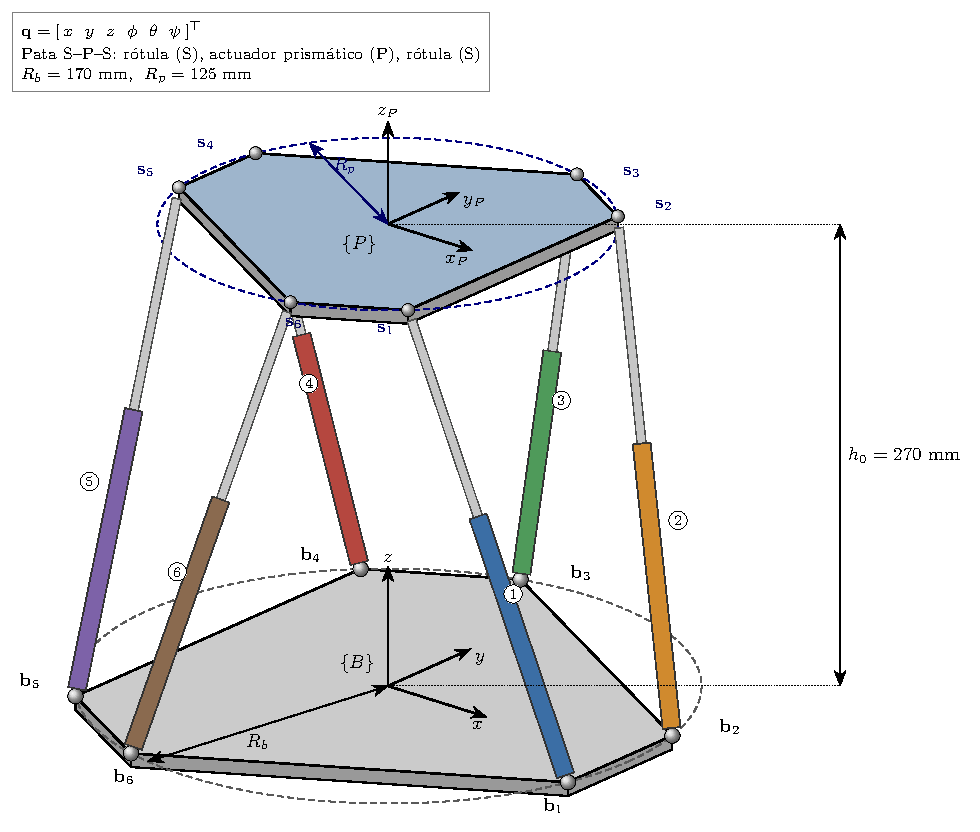
\includegraphics[width=\linewidth]{arquitectura_6sps.pdf}
\end{minipage}\hfill
\begin{minipage}[t]{0.51\textwidth}\vspace{0pt}
El sistema está compuesto por:
\begin{itemize}
\item Base fija $\{B\}$
\item Plataforma móvil $\{P\}$
\item 6 patas con configuración SPS
\end{itemize}
{\small\[
\underbrace{\text{rótula } B_i}_{S} - \underbrace{\text{cilindro}\leftrightarrow\text{pistón}}_{P} - \underbrace{\text{rótula } P_i}_{S}
\]}
La fuerza será descrita por:
\[
\vect F = (F_1, \dots, F_6), \qquad F_i = \text{fuerza axial del actuador } i
\]
\begin{itemize}
\item El sistema cuenta con 6 grados de libertad
\end{itemize}
\[
\vect q = [x\ y\ z\ \phi\ \theta\ \psi]\T :\quad
\begin{array}{l} 3 \text{ movimientos traslacionales} \\ 3 \text{ movimientos rotacionales} \end{array}
\]
\end{minipage}

\subsection{Geometría y parámetros de diseño}

\noindent
\begin{minipage}[t]{0.43\textwidth}\vspace{0pt}
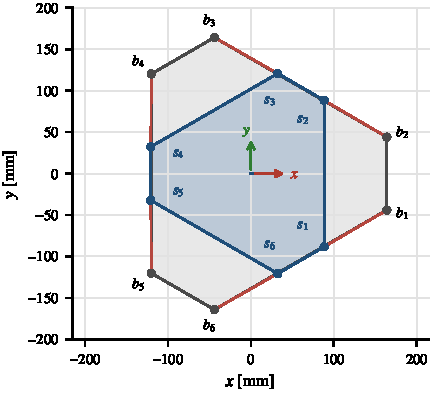
\includegraphics[width=\linewidth]{geometria.pdf}

\smallskip
En reposo: $P_i = \vect s_i + (0,\ 0,\ h_0)$ en $\{B\}$
\end{minipage}\hfill
\begin{minipage}[t]{0.55\textwidth}\vspace{0pt}
\begin{itemize}
\item $\{B\}$: marco de la base, origen en el centro de los anclajes inferiores, eje $z$ arriba.
\item $\{P\}$: marco de la plataforma, origen en su centro; en reposo se encuentra a $h_0 = 270$ mm sobre la base y con los ejes paralelos a $\{B\}$.
\item Anclajes inferiores $B_i$ sobre una circunferencia de radio $R_b = 170$ mm; superiores $P_i$ sobre una de radio $R_p = 125$ mm.
\end{itemize}
\textbf{Coordenadas de los extremos de los actuadores}

\smallskip
{\small\renewcommand{\arraystretch}{1.25}\setlength{\tabcolsep}{4pt}
\begin{tabular}{@{}l|l@{}}
$\vect b_1 = (164.21,\ -44.00,\ 0)$ & $\vect s_1 = (88.39,\ -88.39,\ 0)$ \\
$\vect b_2 = (164.21,\ 44.00,\ 0)$ & $\vect s_2 = (88.39,\ 88.39,\ 0)$ \\
$\vect b_3 = (-44.00,\ 164.21,\ 0)$ & $\vect s_3 = (32.35,\ 120.74,\ 0)$ \\
$\vect b_4 = (-120.21,\ 120.21,\ 0)$ & $\vect s_4 = (-120.74,\ 32.35,\ 0)$ \\
$\vect b_5 = (-120.21,\ -120.21,\ 0)$ & $\vect s_5 = (-120.74,\ -32.35,\ 0)$ \\
$\vect b_6 = (-44.00,\ -164.21,\ 0)$ & $\vect s_6 = (32.35,\ -120.74,\ 0)$
\end{tabular}}
\end{minipage}

\subsubsection{Datos de diseño}

\noindent
{\footnotesize\setlength{\tabcolsep}{4pt}\renewcommand{\arraystretch}{1.3}%
\tablagris{\begin{tabular}{|c|p{3.4cm}|c|c|p{3.6cm}|c|}
\hline
\textbf{Símbolo} & \textbf{Descripción} & \textbf{Valor} & \textbf{Símbolo} & \textbf{Descripción} & \textbf{Valor} \\ \hline
$R_b$ & radio anclajes base & 170 mm & $b_C$ & centro de masa cilindro & 80 mm \\ \hline
$R_p$ & radio anclajes plataforma & 125 mm & $m_S$ & masa pistón & 0.12 kg \\ \hline
$h_0$ & altura nominal & 270 mm & $L_S$ & longitud pistón & 100 mm \\ \hline
$m_P$ & masa plataforma & 2.0 kg & $r_S$ & radio pistón & 6 mm \\ \hline
$r_P$ & radio plataforma & 150 mm & $b_S$ & centro de masa pistón & 50 mm \\ \hline
$m_C$ & masa cilindro & 0.45 kg & $F_{\max}$ & fuerza axial máxima del actuador & $\pm\Fmax$ N \\ \hline
$L_C$ & longitud cilindro & 160 mm & $\ddot l_{\max}$ & aceleración máxima de la pata & 0.08 m/s$^2$ \\ \hline
$r_C$ & radio cilindro & 12 mm & $T_s$ & periodo de muestreo & \Ts{} ms \\ \hline
\end{tabular}}}

% =====================================================================================================
\section{Cinemática}

\subsubsection{2.1.\ Posición y orientación}

Recordemos que la posición y la orientación de $\{P\}$ con respecto a $\{B\}$ está dada por
\[
\vect q = [x\ y\ z\ \phi\ \theta\ \psi]\T ;\quad \vect p = [x\ y\ z]\T ;\quad \boldsymbol\Theta = [\phi\ \theta\ \psi]\T
\]
{\small
\begin{tabular}{@{}l@{\quad}l@{}}
donde: & $\vect q$ vector de coordenadas generalizadas \\
& $\vect p$ es la posición del origen de $\{P\}$ medida en $\{B\}$ \\
& $\boldsymbol\Theta$ agrupa los ángulos de roll ($\phi$), pitch ($\theta$) y yaw ($\psi$)
\end{tabular}}

La orientación de la plataforma la guarda la matriz de rotación $\vect R(\boldsymbol\Theta)$ y esta se encarga de pasar un vector escrito en el marco $\{P\}$ al marco $\{B\}$.

Para el desarrollo del modelo cinemático abordaremos las matrices de rotación; para ello aplicaremos una secuencia de rotación de la forma $Z$-$Y$-$X$:

\subsection{Matrices de rotación}

Consideremos las matrices de rotación elementales
\[
\vect R_x(\phi) = \begin{bmatrix}1 & 0 & 0\\ 0 & \cos\phi & -\sin\phi\\ 0 & \sin\phi & \cos\phi\end{bmatrix}\qquad
\vect R_y(\theta) = \begin{bmatrix}\cos\theta & 0 & \sin\theta\\ 0 & 1 & 0\\ -\sin\theta & 0 & \cos\theta\end{bmatrix}\qquad
\vect R_z(\psi) = \begin{bmatrix}\cos\psi & -\sin\psi & 0\\ \sin\psi & \cos\psi & 0\\ 0 & 0 & 1\end{bmatrix}
\]
Siguiendo el orden de la rotación, entonces
\[
\vect R(\boldsymbol\Theta) = \vect R_z(\psi)\,\vect R_y(\theta)\,\vect R_x(\phi)
\]
{\small\[
\vect R_y(\theta)\vect R_x(\phi) = \begin{bmatrix}\cos\theta & 0 & \sin\theta\\ 0 & 1 & 0\\ -\sin\theta & 0 & \cos\theta\end{bmatrix}
\begin{bmatrix}1 & 0 & 0\\ 0 & \cos\phi & -\sin\phi\\ 0 & \sin\phi & \cos\phi\end{bmatrix}
= \begin{bmatrix}\cos\theta & \sin\theta\sin\phi & \sin\theta\cos\phi\\ 0 & \cos\phi & -\sin\phi\\ -\sin\theta & \cos\theta\sin\phi & \cos\theta\cos\phi\end{bmatrix}
\]}
Ahora
{\small\[
\vect R_z(\psi)\vect R_y(\theta)\vect R_x(\phi) = \begin{bmatrix}\cos\psi & -\sin\psi & 0\\ \sin\psi & \cos\psi & 0\\ 0 & 0 & 1\end{bmatrix}
\begin{bmatrix}\cos\theta & \sin\theta\sin\phi & \sin\theta\cos\phi\\ 0 & \cos\phi & -\sin\phi\\ -\sin\theta & \cos\theta\sin\phi & \cos\theta\cos\phi\end{bmatrix}
\]}
{\small\[
\vect R(\boldsymbol\Theta) = \begin{bmatrix}
\cos\psi\cos\theta & \cos\psi\sin\theta\sin\phi - \sin\psi\cos\phi & \cos\psi\sin\theta\cos\phi + \sin\psi\sin\phi\\
\sin\psi\cos\theta & \sin\psi\sin\theta\sin\phi + \cos\psi\cos\phi & \sin\psi\sin\theta\cos\phi - \cos\psi\sin\phi\\
-\sin\theta & \cos\theta\sin\phi & \cos\theta\cos\phi
\end{bmatrix}
\]}

\subsubsection{2.2\ Cinemática inversa}

Ahora, dado un $\vect q$, necesitamos saber cuánto mide cada pata $l_i(\vect q)$, $i = 1, \dots, 6$, donde $l_i$ es la distancia entre $B_i$ y $P_i$, es decir, la longitud del actuador $i$.

\noindent
\begin{minipage}[t]{0.30\textwidth}\vspace{0pt}
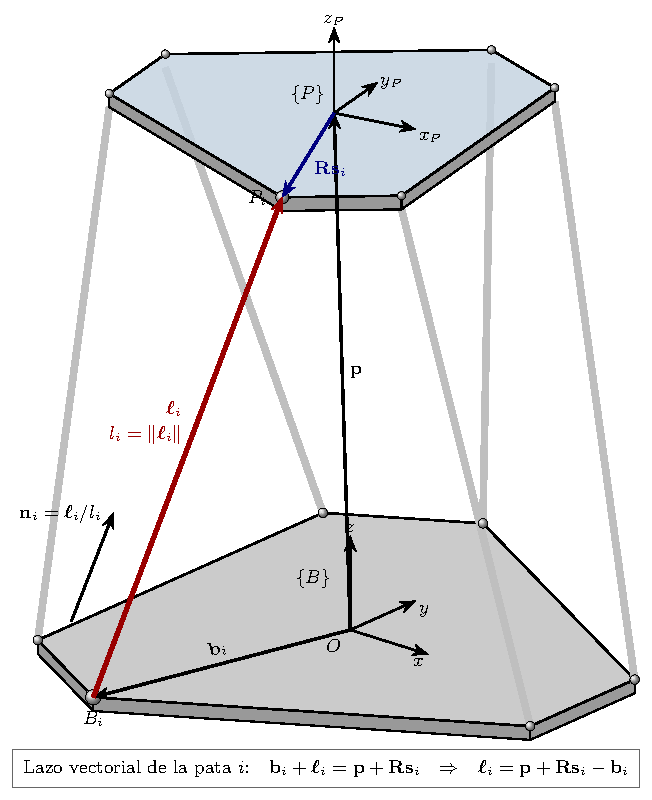
\includegraphics[width=\linewidth]{lazo_vectorial_pata.pdf}
\end{minipage}\hfill
\begin{minipage}[t]{0.68\textwidth}\vspace{0pt}
Para construir un modelo que me permita calcular $l_i$ consideremos un único actuador.

Para esto vamos a considerar los caminos que llegan al punto $P_i$ desde el origen en el marco $\{B\}$.

\smallskip
{\small\begin{minipage}[t]{0.52\linewidth}\vspace{0pt}
\textbf{Camino 1} (por la plataforma)
\[
\text{Origen}\xrightarrow{\ \vect p\ }\text{Centro}\xrightarrow{\ \vect R\vect s_i\ }P_i ;\ \ P_i = \vect p + \vect R\vect s_i
\]
\textbf{Camino 2} (por la pata)
\[
\text{Origen}\xrightarrow{\ \vect b_i\ }B_i\xrightarrow{\ \vect l_i\ }P_i ;\ \ P_i = \vect b_i + \vect l_i
\]
igualando\quad $\boxed{\vect b_i + \vect l_i = \vect p + \vect R\vect s_i}$\ \ \cnum{1}
\end{minipage}\hfill\vrule\hfill
\begin{minipage}[t]{0.44\linewidth}\vspace{0pt}
De la ecuación \cnum{1} despejamos $\vect l_i$
\[
\vect l_i = \vect p + \vect R\vect s_i - \vect b_i ;
\]
\[
\begin{aligned}l_i(\vect q) &= \sqrt{\vect l_i\T\vect l_i}\\ &= \lVert\vect p + \vect R\vect s_i - \vect b_i\rVert : \text{Norma}\end{aligned}
\]
\[
\hat{\vect l}_i = \frac{\vect l_i}{l_i} : \text{Vector unitario}
\]
\end{minipage}}
\end{minipage}

\subsection{Configuración nominal}

Consideremos el sistema en estado de reposo: $\vect p_0 = (0,\ 0,\ h_0)$, $\vect l_i = \vect p_0 + \vect R\vect s_i - \vect b_i$

Si $\vect R = \vect I \rightarrow \vect R\vect s_i = \vect s_i$

Para la pata 1:\\
$\vect l_1 = \vect p_0 + \vect s_1 - \vect b_1$\quad donde\quad $\vect b_1 = (164.21,\ -44.00,\ 0)$\qquad $\vect s_1 = (88.39,\ -88.39,\ 0)$
\[
\vect l_1 = (0 + 88.39 - 164.21,\ 0 - 88.39 - (-44),\ 270 + 0 - 0) = (-75.82,\ -44.39,\ 270)\ \text{mm}
\]
$l_1 = 283.93$ mm\quad $\hat{\vect l}_1 = (-0.2670,\ -0.1563,\ 0.9509)$

Dado que el sistema está en reposo, $l_1 = l_2 = l_3 = l_4 = l_5 = l_6 = 283.93$ mm

Para las demás patas\\
{\small\setlength{\tabcolsep}{5pt}
\begin{tabular}{@{}lll@{}}
$\vect l_2 = (-75.82,\ 44.39,\ 270)$ & $\vect l_3 = (76.35,\ -43.47,\ 270)$ & $\vect l_4 = (-0.53,\ -87.86,\ 270)$ \\
$\hat{\vect l}_2 = (-0.2670,\ 0.1563,\ 0.9509)$ & $\hat{\vect l}_3 = (0.2689,\ -0.1531,\ 0.9509)$ & $\hat{\vect l}_4 = (-0.0019,\ -0.3094,\ 0.9509)$ \\[0.4em]
$\vect l_5 = (-0.53,\ 87.86,\ 270)$ & $\vect l_6 = (76.35,\ 43.47,\ 270)$ & \\
$\hat{\vect l}_5 = (-0.0019,\ 0.3094,\ 0.9509)$ & $\hat{\vect l}_6 = (0.2689,\ 0.1531,\ 0.9509)$ &
\end{tabular}}

Por lo tanto, en un estado estable la longitud nominal de las patas es de\quad $\boxed{l_i = 283.93\ \text{mm}}$

\subsection{Velocidad angular}

Para el cálculo de la velocidad de la plataforma usamos el twist $\vect\nu = [\vect v\T\ \vect\omega\T]\T$, donde $\vect v = \dot{\vect p}$ es la velocidad lineal del centro de $\{P\}$ y $\vect\omega$ es la velocidad angular de la plataforma.

Para esto tenemos que tener en cuenta que $\vect\omega \neq \dot{\boldsymbol\Theta}$, dado que cada ángulo gira sobre un eje que se mueve con los giros anteriores; por lo tanto $\vect\omega$ será una suma de las rotaciones elementales, descrita como:
\[
\vect\omega = \dot\psi\,\hat{\vect z} + \dot\theta\,\vect R_z\hat{\vect y} + \dot\phi\,\vect R_z\vect R_y\hat{\vect x}
\]
\[
\vect R_z\hat{\vect y} = \begin{bmatrix}\cos\psi & -\sin\psi & 0\\ \sin\psi & \cos\psi & 0\\ 0 & 0 & 1\end{bmatrix}\begin{bmatrix}0\\1\\0\end{bmatrix} = \begin{bmatrix}-\sin\psi\\ \cos\psi\\ 0\end{bmatrix}
\]
{\small\[
\vect R_z\vect R_y = \begin{bmatrix}\cos\psi & -\sin\psi & 0\\ \sin\psi & \cos\psi & 0\\ 0 & 0 & 1\end{bmatrix}\begin{bmatrix}\cos\theta & 0 & \sin\theta\\ 0 & 1 & 0\\ -\sin\theta & 0 & \cos\theta\end{bmatrix}
= \begin{bmatrix}\cos\psi\cos\theta & -\sin\psi & \cos\psi\sin\theta\\ \sin\psi\cos\theta & \cos\psi & \sin\psi\sin\theta\\ -\sin\theta & 0 & \cos\theta\end{bmatrix}
\]}
{\small\[
\vect R_z\vect R_y\hat{\vect x} = \begin{bmatrix}\cos\psi\cos\theta & -\sin\psi & \cos\psi\sin\theta\\ \sin\psi\cos\theta & \cos\psi & \sin\psi\sin\theta\\ -\sin\theta & 0 & \cos\theta\end{bmatrix}\begin{bmatrix}1\\0\\0\end{bmatrix} = \begin{bmatrix}\cos\psi\cos\theta\\ \sin\psi\cos\theta\\ -\sin\theta\end{bmatrix}
\]}
{\small\[
\vect\omega = \dot\psi\begin{bmatrix}0\\0\\1\end{bmatrix} + \dot\theta\begin{bmatrix}-\sin\psi\\ \cos\psi\\ 0\end{bmatrix} + \dot\phi\begin{bmatrix}\cos\psi\cos\theta\\ \sin\psi\cos\theta\\ -\sin\theta\end{bmatrix}
= \underbrace{\begin{bmatrix}\cos\psi\cos\theta & -\sin\psi & 0\\ \sin\psi\cos\theta & \cos\psi & 0\\ -\sin\theta & 0 & 1\end{bmatrix}}_{\vect E}\begin{bmatrix}\dot\phi\\ \dot\theta\\ \dot\psi\end{bmatrix}
\qquad
\vect v = \begin{bmatrix}1 & 0 & 0\\ 0 & 1 & 0\\ 0 & 0 & 1\end{bmatrix}\begin{bmatrix}\dot x\\ \dot y\\ \dot z\end{bmatrix}
\]}
Con este resultado calculamos el vector twist
{\small\[
\vect\nu = \begin{bmatrix}\vect v\\ \vect\omega\end{bmatrix} = [v_x\ v_y\ v_z\ \omega_1\ \omega_2\ \omega_3]\T =
\begin{bmatrix}
1 & 0 & 0 & 0 & 0 & 0\\
0 & 1 & 0 & 0 & 0 & 0\\
0 & 0 & 1 & 0 & 0 & 0\\
0 & 0 & 0 & \cos\psi\cos\theta & -\sin\psi & 0\\
0 & 0 & 0 & \sin\psi\cos\theta & \cos\psi & 0\\
0 & 0 & 0 & -\sin\theta & 0 & 1
\end{bmatrix}
\begin{bmatrix}\dot x\\ \dot y\\ \dot z\\ \dot\phi\\ \dot\theta\\ \dot\psi\end{bmatrix}
= \begin{bmatrix}\vect I & \vect 0\\ \vect 0 & \vect E\end{bmatrix}\dot{\vect q}
\]}

\subsection{Cinemática diferencial: Jacobiano}

El Jacobiano relaciona las velocidades de las patas con la plataforma, $\dot{\vect l} = \vect J\vect\nu$, donde $\dot{\vect l} = [\dot l_1 \dots \dot l_6]\T$ son las velocidades de extensión de los actuadores, $\vect\nu$ es el vector twist y $\vect J$ es una matriz de $6\times6$ que depende de $\vect q$.

Partiendo de: $l_i^2 = \vect l_i\T\vect l_i$ : derivando con respecto al tiempo

{\small\noindent
\begin{minipage}[t]{0.38\textwidth}\vspace{0pt}
\[
\frac{d(l_i^2)}{dt} = 2\,l_i\dot l_i
\]
\[
\begin{aligned}\frac{d(\vect l_i\T\vect l_i)}{dt} &= \dot{\vect l}_i\T\vect l_i + \vect l_i\T\dot{\vect l}_i\\ &= \vect l_i\T\dot{\vect l}_i + \vect l_i\T\dot{\vect l}_i = 2\,\vect l_i\T\dot{\vect l}_i\end{aligned}
\]
igualando:
\[
\begin{aligned}&2\,l_i\dot l_i = 2\,\vect l_i\T\dot{\vect l}_i ;\quad \dot l_i = \frac{\vect l_i\T\dot{\vect l}_i}{l_i} ;\\ &\dot l_i = \hat{\vect l}_i\T\dot{\vect l}_i\quad (1)\end{aligned}
\]
\end{minipage}\hfill
\begin{minipage}[t]{0.58\textwidth}\vspace{0pt}
Derivamos ahora la ecuación de lazo vectorial $\vect l_i = \vect p + \vect R\vect s_i - \vect b_i$
\[
\frac{d\vect l_i}{dt} = \frac{d}{dt}\vect p + \frac{d}{dt}\vect R\vect s_i - \frac{d}{dt}\vect b_i = \vect v + \vect\omega\times\vect p_i
\]
\[
\frac{d}{dt}\vect p = \dot{\vect p} = \vect v ;\quad \frac{d}{dt}\vect b_i = \frac{d}{dt}\begin{bmatrix}b_{ix}\\ b_{iy}\\ 0\end{bmatrix} = \vect 0 ;
\]
\[
\frac{d(\vect R\vect s_i)}{dt} = \dot{\vect R}\vect s_i + \cancelto{0}{\vect R\dot{\vect s}_i}
\]
$\vect s_i = (s_{ix},\ s_{iy},\ 0)$ está escrito en ejes de $\{P\}$
\[
\dot{\vect s}_i = \frac{d}{dt}\begin{bmatrix}s_{ix}\\ s_{iy}\\ 0\end{bmatrix} = \vect 0 ;\quad \vect R\dot{\vect s}_i = \vect 0 ;
\]
\[
\vect R\vect s_i = [\vect r_1\ \vect r_2\ \vect r_3]\begin{bmatrix}s_{ix}\\ s_{iy}\\ 0\end{bmatrix} = s_{ix}\vect r_1 + s_{iy}\vect r_2
\]
\[
\dot{\vect R}\vect s_i = \frac{d}{dt}\left(s_{ix}\vect r_1 + s_{iy}\vect r_2\right) = s_{ix}\dot{\vect r}_1 + s_{iy}\dot{\vect r}_2 ;
\]
\[
\dot{\vect r}_1 = \vect\omega\times\vect r_1,\ \ \dot{\vect r}_2 = \vect\omega\times\vect r_2
\]
\[
\begin{aligned}\dot{\vect R}\vect s_i &= s_{ix}(\vect\omega\times\vect r_1) + s_{iy}(\vect\omega\times\vect r_2)\\ &= \vect\omega\times(s_{ix}\vect r_1 + s_{iy}\vect r_2) = \vect\omega\times\vect R\vect s_i ;\quad \vect p_i \equiv \vect R\vect s_i\end{aligned}
\]
\[
\frac{d(\vect R\vect s_i)}{dt} = \vect\omega\times\vect p_i
\]
\end{minipage}}

\medskip
Recordando que
\[
\vect a\times\vect b = \begin{bmatrix}a_2b_3 - a_3b_2\\ a_3b_1 - a_1b_3\\ a_1b_2 - a_2b_1\end{bmatrix}
= \begin{bmatrix}0 & -a_3 & a_2\\ a_3 & 0 & -a_1\\ -a_2 & a_1 & 0\end{bmatrix}\begin{bmatrix}b_1\\ b_2\\ b_3\end{bmatrix} = \sk{\vect a}\,\vect b ;
\]
\[
\sk{\vect a}\T = \begin{bmatrix}0 & a_3 & -a_2\\ -a_3 & 0 & a_1\\ a_2 & -a_1 & 0\end{bmatrix} = -\begin{bmatrix}0 & -a_3 & a_2\\ a_3 & 0 & -a_1\\ -a_2 & a_1 & 0\end{bmatrix} = -\sk{\vect a}
\]
Sabemos que $\vect b\times\vect a = -\vect a\times\vect b$; aplicado al sistema $\vect\omega\times\vect p$, con $\vect p = (p_x,\ p_y,\ p_z)$:
\[
\vect\omega\times\vect p = -\vect p\times\vect\omega = -\sk{\vect p}\,\vect\omega = \sk{\vect p}\T\vect\omega ;\quad \text{con}\quad
\sk{\vect p}\T = \begin{bmatrix}0 & p_z & -p_y\\ -p_z & 0 & p_x\\ p_y & -p_x & 0\end{bmatrix}
\]
Ahora entonces
\[
\underbrace{\dot{\vect l}_i = \vect v + \vect\omega\times\vect p_i}_{(2)} = \vect I_3\vect v + \sk{\vect p}_i\T\vect\omega = \begin{bmatrix}\vect I_3 & \sk{\vect p}_i\T\end{bmatrix}\begin{bmatrix}\vect v\\ \vect\omega\end{bmatrix}
= \underbrace{\begin{bmatrix}1 & 0 & 0 & 0 & p_z & -p_y\\ 0 & 1 & 0 & -p_z & 0 & p_x\\ 0 & 0 & 1 & p_y & -p_x & 0\end{bmatrix}}_{\vect A_i}
\begin{bmatrix}v_x\\ v_y\\ v_z\\ \omega_1\\ \omega_2\\ \omega_3\end{bmatrix}
\]
La matriz $\vect A_i$ da la velocidad del extremo superior de la pata.

Reemplazando (2) en (1): $\dot l_i = \hat{\vect l}_i\T(\vect v + \vect\omega\times\vect p_i) = \hat{\vect l}_i\T\vect v + (\vect p_i\times\hat{\vect l}_i)\T\vect\omega$:
\[
\dot l_i = \underbrace{\begin{bmatrix}\hat l_{ix} & \hat l_{iy} & \hat l_{iz} & (\vect p_i\times\hat{\vect l}_i)_x & (\vect p_i\times\hat{\vect l}_i)_y & (\vect p_i\times\hat{\vect l}_i)_z\end{bmatrix}}_{\vect J_i}
\begin{bmatrix}v_x\\ v_y\\ v_z\\ \omega_1\\ \omega_2\\ \omega_3\end{bmatrix} = \vect J_i\vect\nu ;
\]
\[
\text{recordando que } \vect\nu = \vect T\dot{\vect q} :\quad \dot{\vect l} = \vect J\vect T\dot{\vect q} ;\qquad
\vect J_i = \hat{\vect l}_i\T\vect A_i = \begin{bmatrix}\hat{\vect l}_i\T & (\vect p_i\times\hat{\vect l}_i)\T\end{bmatrix}
\]

En configuración nominal con $\vect p_i = \vect s_i = (s_x,\ s_y,\ 0)$ y $\hat{\vect l}_i = (\hat l_x,\ \hat l_y,\ \hat l_z)$:
\[
\vect p_i\times\hat{\vect l}_i = \begin{bmatrix}s_y\hat l_z\\ -s_x\hat l_z\\ s_x\hat l_y - s_y\hat l_x\end{bmatrix} ;\quad \text{por lo tanto}\quad
\vect J_0 = \begin{bmatrix}
\hat l_{1x} & \hat l_{1y} & \hat l_{1z} & (\vect p_1\times\hat{\vect l}_1)_x & (\vect p_1\times\hat{\vect l}_1)_y & (\vect p_1\times\hat{\vect l}_1)_z\\
\vdots & \vdots & \vdots & \vdots & \vdots & \vdots\\
\hat l_{6x} & \hat l_{6y} & \hat l_{6z} & (\vect p_6\times\hat{\vect l}_6)_x & (\vect p_6\times\hat{\vect l}_6)_y & (\vect p_6\times\hat{\vect l}_6)_z
\end{bmatrix}
\]
\[
\vect J_0 = \begin{bmatrix}
-0.2670 & -0.1563 & 0.9509 & -0.0841 & -0.0841 & -0.0374\\
-0.2670 & 0.1563 & 0.9509 & 0.0841 & -0.0841 & 0.0374\\
0.2689 & -0.1531 & 0.9509 & 0.1148 & -0.0308 & -0.0374\\
-0.0019 & -0.3094 & 0.9509 & 0.0308 & 0.1148 & 0.0374\\
-0.0019 & 0.3094 & 0.9509 & -0.0308 & 0.1148 & -0.0374\\
0.2689 & 0.1531 & 0.9509 & -0.1148 & -0.0308 & 0.0374
\end{bmatrix}
\]
Valores singulares $\{2.329,\ 0.539,\ 0.539,\ 0.198,\ 0.198,\ 0.092\}$ ; $\kappa = \dfrac{\sigma_{\max}}{\sigma_{\min}} = \dfrac{2.329}{0.092} = 25.4$

El Jacobiano reporta las fuerzas. La potencia que entregan los actuadores es la que recibe la plataforma:
\[
\vect w\T\vect\nu = \vect F\T\dot{\vect l} = \vect F\T\vect J\vect\nu = (\vect J\T\vect F)\T\vect\nu
\]
\[
\vect w = \vect J\T\vect F ;\quad \vect\nu = \vect T\dot{\vect q} \longrightarrow \vect f_q = (\vect J\vect T)\T\vect F ;\quad \vect F = (\vect J\vect T)^{-\top}\vect f_q
\]

\subsection{Velocidad angular de la pata}

Cada pata, además de alargarse, gira, y su energía de rotación entra en la matriz de inercia.

Vamos a considerar $\vect\omega_{l_i}$, la velocidad angular de la pata $i$, en el marco $\{B\}$. El giro de la pata sobre su propio eje no mueve nada; por lo tanto lo consideramos nulo: $\vect l_i\T\vect\omega_{l_i} = 0$
\[
\dot{\vect l}_i = \frac{d}{dt}(l_i\hat{\vect l}_i) = \dot l_i\hat{\vect l}_i + l_i\dot{\hat{\vect l}}_i ;
\]
Como $\dot{\hat{\vect l}}_i$ es perpendicular a la pata:
\[
\hat{\vect l}_i\T\hat{\vect l}_i = 1 ;\ \ \frac{d}{dt}(\hat{\vect l}_i\T\hat{\vect l}_i) = \dot{\hat{\vect l}}_i\T\hat{\vect l}_i + \hat{\vect l}_i\T\dot{\hat{\vect l}}_i = 2\,\hat{\vect l}_i\T\dot{\hat{\vect l}}_i = 0 ;\ \ \dot{\hat{\vect l}}_i = \vect\omega_{l_i}\times\hat{\vect l}_i
\]

\noindent
\begin{minipage}[t]{0.66\textwidth}\vspace{0pt}
Sustituyendo:
{\small\begin{align*}
&l_i\dot{\hat{\vect l}}_i = l_i(\vect\omega_{l_i}\times\hat{\vect l}_i) = \vect\omega_{l_i}\times(l_i\hat{\vect l}_i) = \vect\omega_{l_i}\times\vect l_i ;\quad \dot{\vect l}_i = \dot l_i\hat{\vect l}_i + \vect\omega_{l_i}\times\vect l_i \\
&\vect l_i\times\dot{\vect l}_i = \vect l_i\times(\dot l_i\hat{\vect l}_i + \vect\omega_{l_i}\times\vect l_i) = \dot l_i l_i\cancelto{0}{(\hat{\vect l}_i\times\hat{\vect l}_i)} + \vect l_i\times(\vect\omega_{l_i}\times\vect l_i) = \vect l_i\times(\vect\omega_{l_i}\times\vect l_i) \\
&\phantom{\vect l_i\times\dot{\vect l}_i} = (\vect l_i\T\vect l_i)\vect\omega_{l_i} - (\vect l_i\T\vect\omega_{l_i})\vect l_i = (\vect l_i\T\vect l_i)\vect\omega_{l_i} = l_i^2\,\vect\omega_{l_i}
\end{align*}}
\end{minipage}\hfill
\begin{minipage}[t]{0.32\textwidth}\vspace{0pt}
Por triple producto vectorial
\[
\vect a\times(\vect b\times\vect c) = (\vect a\cdot\vect c)\vect b - (\vect a\cdot\vect b)\vect c
\]
\end{minipage}

\smallskip
Despejando $\vect\omega_{l_i}$:
\[
\vect\omega_{l_i} = \frac{\vect l_i\times\dot{\vect l}_i}{l_i^2} = \frac{\vect l_i}{l_i^2}\times\dot{\vect l}_i = \bar{\vect l}_i\times\dot{\vect l}_i = \sk{\bar{\vect l}}_i\dot{\vect l}_i ;\quad
\dot{\vect l}_i = \vect A_i\vect\nu \Rightarrow \sk{\bar{\vect l}}_i\vect A_i\vect\nu = \sk{\bar{\vect l}}_i[\vect I_3\ \ \sk{\vect p}_i\T]\vect\nu = [\sk{\bar{\vect l}}_i\vect I_3\ \ \sk{\bar{\vect l}}_i\sk{\vect p}_i\T]\vect\nu
\]
Construimos ahora $\vect J_D$:
\[
\vect\omega_{l_i} = \frac{\vect l_i\times\dot{\vect l}_i}{\vect l_i\T\vect l_i} = \sk{\bar{\vect l}}_i\vect A_i\vect\nu \equiv \vect J_{D_i}\vect\nu ;\quad
\vect J_{D_i} = \begin{bmatrix}\sk{\bar{\vect l}}_i & \sk{\bar{\vect l}}_i\sk{\vect p}_i\T\end{bmatrix} ;\quad \bar{\vect l}_i = \frac{\vect l_i}{\vect l_i\T\vect l_i}
\]
En configuración nominal $\vect l_1 = (-0.07582,\ -0.04439,\ 0.270)$ m ; $l_1^2 = 0.0806189$ :

\noindent
\begin{minipage}[t]{0.60\textwidth}\vspace{0pt}
{\footnotesize\[
\vect J_{D_1} = \begin{bmatrix}
0 & -3.3491 & -0.5506 & 0.0487 & 0.0487 & -0.2960\\
3.3491 & 0 & 0.9405 & -0.0831 & -0.0831 & 0.2960\\
0.5506 & -0.9405 & 0 & 0 & 0 & -0.0345
\end{bmatrix}
\]}
\end{minipage}\hfill
\begin{minipage}[t]{0.38\textwidth}\vspace{0pt}
\small Las velocidades de los centros de masa necesitan $\dot{\hat{\vect l}}_i$; para ello, entonces, $\hat{\vect l}_i = \vect l_i\,l_i^{-1}$ : derivando
\[
\begin{aligned}\dot{\hat{\vect l}}_i &= \dot{\vect l}_i l_i^{-1} + \vect l_i\frac{d(l_i^{-1})}{dt} = \frac{\dot{\vect l}_i}{l_i} - \frac{\vect l_i\dot l_i}{l_i^2}\\ &= \frac{\dot{\vect l}_i}{l_i} - \frac{\vect l_i}{l_i^2}\hat{\vect l}_i\T\dot{\vect l}_i = \frac{1}{l_i}(\vect I - \hat{\vect l}_i\hat{\vect l}_i\T)\dot{\vect l}_i\end{aligned}
\]
reemplazando $\dot{\vect l}_i = \dot l_i\hat{\vect l}_i + \vect\omega_{l_i}\times\vect l_i$ ;
\[
\dot{\hat{\vect l}}_i = \frac{1}{l_i}\,\vect\omega_{l_i}\times\vect l_i = \vect\omega_{l_i}\times\hat{\vect l}_i
\]
\end{minipage}


% =====================================================================================================
\section{Construcción de la EDO del sistema}
\label{sec:hamilton}\label{sec:din}

Para encontrar la ecuación de movimiento de la plataforma vamos a considerar cada cuerpo que se mueve, calcular su energía y aplicar Euler--Lagrange.

% -----------------------------------------------------------------------------------------------
\subsection{Paso 1: variables y datos}

Consideremos las coordenadas generalizadas y el twist:
\begin{gather*}
\vect q = \begin{bmatrix}x\\ y\\ z\\ \phi\\ \theta\\ \psi\end{bmatrix},\qquad
\dot{\vect q} = \begin{bmatrix}\dot x\\ \dot y\\ \dot z\\ \dot\phi\\ \dot\theta\\ \dot\psi\end{bmatrix},\qquad
\ddot{\vect q} = \begin{bmatrix}\ddot x\\ \ddot y\\ \ddot z\\ \ddot\phi\\ \ddot\theta\\ \ddot\psi\end{bmatrix},\qquad
\vect p = \begin{bmatrix}x\\ y\\ z\end{bmatrix},\qquad
\boldsymbol\Theta = \begin{bmatrix}\phi\\ \theta\\ \psi\end{bmatrix},\\[4pt]
\vect\nu = \begin{bmatrix}\vect v\\ \vect\omega\end{bmatrix} = \vect T\dot{\vect q},\qquad
\vect v = \dot{\vect p},\qquad \vect\omega = \vect E\dot{\boldsymbol\Theta}.
\end{gather*}
Los cuerpos que se mueven son la plataforma, 6 cilindros y 6 pistones:
\begin{equation*}
1 + 6 + 6 = 13\ \text{cuerpos},\qquad m_P + 6m_C + 6m_S = 5.42\ \text{kg}.
\end{equation*}
Para las inercias consideremos el cilindro y el pistón como cilindros macizos con el centro de masa en su punto medio ($b_C = L_C/2$, $b_S = L_S/2$), donde $I_\parallel$ es el giro sobre el eje de la pieza e $I_\perp$ sobre un eje perpendicular que pasa por el centro de masa:
\begin{equation*}
I_\parallel = \tfrac12mr^2,\qquad I_\perp = \tfrac1{12}m\left(3r^2 + L^2\right)
\end{equation*}
Cilindro ($m_C = 0.45$ kg, $r_C = 0.012$ m, $L_C = 0.16$ m):
$\displaystyle I_{C,\parallel}  = 3.24\times10^{-5}\ \text{kg m}^2$ ; $\displaystyle I_{C,\perp}  = 9.762\times10^{-4}\ \text{kg m}^2.$
Pistón ($m_S = 0.12$ kg, $r_S = 0.006$ m, $L_S = 0.10$ m):
$\displaystyle I_{S,\parallel}  = 2.16\times10^{-6}\ \text{kg m}^2$ ; $\displaystyle I_{S,\perp}  = 1.011\times10^{-4}\ \text{kg m}^2.$
Plataforma (disco, $m_P = 2$ kg, $r_P = 0.15$ m):
\begin{equation*}
\vect I_P = \mathrm{diag}\left(\tfrac14, \tfrac14, \tfrac12\right)m_Pr_P^2 = \mathrm{diag}(0.25, 0.25, 0.5)\cdot2\cdot0.0225 = \mathrm{diag}(0.01125,\ 0.01125,\ 0.0225)\ \text{kg m}^2.
\end{equation*}
\begin{ojo}
Como la pata no gira sobre su propio eje ($\vect\omega_{l_i}\perp\hat{\vect l}_i$), en $\vect M$ solo entra $I_\perp$: $I_{C,\perp} + I_{S,\perp} = 9.762\times10^{-4} + 1.011\times10^{-4} = 1.0773\times10^{-3}$ kg m$^2$.
\end{ojo}

\subsubsection{Parámetros nominales del modelo}
\vspace{-0.6em}
\begin{center}
\small\renewcommand{\arraystretch}{1.2}
\begin{tabular}{|c|l|c|c|}
\hline
\textbf{Símbolo} & \textbf{Descripción} & \textbf{Valor} & \textbf{De dónde sale} \\ \hline
$l_0$ & longitud nominal de la pata & 283.93 mm & configuración nominal \\ \hline
$\vect I_P$ & inercia de la plataforma & diag(11.25, 11.25, 22.5) g m$^2$ & disco \\ \hline
$I_{C,\perp}$ / $I_{C,\parallel}$ & inercias del cilindro & $9.762\times10^{-4}$ / $3.24\times10^{-5}$ kg m$^2$ & cilindro macizo \\ \hline
$I_{S,\perp}$ / $I_{S,\parallel}$ & inercias del pistón & $1.011\times10^{-4}$ / $2.16\times10^{-6}$ kg m$^2$ & cilindro macizo \\ \hline
$m_T$ & masa total en movimiento & 5.42 kg & $m_P + 6m_C + 6m_S$ \\ \hline
\end{tabular}
\end{center}


% -----------------------------------------------------------------------------------------------
\subsection{Paso 2: posición de cada centro de masa}

\noindent
\begin{minipage}[t]{0.50\textwidth}\vspace{0pt}
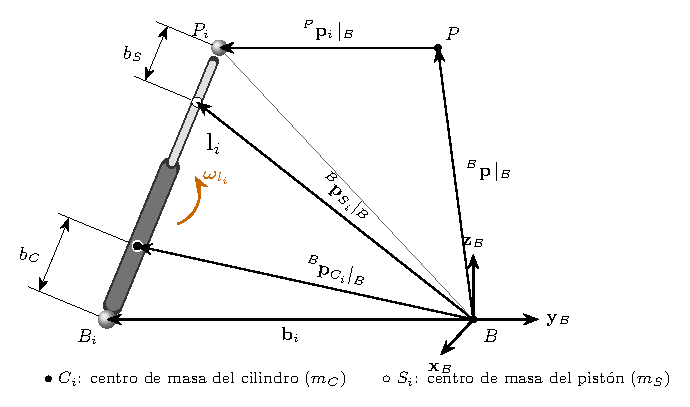
\includegraphics[width=\linewidth]{cuerpos_pata.pdf}
\end{minipage}\hfill
\begin{minipage}[t]{0.47\textwidth}\vspace{0pt}
Del diagrama, recorriendo los caminos desde el origen de $\{B\}$:

\smallskip
\textbf{Plataforma}
\[
\text{Origen}\xrightarrow{\ \vect p\ }P ;\quad \vect r_P = \vect p
\]
\textbf{Cilindro}
\[
\text{Origen}\xrightarrow{\ \vect b_i\ }B_i\xrightarrow{\ b_C\hat{\vect l}_i\ }C_i ;\quad \vect r_{C_i} = \vect b_i + b_C\hat{\vect l}_i
\]
\textbf{Pistón}
\[
\text{Origen}\xrightarrow{\ \vect p\ }P\xrightarrow{\ \vect R\vect s_i\ }P_i\xrightarrow{\ -b_S\hat{\vect l}_i\ }S_i
\]
\[
\vect r_{S_i} = \vect p + \vect R\vect s_i - b_S\hat{\vect l}_i
\]
Alturas, con $b_{i,z} = 0$:
\[
z_P = z ;\quad z_{C_i} = b_C\hat l_{i,z} ;\quad z_{S_i} = z_{P_i} - b_S\hat l_{i,z}
\]
\end{minipage}

% -----------------------------------------------------------------------------------------------
\subsection{Paso 3: velocidad de cada cuerpo}

Derivamos cada posición del Paso 2 y la escribimos como una matriz por $\vect\nu$
Recordando que:
\begin{gather*}
\dot{\vect l}_i = \vect A_i\vect\nu,\quad \vect A_i = [\vect I_3\ \ \sk{\vect p}_i\T];\qquad
\vect\omega_{l_i} = \vect J_{D_i}\vect\nu,\quad \vect J_{D_i} = \sk{\bar{\vect l}}_i\vect A_i;\qquad
\dot{\hat{\vect l}}_i = \vect\omega_{l_i}\times\hat{\vect l}_i;\qquad
\vect\omega\times\vect a = \sk{\vect a}\T\vect\omega .
\end{gather*}

\paragraph{Plataforma:}
$\displaystyle \dot{\vect r}_P  = \dot{\vect p} = \vect v = \begin{bmatrix}\vect I_3 & \vect 0\end{bmatrix}\begin{bmatrix}\vect v\\ \vect\omega\end{bmatrix} = \begin{bmatrix}\vect I_3 & \vect 0\end{bmatrix}\vect\nu$ ; $\displaystyle \vect\omega_P  = \vect\omega = \begin{bmatrix}\vect 0 & \vect I_3\end{bmatrix}\vect\nu .$

\paragraph{Cilindro $i$:}
$\displaystyle \dot{\vect r}_{C_i}  = \frac{d}{dt}\left(\vect b_i + b_C\hat{\vect l}_i\right) = \vect 0 + b_C\,\dot{\hat{\vect l}}_i \ \text{\small($\vect b_i$, $b_C$ constantes)} = b_C\,\vect\omega_{l_i}\times\hat{\vect l}_i = b_C\,\sk{\hat{\vect l}}_i\T\vect\omega_{l_i} = b_C\,\sk{\hat{\vect l}}_i\T\vect J_{D_i}\vect\nu \equiv \vect J_{B_i}\vect\nu,$ ; $\displaystyle \boxed{\vect J_{B_i} = b_C\,\sk{\hat{\vect l}}_i\T\vect J_{D_i}}\ (3\times6)$ ; $\displaystyle \vect\omega_{C_i}  = \vect\omega_{l_i} = \vect J_{D_i}\vect\nu .$

\paragraph{Pistón $i$:}
$\displaystyle \dot{\vect r}_{S_i}  = \frac{d}{dt}\left(\vect p + \vect R\vect s_i\right) - \frac{d}{dt}\left(b_S\hat{\vect l}_i\right) = \left(\vect v + \vect\omega\times\vect R\vect s_i\right) - b_S\,\vect\omega_{l_i}\times\hat{\vect l}_i = \vect A_i\vect\nu - b_S\sk{\hat{\vect l}}_i\T\vect\omega_{l_i} = \vect A_i\vect\nu - b_S\sk{\hat{\vect l}}_i\T\sk{\bar{\vect l}}_i\vect A_i\vect\nu = \left(\vect I_3 - b_S\sk{\hat{\vect l}}_i\T\sk{\bar{\vect l}}_i\right)\vect A_i\vect\nu \equiv \vect J_{G_i}\vect\nu,$ ; $\displaystyle \boxed{\vect J_{G_i} = \left(\vect I_3 - b_S\sk{\hat{\vect l}}_i\T\sk{\bar{\vect l}}_i\right)\vect A_i}\ (3\times6)$ ; $\displaystyle \vect\omega_{S_i}  = \vect\omega_{l_i} = \vect J_{D_i}\vect\nu .$

\paragraph{Reemplazando $\vect\nu = \vect T\dot{\vect q}$:}
$\displaystyle \dot{\vect r}_P  = [\vect I_3\ \ \vect 0]\vect T\dot{\vect q},   \vect\omega_P  = [\vect 0\ \ \vect I_3]\vect T\dot{\vect q}$ ; $\displaystyle \dot{\vect r}_{C_i}  = \vect J_{B_i}\vect T\dot{\vect q},   \vect\omega_{C_i}  = \vect J_{D_i}\vect T\dot{\vect q}$ ; $\displaystyle \dot{\vect r}_{S_i}  = \vect J_{G_i}\vect T\dot{\vect q},   \vect\omega_{S_i}  = \vect J_{D_i}\vect T\dot{\vect q}.$

% -----------------------------------------------------------------------------------------------
\subsection{Paso 4: energía cinética y matriz de inercia}

Sumamos la energía cinética de los 13 cuerpos

\paragraph{Un cuerpo:}
\begin{equation*}
\mathcal T_c = \underbrace{\tfrac12m_c\,\dot{\vect r}_c\T\dot{\vect r}_c}_{\text{traslación}} + \underbrace{\tfrac12\vect\omega_c\T\vect I_c|_B\,\vect\omega_c}_{\text{rotación}} .
\end{equation*}

\paragraph{Inercia vista desde la base:} el tensor es constante en ejes del cuerpo, entonces lo pasamos a $\{B\}$ con $\vect R_c$
$\displaystyle \vect H|_c  = \vect I_c|_c\,\vect\omega|_c \ \text{\small(en ejes del cuerpo)}$ ; $\displaystyle \vect\omega|_c  = \vect R_c\T\vect\omega,$ ; $\displaystyle \vect H = \vect R_c\vect H|_c \ \text{\small(cambio de ejes)}$ ; $\displaystyle \vect H  = \vect R_c\vect I_c|_c\vect R_c\T\vect\omega \ \Rightarrow\ \boxed{\vect I_c|_B = \vect R_c\vect I_c|_c\vect R_c\T}$
Para una pieza de la pata tomamos el eje 1 a lo largo de $\hat{\vect l}_i$:
$\displaystyle \vect I_c|_c  = \begin{bmatrix}I_\parallel & 0 & 0\\ 0 & I_\perp & 0\\ 0 & 0 & I_\perp\end{bmatrix} = I_\perp\begin{bmatrix}1 & 0 & 0\\ 0 & 1 & 0\\ 0 & 0 & 1\end{bmatrix} + (I_\parallel - I_\perp)\begin{bmatrix}1 & 0 & 0\\ 0 & 0 & 0\\ 0 & 0 & 0\end{bmatrix} = I_\perp\vect I + (I_\parallel - I_\perp)\vect e_1\vect e_1\T$ ; $\displaystyle \vect I_c|_B  = I_\perp\vect R_c\vect I\vect R_c\T + (I_\parallel - I_\perp)(\vect R_c\vect e_1)(\vect R_c\vect e_1)\T = I_\perp\vect I + (I_\parallel - I_\perp)\hat{\vect l}_i\hat{\vect l}_i\T \ \text{\small($\vect R_c\vect R_c\T = \vect I$, $\vect R_c\vect e_1 = \hat{\vect l}_i$)} = I_\parallel\hat{\vect l}_i\hat{\vect l}_i\T + I_\perp\left(\vect I - \hat{\vect l}_i\hat{\vect l}_i\T\right).$
Como $\vect\omega_{l_i}\perp\hat{\vect l}_i$ ($\hat{\vect l}_i\T\vect\omega_{l_i} = 0$):
\begin{equation*}
\vect I_c|_B\,\vect\omega_{l_i} = I_\parallel\hat{\vect l}_i(\underbrace{\hat{\vect l}_i\T\vect\omega_{l_i}}_{0}) + I_\perp\vect\omega_{l_i} - I_\perp\hat{\vect l}_i(\underbrace{\hat{\vect l}_i\T\vect\omega_{l_i}}_{0}) = I_\perp\vect\omega_{l_i}.
\end{equation*}
Para la plataforma:
\begin{equation*}
\vect I_B = \vect R\,\mathrm{diag}(0.01125,\ 0.01125,\ 0.0225)\,\vect R\T .
\end{equation*}

\paragraph{Reemplazando las velocidades del Paso 3:} con $(\vect X\dot{\vect q})\T = \dot{\vect q}\T\vect X\T$
$\displaystyle \mathcal T_P  = \tfrac12m_P\,\dot{\vect q}\T\vect T\T[\vect I_3\ \vect 0]\T[\vect I_3\ \vect 0]\vect T\dot{\vect q} + \tfrac12\dot{\vect q}\T\vect T\T[\vect 0\ \vect I_3]\T\vect I_B[\vect 0\ \vect I_3]\vect T\dot{\vect q} = \tfrac12\dot{\vect q}\T\vect T\T\underbrace{\begin{bmatrix}m_P\vect I_3 & \vect 0\\ \vect 0 & \vect I_B\end{bmatrix}}_{\vect I_P|_B}\vect T\dot{\vect q}$ ; $\displaystyle \mathcal T_{C_i}  = \tfrac12m_C(\vect J_{B_i}\vect T\dot{\vect q})\T(\vect J_{B_i}\vect T\dot{\vect q}) + \tfrac12I_{C,\perp}(\vect J_{D_i}\vect T\dot{\vect q})\T(\vect J_{D_i}\vect T\dot{\vect q}) = \tfrac12\dot{\vect q}\T\vect T\T\left(m_C\vect J_{B_i}\T\vect J_{B_i} + I_{C,\perp}\vect J_{D_i}\T\vect J_{D_i}\right)\vect T\dot{\vect q}$ ; $\displaystyle \mathcal T_{S_i}  = \tfrac12\dot{\vect q}\T\vect T\T\left(m_S\vect J_{G_i}\T\vect J_{G_i} + I_{S,\perp}\vect J_{D_i}\T\vect J_{D_i}\right)\vect T\dot{\vect q}.$
En la primera línea: $[\vect I_3\ \vect 0]\T[\vect I_3\ \vect 0] = \begin{bmatrix}\vect I_3\\ \vect 0\end{bmatrix}[\vect I_3\ \vect 0] = \begin{bmatrix}\vect I_3 & \vect 0\\ \vect 0 & \vect 0\end{bmatrix}$ y $[\vect 0\ \vect I_3]\T\vect I_B[\vect 0\ \vect I_3] = \begin{bmatrix}\vect 0 & \vect 0\\ \vect 0 & \vect I_B\end{bmatrix}$; sumadas dan $\vect I_P|_B$.

\paragraph{Suma de los 13 cuerpos:}
$\displaystyle \mathcal T  = \mathcal T_P + \sum_{i=1}^6\mathcal T_{C_i} + \sum_{i=1}^6\mathcal T_{S_i} = \tfrac12\dot{\vect q}\T\,\vect T\T\Bigl[\vect I_P|_B + \sum_{i=1}^6\bigl(m_C\vect J_{B_i}\T\vect J_{B_i} + m_S\vect J_{G_i}\T\vect J_{G_i} + (I_{C,\perp} + I_{S,\perp})\vect J_{D_i}\T\vect J_{D_i}\bigr)\Bigr]\vect T\,\dot{\vect q} \equiv \tfrac12\dot{\vect q}\T\vect M(\vect q)\dot{\vect q},$
\begin{equation}
\boxed{\vect M(\vect q) = \vect T\T\left[\vect I_P|_B + \sum_{i=1}^6\left(m_C\vect J_{B_i}\T\vect J_{B_i} + m_S\vect J_{G_i}\T\vect J_{G_i} + (I_{C,\perp} + I_{S,\perp})\vect J_{D_i}\T\vect J_{D_i}\right)\right]\vect T}\quad(6\times6).
\label{eq:M}
\end{equation}

\paragraph{Propiedades:}
$\displaystyle \vect M\T  = \vect T\T\left[\cdots\right]\T\vect T = \vect M \ \text{\small(cada sumando es $\vect X\T\vect Y\vect X$ con $\vect Y = \vect Y\T$)}$ ; $\displaystyle \dot{\vect q}\T\vect M\dot{\vect q}  = 2\mathcal T \ge m_P\lVert\vect v\rVert^2 + \vect\omega\T\vect I_B\vect\omega > 0\allowbreak\quad(\dot{\vect q}\ne\vect 0) \ \text{\small($\vect M \succ 0$)}$

% -----------------------------------------------------------------------------------------------
\subsection{Paso 5: energía potencial}

La energía potencial es el peso de cada cuerpo por su altura del Paso 2:
$\displaystyle \mathcal V  = m_Pg\,z_P + \sum_{i=1}^6m_Cg\,z_{C_i} + \sum_{i=1}^6m_Sg\,z_{S_i} = g\left(m_Pz + \sum_{i=1}^6m_Cb_C\hat l_{i,z} + \sum_{i=1}^6m_S\left(z_{P_i} - b_S\hat l_{i,z}\right)\right),$ ; $\displaystyle g = 9.80665\ \text{m/s}^2 .$

% -----------------------------------------------------------------------------------------------
\subsection{Paso 6: trabajo de los actuadores y de la perturbación}

Las fuerzas de los actuadores no salen de un potencial, entonces las consideramos por trabajo virtual:
$\displaystyle \delta W_{act}  = \sum_{i=1}^6F_i\,\delta l_i = \vect F\T\delta\vect l = \vect F\T\vect J\vect T\,\delta\vect q \ \text{\small($\delta\vect l = \vect J\vect T\delta\vect q$)} = \left[(\vect J\vect T)\T\vect F\right]\T\delta\vect q \ \text{\small($\vect a\T\vect X\vect b = (\vect X\T\vect a)\T\vect b$)}$ ; $\displaystyle \delta W  = \delta W_{act} + \boldsymbol\tau_d\T\delta\vect q = \vect Q\T\delta\vect q,$
\begin{equation}
\boxed{\vect Q = (\vect J\vect T)\T\vect F + \boldsymbol\tau_d},\qquad |F_i| \le \Fmax\ \text{N}.
\label{eq:Qact}
\end{equation}

% -----------------------------------------------------------------------------------------------
\subsection{Paso 7: ecuación de Euler--Lagrange}

Con la energía cinética y la potencial armamos el lagrangiano $L(\vect q, \dot{\vect q}) = \mathcal T - \mathcal V = \tfrac12\dot{\vect q}\T\vect M(\vect q)\dot{\vect q} - \mathcal V(\vect q)$ y aplicamos la ecuación de Euler--Lagrange con las fuerzas generalizadas del Paso 6, $\dfrac{d}{dt}\dfrac{\partial L}{\partial\dot{\vect q}} - \dfrac{\partial L}{\partial\vect q} = \vect Q$, donde $\dfrac{\partial L}{\partial\dot q_i} = \sum_kM_{ik}\dot q_k$ ; $\dfrac{d}{dt}\dfrac{\partial L}{\partial\dot q_i} = \sum_kM_{ik}\ddot q_k + \sum_{j,k}\dfrac{\partial M_{ik}}{\partial q_j}\dot q_j\dot q_k$ ; $\dfrac{\partial L}{\partial q_i} = \tfrac12\sum_{j,k}\dfrac{\partial M_{jk}}{\partial q_i}\dot q_j\dot q_k - \dfrac{\partial\mathcal V}{\partial q_i}$ ; reemplazando y agrupando lo que multiplica a $\dot q_k$:
\begin{equation}
\boxed{\vect M(\vect q)\,\ddot{\vect q} + \vect C(\vect q, \dot{\vect q})\,\dot{\vect q} + \vect g(\vect q) = (\vect J\vect T)\T\vect F + \boldsymbol\tau_d}
\label{eq:movimiento}
\end{equation}
donde $M_{ik}$ es la ec.~\eqref{eq:M} ; $C_{ik} = \sum_j\left(\dfrac{\partial M_{ik}}{\partial q_j} - \tfrac12\dfrac{\partial M_{jk}}{\partial q_i}\right)\dot q_j$ ; $g_i = \dfrac{\partial\mathcal V}{\partial q_i}$

\begin{figure}[h]
\centering
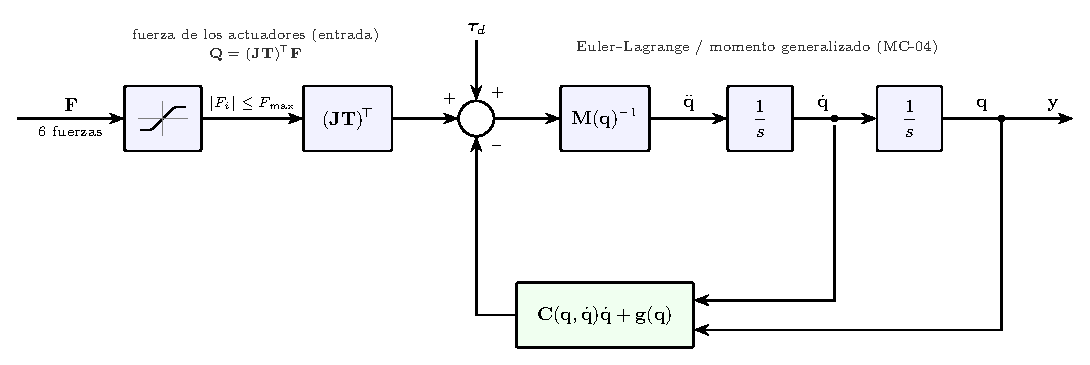
\includegraphics[width=0.92\textwidth]{diagrama_bloques_planta.pdf}
\caption{Diagrama de bloques de la EDO~\eqref{eq:movimiento}.}
\label{fig:bloques}
\end{figure}

% -----------------------------------------------------------------------------------------------
\subsection{Paso 8: el vector $\vect g(\vect q)$}

Para $g_i = \partial\mathcal V/\partial q_i$ usamos los Jacobianos de traslación del Paso 3, $\vect J_c^{lin} = [\vect I_3\ \vect 0]$ (plataforma), $\vect J_{B_i}$ (cilindro), $\vect J_{G_i}$ (pistón): $\mathcal V = \sum_cm_cg\,\hat{\vect z}\T\vect r_c$ ; como $\dot{\vect r}_c = \dfrac{\partial\vect r_c}{\partial\vect q}\dot{\vect q} = \vect J_c^{lin}\vect T\dot{\vect q}$ entonces $\dfrac{\partial\vect r_c}{\partial\vect q} = \vect J_c^{lin}\vect T$ ; $\dfrac{\partial\mathcal V}{\partial\vect q} = \sum_cm_cg\left(\hat{\vect z}\T\vect J_c^{lin}\vect T\right)\T = \vect T\T\sum_c(\vect J_c^{lin})\T m_cg\,\hat{\vect z}$
\begin{equation}
\boxed{\vect g(\vect q) = \vect T\T\left(\begin{bmatrix}m_Pg\,\hat{\vect z}\\ \vect 0\end{bmatrix} + \sum_{i=1}^6\left(\vect J_{B_i}\T m_Cg\,\hat{\vect z} + \vect J_{G_i}\T m_Sg\,\hat{\vect z}\right)\right)}
\label{eq:g}
\end{equation}

% -----------------------------------------------------------------------------------------------
\subsection{Paso 9: EDO de primer orden}

Consideremos como estados la posición y la velocidad:
$\displaystyle \vect x_1  = \vect q,$ ; $\displaystyle \vect x_2 = \dot{\vect q},$ ; $\displaystyle \vect x = \begin{bmatrix}\vect x_1\\ \vect x_2\end{bmatrix}\in\mathbb R^{12},$ ; $\displaystyle \vect u = \vect F\in\mathbb R^6$ ; $\displaystyle \dot{\vect x}_1  = \dot{\vect q} = \vect x_2$ ; $\displaystyle \vect M\dot{\vect x}_2  = (\vect J\vect T)\T\vect u + \boldsymbol\tau_d - \vect C\vect x_2 - \vect g \ \text{\small(de~\eqref{eq:movimiento})}$ ; $\displaystyle \dot{\vect x}_2  = \vect M^{-1}(\vect x_1)\left[(\vect J\vect T)\T\vect u + \boldsymbol\tau_d - \vect C(\vect x_1, \vect x_2)\vect x_2 - \vect g(\vect x_1)\right] \ \text{\small($\vect M \succ 0 \Rightarrow \exists\,\vect M^{-1}$)}$
\begin{equation*}
\boxed{\dot{\vect x} = \begin{bmatrix}\vect x_2\\ \vect M^{-1}(\vect x_1)\left[(\vect J\vect T)\T\vect u + \boldsymbol\tau_d - \vect C\vect x_2 - \vect g\right]\end{bmatrix},\qquad \vect y = \vect x_1 = \vect q .}
\end{equation*}

% -----------------------------------------------------------------------------------------------
\subsection{Paso 10: números en la configuración nominal}



\paragraph{10.1 Configuración nominal:}
\begin{equation*}
\vect q_0 = (0,\ 0,\ 0.270,\ 0,\ 0,\ 0),\quad \vect R = \vect I,\quad \vect E = \vect I,\quad \vect T = \vect I_6,\quad \vect I_B = \mathrm{diag}(0.01125,\ 0.01125,\ 0.0225).
\end{equation*}

\paragraph{10.2 $\vect J_{B_1}$ y $\vect J_{G_1}$:} $\vect J_{B_1} = b_C\sk{\hat{\vect l}}_1\T\vect J_{D_1}$, $b_C = 0.08$ m
\begin{equation*}
\hat{\vect l}_1 = (-0.2670,\ -0.1563,\ 0.9509),\qquad
\sk{\hat{\vect l}}_1\T = \begin{bmatrix}0 & 0.9509 & 0.1563\\ -0.9509 & 0 & -0.2670\\ -0.1563 & 0.2670 & 0\end{bmatrix},
\end{equation*}
\begin{equation*}
\vect J_{D_1} = \begin{bmatrix}
0 & -3.3491 & -0.5506 & 0.0487 & 0.0487 & -0.2960\\
3.3491 & 0 & 0.9405 & -0.0831 & -0.0831 & 0.2960\\
0.5506 & -0.9405 & 0 & 0 & 0 & -0.0345
\end{bmatrix}
\end{equation*}
\[
\sk{\hat{\vect l}}_1\T\vect J_{D_1} = \begin{bmatrix}
3.2707 & -0.1470 & 0.8943 & -0.0790 & -0.0790 & 0.2761\\
-0.1470 & 3.4358 & 0.5236 & -0.0463 & -0.0463 & 0.2907\\
0.8942 & 0.5235 & 0.3372 & -0.0298 & -0.0298 & 0.1253
\end{bmatrix} ;\quad \vect J_{B_1} = 0.08\,\sk{\hat{\vect l}}_1\T\vect J_{D_1}
\]
Para $\vect J_{G_1}$, $\vect P = \sk{\hat{\vect l}}_1\T\sk{\bar{\vect l}}_1$ son las tres primeras columnas del producto anterior:
{\small\[
\vect I_3 - 0.05\vect P = \begin{bmatrix}1 - 0.1635 & 0.0074 & -0.0447\\ 0.0074 & 1 - 0.1718 & -0.0262\\ -0.0447 & -0.0262 & 1 - 0.0169\end{bmatrix} = \begin{bmatrix}0.8365 & 0.0074 & -0.0447\\ 0.0074 & 0.8282 & -0.0262\\ -0.0447 & -0.0262 & 0.9831\end{bmatrix}
\]}
$\vect J_{G_1} = (\vect I_3 - 0.05\vect P)\,[\vect I_3\ \ \sk{\vect p}_1\T]$ con $\sk{\vect p}_1\T = \begin{bmatrix}0 & 0 & 0.08839\\ 0 & 0 & 0.08839\\ -0.08839 & -0.08839 & 0\end{bmatrix}$ ; así:
\begin{gather}
\vect J_{B_1} = \begin{bmatrix}
0.2617 & -0.0118 & 0.0715 & -0.0063 & -0.0063 & 0.0221\\
-0.0118 & 0.2749 & 0.0419 & -0.0037 & -0.0037 & 0.0233\\
0.0715 & 0.0419 & 0.0270 & -0.0024 & -0.0024 & 0.0100
\end{bmatrix},\\
\vect J_{G_1} = \begin{bmatrix}
0.8365 & 0.0074 & -0.0447 & 0.0040 & 0.0040 & 0.0746\\
0.0074 & 0.8282 & -0.0262 & 0.0023 & 0.0023 & 0.0739\\
-0.0447 & -0.0262 & 0.9831 & -0.0869 & -0.0869 & -0.0063
\end{bmatrix}.
\end{gather}

\paragraph{10.3 Matriz de inercia $\vect M_0$:} con $\vect T = \vect I$ en~\eqref{eq:M} y los Jacobianos de las seis patas,
\begin{equation*}
\vect M_0 = \begin{bmatrix}m_P\vect I_3 & \vect 0\\ \vect 0 & \vect I_B\end{bmatrix} + \sum_{i=1}^6\left(m_C\vect J_{B_i}\T\vect J_{B_i} + m_S\vect J_{G_i}\T\vect J_{G_i} + (I_{C,\perp} + I_{S,\perp})\vect J_{D_i}\T\vect J_{D_i}\right)
\end{equation*}
\begin{equation}
\vect M_0 = \begin{bmatrix}\MzeroMat\end{bmatrix}
\end{equation}

\paragraph{10.4 Vector $\vect g_0$:} con $\vect T = \vect I$ en~\eqref{eq:g}, $(\vect J_{B_i})_{zz} = b_C\dfrac{1 - \hat l_{i,z}^2}{l_0}$ y $(\vect J_{G_i})_{zz} = 1 - b_S\dfrac{1 - \hat l_{i,z}^2}{l_0}$ ; por simetría solo sobrevive la componente $z$:
\begin{equation*}
g_z = m_Pg + 6m_Cg\,b_C\frac{1 - \hat l_{i,z}^2}{l_0} + 6m_Sg\left(1 - b_S\frac{1 - \hat l_{i,z}^2}{l_0}\right) = 27.270\ \text{N} ;\qquad \vect g_0 = (0,\ 0,\ 27.270,\ 0,\ 0,\ 0)\ \text{N}
\end{equation*}

\paragraph{10.5 Equilibrio, $F_0$:} $\dot{\vect q} = \ddot{\vect q} = \vect 0$, $\boldsymbol\tau_d = \vect 0$ en~\eqref{eq:movimiento}:
$\displaystyle \vect M_0\cdot\vect 0 + \vect C\cdot\vect 0 + \vect g_0  = \vect J_0\T\vect F_0$ ; $\displaystyle \vect J_0\T\vect F_0  = \vect g_0 .$
con $\vect F_0 = F_0\vect 1$, por simetría solo sobrevive la componente $z$ de $\vect J_0\T\vect 1$, que es $6\hat l_{i,z} = 6(0.9509) = 5.7054$:
\begin{equation*}
5.7054\,F_0 = 27.270 \ \Rightarrow\ F_0 = \frac{27.270}{5.7054} = \Fzero\ \text{N}.
\end{equation*}

% =====================================================================================================
\section{Espacio de estados, linealización y discretización}

\subsection{Modelo no lineal}

Escribimos la EDO en espacio de estados: $\vect x = [\vect q\T\ \dot{\vect q}\T]\T\in\mathbb R^{12}$, $\vect u = \vect F\in\mathbb R^6$, $\vect y = \vect q$; de~\eqref{eq:movimiento} con $\vect M$ invertible:
\begin{equation}
\dot{\vect x} = \vect f(\vect x, \vect u) = \begin{bmatrix}\dot{\vect q}\\ \vect M^{-1}(\vect q)\,\vect h(\vect q, \dot{\vect q}, \vect u)\end{bmatrix},\qquad
\vect h = (\vect J\vect T)\T\vect u + \boldsymbol\tau_d - \vect C\dot{\vect q} - \vect g .
\label{eq:fnl}
\end{equation}

\subsection{Linealización}

Para diseñar los controladores necesitamos un modelo lineal; para ello aplicamos Taylor de primer orden en el reposo.

\paragraph{Paso 1: punto de equilibrio:} $\vect x_0 = [0\ 0\ h_0\ 0\ 0\ 0\ \ \vect 0]\T$, $\vect u_0 = \vect F_0 = F_0\vect 1$, con $\vect h(\vect q_0, \vect 0, \vect u_0) = \vect 0$.

\paragraph{Paso 2: serie de Taylor:} $\delta\vect x = \vect x - \vect x_0$, $\delta\vect u = \vect u - \vect u_0$
$\displaystyle \dot{\vect x} = \vect f(\vect x_0 + \delta\vect x,\ \vect u_0 + \delta\vect u)  = \vect f(\vect x_0, \vect u_0) + \frac{\partial\vect f}{\partial\vect x}\Big|_0\delta\vect x + \frac{\partial\vect f}{\partial\vect u}\Big|_0\delta\vect u + \text{(términos de orden 2)} \approx \vect 0 + \vect A\,\delta\vect x + \vect B\,\delta\vect u \ \text{\small(en el equilibrio $\vect f(\vect x_0, \vect u_0) = \vect 0$)}$
\begin{gather*}
\vect x_0 = \text{cte} \Rightarrow \dot{\vect x} = \delta\dot{\vect x};\qquad \delta\dot{\vect x} \approx \vect A\,\delta\vect x + \vect B\,\delta\vect u,\quad \vect A = \frac{\partial\vect f}{\partial\vect x}\Big|_0\ (12\times12),\quad \vect B = \frac{\partial\vect f}{\partial\vect u}\Big|_0\ (12\times6), \\
\vect f_{1:6} = \dot{\vect q}:\quad \frac{\partial\dot{\vect q}}{\partial\vect q} = \vect 0,\quad \frac{\partial\dot{\vect q}}{\partial\dot{\vect q}} = \vect I_6,\quad \frac{\partial\dot{\vect q}}{\partial\vect u} = \vect 0;\qquad \vect f_{7:12} = \vect M^{-1}\vect h .
\end{gather*}

\paragraph{Paso 3: derivada de $\vect M^{-1}\vect h$:} Para cualquier variable $\xi$ (una componente de $\vect q$, de $\dot{\vect q}$ o de $\vect u$):
$\displaystyle \frac{\partial}{\partial\xi}\left(\vect M^{-1}\vect h\right)  = \frac{\partial\vect M^{-1}}{\partial\xi}\,\vect h + \vect M^{-1}\frac{\partial\vect h}{\partial\xi} \ \text{\small(regla del producto)} = \frac{\partial\vect M^{-1}}{\partial\xi}\,\underbrace{\vect h_0}_{=\,\vect 0} + \vect M_0^{-1}\frac{\partial\vect h}{\partial\xi}\Big|_0 \ \text{\small(evaluando en el equilibrio)}$
$\vect h_0 = \vect 0$ (reposo) $\Rightarrow$ no hace falta derivar $\vect M^{-1}$.

\paragraph{Paso 4: términos de velocidad:} Coriolis es cuadrático en la velocidad
\begin{equation*}
\vect C(\vect q, \dot{\vect q})\dot{\vect q} = \mathcal O(\lVert\dot{\vect q}\rVert^2) \Rightarrow \frac{\partial(\vect C\dot{\vect q})}{\partial\dot{\vect q}}\Big|_{\dot{\vect q} = \vect 0} = \vect 0;\qquad \text{sin disipación} \Rightarrow \frac{\partial\vect h}{\partial\dot{\vect q}}\Big|_0 = \vect 0 .
\end{equation*}

\paragraph{Paso 5: términos de posición y de entrada:} De $\vect h = (\vect J\vect T)\T\vect u + \boldsymbol\tau_d - \vect C\dot{\vect q} - \vect g$:
$\displaystyle \frac{\partial\vect h}{\partial\vect u}\Big|_0  = (\vect J\vect T)\T\Big|_{\vect q_0} = \vect J_0\T \ \text{\small($\vect h$ es lineal en $\vect u$; $\vect T_0 = \vect I$)}$ ; $\displaystyle \frac{\partial\vect h}{\partial\vect q}\Big|_0  = \frac{\partial}{\partial\vect q}\left[(\vect J\vect T)\T\vect u_0 - \vect g\right]_{\vect q_0} \equiv -\vect K_q \ \text{\small(evaluando $\vect u = \vect u_0$, $\dot{\vect q} = \vect 0$)}$
Con el signo menos la fuerza neta queda $-\vect K_q\delta\vect q$, como en un resorte.

\paragraph{Ensamble de $\vect A$ y $\vect B$:} Filas 1--6: $\delta\dot{\vect q}$; filas 7--12: $\delta\ddot{\vect q}$; columnas 1--6: $\delta\vect q$; columnas 7--12: $\delta\dot{\vect q}$.
$\displaystyle \text{filas 1--6:} \allowbreak\quad \frac{d}{dt}\delta\vect q = \underbrace{\vect 0}_{\partial\dot{\vect q}/\partial\vect q}\delta\vect q + \underbrace{\vect I_6}_{\partial\dot{\vect q}/\partial\dot{\vect q}}\delta\dot{\vect q} + \underbrace{\vect 0}_{\partial\dot{\vect q}/\partial\vect u}\delta\vect u$ ; $\displaystyle \text{filas 7--12:} \allowbreak\quad \frac{d}{dt}\delta\dot{\vect q} = \underbrace{\vect M_0^{-1}(-\vect K_q)}_{\text{Pasos 3 y 5}}\delta\vect q + \underbrace{\vect 0}_{\text{Paso 4}}\delta\dot{\vect q} + \underbrace{\vect M_0^{-1}\vect J_0\T}_{\text{Pasos 3 y 5}}\delta\vect u .$
$\delta\vect y = \delta\vect q = \vect I_6\delta\vect q + \vect 0\,\delta\dot{\vect q}$ $\Rightarrow$ $\vect C_y = [\vect I_6\ \ \vect 0]$ ($6\times12$):
\begin{equation}
\vect A = \begin{bmatrix}\vect 0 & \vect I_6\\ \vect A_{21} & \vect 0\end{bmatrix},\qquad
\vect B = \begin{bmatrix}\vect 0\\ \vect B_2\end{bmatrix},\qquad
\vect A_{21} = -\vect M_0^{-1}\vect K_q,\qquad
\vect B_2 = \vect M_0^{-1}\vect J_0\T,\qquad \vect C_y = [\vect I_6\ \ \vect 0].
\label{eq:AB}
\end{equation}
\paragraph{Paso 6: $\vect K_q$ como hessiana:}
\begin{gather*}
\dot l_i = \frac{\partial l_i}{\partial\vect q}\dot{\vect q} = \vect J_i\vect T\dot{\vect q}\ \ \forall\dot{\vect q} \ \Rightarrow\ \frac{\partial l_i}{\partial\vect q} = \vect J_i\vect T, \\
(\vect J\vect T)\T\vect F_0 = \sum_iF_0\left(\frac{\partial l_i}{\partial\vect q}\right)\T = F_0\sum_i\nabla_{\vect q}l_i,\qquad \vect g = \nabla_{\vect q}\mathcal V_g,
\end{gather*}
\begin{equation}
\vect K_q = \nabla^2_{\vect q}\Big(\mathcal V_g - F_0\sum_{i=1}^6 l_i\Big)\Big|_{\vect q_0}
= \underbrace{-F_0\sum_{i=1}^6\nabla^2_{\vect q}l_i}_{\text{precarga}} + \underbrace{\nabla^2_{\vect q}\mathcal V_g}_{\text{peso de las patas}},
\label{eq:Kq}
\end{equation}
simétrica (hessiana); $m_Pgz$ es lineal en $\vect q$ $\Rightarrow$ no aporta:
\begin{center}
\begin{tabular}{|l|r|r|r|}
\hline
Entrada de $\vect K_q$ & Precarga & Peso de las patas & Total \\ \hline
$xx$, $yy$ [N/m] & $-96.162$ & $-17.831$ & $-113.99$ \\ \hline
$zz$ [N/m] & $-9.670$ & $-5.981$ & $-15.651$ \\ \hline
$\phi\phi$, $\theta\theta$ [N\,m/rad] & $-0.2158$ & $-0.0756$ & $-0.2915$ \\ \hline
$\psi\psi$ [N\,m/rad] & $-1.7172$ & $-0.2957$ & $-2.0129$ \\ \hline
\end{tabular}
\end{center}
más el acoplamiento $K_{q,x\theta} = -K_{q,y\phi} = 0.6533$ N/rad; las demás entradas son nulas por la simetría ternaria de la plataforma.

Diagonal $< 0$: precarga y peso de las patas desestabilizan.

Evaluando en el equilibrio:
\begin{gather}
\vect A_{21} = \begin{bmatrix}\AtwoOneMat\end{bmatrix}\ \text{s}^{-2},\\
\vect B_2 = \begin{bmatrix}\BtwoMat\end{bmatrix}.
\end{gather}

\subsection{Rigidez geométrica negativa e inestabilidad en lazo abierto}

Veamos por qué la planta es inestable.

\paragraph{Origen físico:} fuerza constante $F_0$ en la pata $\Rightarrow$ $\mathcal V_F = -F_0\,l_i(\vect q)$. Con $l = \lVert\vect r - \vect b_i\rVert$:
$\displaystyle \nabla_{\vect r}l  = \frac{\partial}{\partial\vect r}\sqrt{(\vect r - \vect b_i)\T(\vect r - \vect b_i)} = \frac{2(\vect r - \vect b_i)}{2\sqrt{(\vect r - \vect b_i)\T(\vect r - \vect b_i)}} = \frac{\vect r - \vect b_i}{l} = \hat{\vect l}_i \ \text{\small(cadena)}$ ; $\displaystyle \nabla^2_{\vect r}l  = \frac{\partial}{\partial\vect r}\left(\frac{\vect r - \vect b_i}{l}\right) = \frac{\vect I_3}{l} - \frac{(\vect r - \vect b_i)}{l^2}\,(\nabla_{\vect r}l)\T \ \text{\small(cociente)} = \frac{\vect I_3}{l} - \frac{\vect l_i\hat{\vect l}_i\T}{l^2} = \frac{1}{l}\left(\vect I_3 - \hat{\vect l}_i\hat{\vect l}_i\T\right) \ \text{\small($\vect l_i = l\,\hat{\vect l}_i$)}$
Miro el signo de esa matriz y sus valores propios:
\begin{gather*}
\vect w\T(\vect I - \hat{\vect l}\hat{\vect l}\T)\vect w = \lVert\vect w\rVert^2 - (\hat{\vect l}\T\vect w)^2 \ge 0\quad(\text{Cauchy--Schwarz},\ \lVert\hat{\vect l}\rVert = 1),\\
\lambda\left(\tfrac1l(\vect I - \hat{\vect l}\hat{\vect l}\T)\right) = \{0\ (\parallel\hat{\vect l}),\ \tfrac1l,\ \tfrac1l\ (\perp\hat{\vect l})\}.
\end{gather*}

Por lo tanto la rigidez es negativa en las dos direcciones perpendiculares a la pata:
\begin{equation*}
\nabla^2\mathcal V_F = -F_0\nabla^2l = -\frac{F_0}{l}\left(\vect I_3 - \hat{\vect l}_i\hat{\vect l}_i\T\right),\qquad \frac{F_0}{l_0} = \frac{4.779}{0.28393} = 16.83\ \text{N/m}\ \text{(negativa, }\perp\text{ a la pata)}.
\end{equation*}

\paragraph{Espectro:} $\vect A = \begin{bmatrix}\vect 0 & \vect I\\ \vect A_{21} & \vect 0\end{bmatrix}$, escribimos $\vect A\vect w = \lambda\vect w$ por bloques con $\vect w = [\vect w_1;\ \vect w_2]$:
$\displaystyle \text{fila de arriba:} \allowbreak\quad \vect 0\cdot\vect w_1 + \vect I\vect w_2 = \lambda\vect w_1 \ \Rightarrow\ \vect w_2 = \lambda\vect w_1$ ; $\displaystyle \text{fila de abajo:} \allowbreak\quad \vect A_{21}\vect w_1 + \vect 0\cdot\vect w_2 = \lambda\vect w_2 = \lambda(\lambda\vect w_1) = \lambda^2\vect w_1 ,$
$\lambda^2\in\lambda(\vect A_{21})$, $\vect w_1 \ne \vect 0$ $\Rightarrow$ $\lambda = \pm\sqrt\mu$, $\mu\in\{\EigAtwoOne\}$ s$^{-2}$, todos $> 0$:
\begin{equation}
\lambda(\vect A) = \{\PolosLA\}\ \text{s}^{-1}:
\end{equation}
6 polos reales $> 0$ $\Rightarrow$ \textbf{inestable en lazo abierto}; perturbación $\sim e^{\SigmaMax t}$.
\begin{ojo}
Calculamos el tiempo en que se duplica una perturbación y lo comparamos con $T_s$:
\begin{gather*}
\sigma = 7.62\ \text{s}^{-1},\qquad e^{\sigma t} = 2 \ \Rightarrow\ t = \frac{\ln2}{\sigma} = 0.091\ \text{s}, \\
T_s = 2\ \text{ms} \ll 0.091\ \text{s}.
\end{gather*}
\end{ojo}

\subsection{Modelo en las coordenadas de las patas}

Como el PID actúa pata por pata, escribimos el modelo en longitudes de pata.

Hacemos entonces el cambio de variable a longitudes:
$\displaystyle \delta\vect l  = \vect J_0\delta\vect q \ \Rightarrow\ \delta\vect q = \vect J_0^{-1}\delta\vect l,\allowbreak\quad \delta\ddot{\vect q} = \vect J_0^{-1}\delta\ddot{\vect l} \ \text{\small($\vect J_0$ constante; $\vect T_0 = \vect I$)}$ ; $\displaystyle \vect M_0\delta\ddot{\vect q}  = \vect J_0\T\delta\vect F - \vect K_q\delta\vect q \ \text{\small(modelo lineal: $\vect M_0\times$ la fila de abajo de $\vect A$, $\vect B$)}$ ; $\displaystyle \vect M_0\vect J_0^{-1}\delta\ddot{\vect l}  = \vect J_0\T\delta\vect F - \vect K_q\vect J_0^{-1}\delta\vect l \ \text{\small(reemplazando $\delta\vect q$)}$ ; $\displaystyle \vect J_0^{-\top}\vect M_0\vect J_0^{-1}\delta\ddot{\vect l}  = \delta\vect F - \vect J_0^{-\top}\vect K_q\vect J_0^{-1}\delta\vect l \ \text{\small(multiplicando por $\vect J_0^{-\top}$; $\vect J_0^{-\top}\vect J_0\T = \vect I$)}$
y como $\vect M_0\vect A_{21} = -\vect K_q$, el último término es $+\vect J_0^{-\top}(\vect M_0\vect A_{21})\vect J_0^{-1}\delta\vect l$:
\begin{equation}
\underbrace{\vect J_0^{-\top}\vect M_0\vect J_0^{-1}}_{\boldsymbol\Lambda}\,\delta\ddot{\vect l} = \delta\vect F + \underbrace{\vect J_0^{-\top}\left(\vect M_0\vect A_{21}\right)\vect J_0^{-1}}_{\vect K_l}\,\delta\vect l .
\label{eq:patas}
\end{equation}
\begin{gather*}
\lambda(\boldsymbol\Lambda) = \{\LamEigs\}\ \text{kg}, \\ \lambda(\vect K_l) = \{\KlEigs\}\ \text{N/m}, \\
\delta\vect F = -K_p\delta\vect l \ \Rightarrow\ \text{rigidez neta } K_p\vect I - \vect K_l \succ 0 \ \Leftrightarrow\ \boxed{K_p > \lambda_{\max}(\vect K_l) = \KlMax\ \text{N/m}} .
\end{gather*}

Tomamos el término diagonal de~\eqref{eq:patas} para la pata 1: $m = \Lambda_{11} = \mLeg$ kg, $k = K_{l,11} = \kLeg$ N/m; masa con las demás libres $1/(\boldsymbol\Lambda^{-1})_{11} = \mEff$ kg.

\subsection{Discretización}

Como el controlador corre cada $T_s = \Ts$ ms, discretizamos con retenedor de orden cero:
\[
\vect x_{k+1} = e^{\vect AT_s}\vect x_k + \left(\int_0^{T_s}e^{\vect A\eta}d\eta\right)\vect B\vect u_k .
\]
Ambos bloques se obtienen con una sola exponencial (Van Loan), porque
\begin{equation*}
\begin{bmatrix}\vect A & \vect B\\ \vect 0 & \vect 0\end{bmatrix}^k = \begin{bmatrix}\vect A^k & \vect A^{k-1}\vect B\\ \vect 0 & \vect 0\end{bmatrix}\quad(k \ge 1):
\end{equation*}
\begin{equation}
\exp\left(\begin{bmatrix}\vect A & \vect B\\ \vect 0 & \vect 0\end{bmatrix}T_s\right) = \begin{bmatrix}\vect A_d & \vect B_d\\ \vect 0 & \vect I\end{bmatrix},\qquad \vect A_d = e^{\vect AT_s},\quad \vect B_d = \int_0^{T_s}e^{\vect A\eta}d\eta\,\vect B .
\end{equation}
\emph{Potencia por bloques.} Por inducción y sumando la serie:
\begin{gather*}
\begin{bmatrix}\vect A^k & \vect A^{k-1}\vect B\\ \vect 0 & \vect 0\end{bmatrix}\begin{bmatrix}\vect A & \vect B\\ \vect 0 & \vect 0\end{bmatrix} = \begin{bmatrix}\vect A^{k+1} & \vect A^k\vect B\\ \vect 0 & \vect 0\end{bmatrix}, \\
\sum_{k\ge1}\frac{T_s^k}{k!}\vect A^{k-1}\vect B = \int_0^{T_s}\sum_{k\ge0}\frac{\vect A^k\eta^k}{k!}d\eta\,\vect B\qquad\left(\int_0^{T_s}\eta^kd\eta = \frac{T_s^{k+1}}{k+1}\right).
\end{gather*}

\paragraph{Forma cerrada:} potencias de $\vect A$
\begin{equation*}
\vect A^2 = \begin{bmatrix}\vect 0 & \vect I\\ \vect A_{21} & \vect 0\end{bmatrix}\begin{bmatrix}\vect 0 & \vect I\\ \vect A_{21} & \vect 0\end{bmatrix} = \begin{bmatrix}\vect 0\cdot\vect 0 + \vect I\vect A_{21} & \vect 0\cdot\vect I + \vect I\cdot\vect 0\\ \vect A_{21}\cdot\vect 0 + \vect 0\cdot\vect A_{21} & \vect A_{21}\vect I + \vect 0\end{bmatrix} = \begin{bmatrix}\vect A_{21} & \vect 0\\ \vect 0 & \vect A_{21}\end{bmatrix},
\end{equation*}
\begin{gather*}
\vect A^{2k} = \mathrm{diag}(\vect A_{21}^k, \vect A_{21}^k),\qquad \vect A^{2k+1} = \vect A^{2k}\vect A = \begin{bmatrix}\vect 0 & \vect A_{21}^k\\ \vect A_{21}^{k+1} & \vect 0\end{bmatrix}, \\
e^{\vect AT_s} = \sum_n\frac{\vect A^nT_s^n}{n!} = \underbrace{\sum_k\frac{\vect A^{2k}T_s^{2k}}{(2k)!}}_{\text{diagonal}} + \underbrace{\sum_k\frac{\vect A^{2k+1}T_s^{2k+1}}{(2k+1)!}}_{\text{fuera de la diagonal}}:
\end{gather*}
\begin{equation}
\vect A_d = \begin{bmatrix}\cosh(\vect ST_s) & \vect S^{-1}\sinh(\vect ST_s)\\ \vect S\sinh(\vect ST_s) & \cosh(\vect ST_s)\end{bmatrix},\qquad
\vect B_d = \begin{bmatrix}\vect A_{21}^{-1}\left(\cosh(\vect ST_s) - \vect I\right)\vect B_2\\ \vect S^{-1}\sinh(\vect ST_s)\,\vect B_2\end{bmatrix},
\label{eq:AdBd}
\end{equation}
Identificando las series y calculando las integrales de $\vect B_d$:
\begin{gather*}
\cosh(\vect ST_s) = \sum_k\frac{\vect A_{21}^kT_s^{2k}}{(2k)!},\qquad \vect S^{-1}\sinh(\vect ST_s) = \sum_k\frac{\vect A_{21}^kT_s^{2k+1}}{(2k+1)!},\qquad \vect S = \vect A_{21}^{1/2}, \\
\frac{d}{d\eta}\sinh(\vect S\eta) = \vect S\cosh(\vect S\eta),\qquad \frac{d}{d\eta}\cosh(\vect S\eta) = \vect S\sinh(\vect S\eta),
\end{gather*}
\begin{gather*}
\int_0^{T_s}\cosh(\vect S\eta)d\eta = \vect S^{-1}\left[\sinh(\vect S\eta)\right]_0^{T_s} = \vect S^{-1}\sinh(\vect ST_s),\\
\int_0^{T_s}\vect S^{-1}\sinh(\vect S\eta)d\eta = \vect S^{-2}\left[\cosh(\vect S\eta)\right]_0^{T_s} = \vect A_{21}^{-1}(\cosh(\vect ST_s) - \vect I),
\end{gather*}
$\vect B = [\vect 0;\ \vect B_2]$ toma solo la segunda columna de bloques. Error frente a Van Loan: $3.7\times10^{-16}$.
\begin{equation*}
\lVert\vect A_{21}\rVert T_s^2 \approx 2\times10^{-4} \Rightarrow \vect A_d \approx \begin{bmatrix}\vect I & T_s\vect I\\ T_s\vect A_{21} & \vect I\end{bmatrix},\qquad \vect B_d \approx \begin{bmatrix}\tfrac12T_s^2\vect B_2\\ T_s\vect B_2\end{bmatrix}.
\end{equation*}

Los polos discretos son $z = e^{\lambda T_s}$:
\begin{gather*}
\vect A\vect w = \lambda\vect w \Rightarrow e^{\vect AT_s}\vect w = \sum_n\frac{(\lambda T_s)^n}{n!}\vect w = e^{\lambda T_s}\vect w, \\
e^{7.62\cdot0.002} = e^{0.01524} = 1.01536 > 1\ \text{(fuera del círculo)},\qquad e^{-0.01524} = 0.98488 .
\end{gather*}
$T_s = 2$ ms (500 Hz): modos rápidos $> 40$ rad/s; con 10 ms el PID no estabilizaba con rigidez lateral suficiente.

\subsection{Propiedades estructurales}

Antes de diseñar revisamos la observabilidad, la controlabilidad y la controlabilidad con integradores:

\begin{itemize}
\item \textbf{Observabilidad.} $\mathcal O = [\vect C_y;\ \vect C_y\vect A;\ \dots]$:
\begin{equation*}
\vect C_y\vect A = \begin{bmatrix}\vect I & \vect 0\end{bmatrix}\begin{bmatrix}\vect 0 & \vect I\\ \vect A_{21} & \vect 0\end{bmatrix} = \begin{bmatrix}\vect I\cdot\vect 0 + \vect 0\cdot\vect A_{21} & \vect I\cdot\vect I + \vect 0\cdot\vect 0\end{bmatrix} = \begin{bmatrix}\vect 0 & \vect I\end{bmatrix},
\end{equation*}
$\begin{bmatrix}\vect C_y\\ \vect C_y\vect A\end{bmatrix} = \begin{bmatrix}\vect I & \vect 0\\ \vect 0 & \vect I\end{bmatrix} = \vect I_{12}$ $\Rightarrow$ rango 12.
\item \textbf{Controlabilidad.} Calculamos las dos primeras potencias:
\begin{equation*}
\vect A\vect B = \begin{bmatrix}\vect 0 & \vect I\\ \vect A_{21} & \vect 0\end{bmatrix}\begin{bmatrix}\vect 0\\ \vect B_2\end{bmatrix} = \begin{bmatrix}\vect B_2\\ \vect 0\end{bmatrix}
\quad\Longrightarrow\quad
[\vect B\ \ \vect A\vect B] = \begin{bmatrix}\vect 0 & \vect B_2\\ \vect B_2 & \vect 0\end{bmatrix}\in\mathbb R^{12\times12}.
\end{equation*}
Intercambio de bloques de columnas: $6\cdot6 = 36$ transposiciones, $(-1)^{36} = +1$:
\begin{equation*}
\det[\vect B\ \ \vect A\vect B] = \det\begin{bmatrix}\vect B_2 & \vect 0\\ \vect 0 & \vect B_2\end{bmatrix} = \det(\vect B_2)^2,
\end{equation*}
\begin{equation*}
\det\vect B_2 = \det(\vect M_0^{-1})\det(\vect J_0\T) = \frac{\det\vect J_0}{\det\vect M_0} = \frac{-2.433\times10^{-3}}{2.091\times10^{-4}} = -11.64 ,
\end{equation*}
$\det[\vect B\ \ \vect A\vect B] = (-11.64)^2 = 135.4 \ne 0$ $\Rightarrow$ rango 12. $\det\vect B_2 \ne 0 \Leftrightarrow \det\vect J_0 \ne 0$: controlable en todo el espacio de trabajo (PBH $\checkmark$).
\item \textbf{Ceros en el origen} (para integradores): rango de $\begin{bmatrix}\vect A & \vect B\\ -\vect C_y & \vect 0\end{bmatrix}\in\mathbb R^{18\times18}$:
\begin{equation*}
\begin{bmatrix}\vect A & \vect B\\ -\vect C_y & \vect 0\end{bmatrix} = \begin{bmatrix}\vect 0 & \vect I & \vect 0\\ \vect A_{21} & \vect 0 & \vect B_2\\ -\vect I & \vect 0 & \vect 0\end{bmatrix}.
\end{equation*}
\begin{equation*}
F_2 \leftarrow F_2 + \vect A_{21}F_3:\ \begin{bmatrix}\vect 0 & \vect I & \vect 0\\ \vect 0 & \vect 0 & \vect B_2\\ -\vect I & \vect 0 & \vect 0\end{bmatrix} \ \Rightarrow\ \text{rango} = 6 + 6 + 6 = 18 .
\end{equation*}
\end{itemize}

% =====================================================================================================
\section{Trayectorias óptimas por cálculo de variaciones}
\label{sec:var}

Ahora buscamos una trayectoria de referencia suave y cercana al destino para que el controlador la siga; para ello consideremos el funcional $\mathcal J[x] = \int_{t_0}^{t_f}F(t, x, \dot x)\,dt$.

\subsection{Primera variación con extremos conocidos o libres}
\label{sec:frontera}

Con $x = x^\star + \epsilon\eta$, la primera variación integrada por partes es
\begin{equation}
\delta\mathcal J = F_{\dot x}\big|_{t_f}\eta(t_f) - F_{\dot x}\big|_{t_0}\eta(t_0) + \int_{t_0}^{t_f}\left(F_x - \frac{d}{dt}F_{\dot x}\right)\eta\,dt = 0
\label{eq:dJfrontera}
\end{equation}
de donde en el interior sale Euler--Lagrange, $F_x - \frac{d}{dt}F_{\dot x} = 0$, y en cada extremo: si es conocido $\eta = 0$ y el término desaparece ; si es libre $\eta$ es arbitrario y $F_{\dot x} = 0$ (condición natural).

\subsection{Casos de frontera A, B, C y D}
\label{sec:casosAD}

Como la EDO es de orden 2 necesitamos una condición por extremo, entonces tenemos 4 combinaciones:

\begin{table}[h]
\centering
\caption{Los cuatro casos de frontera (tiempos $t_0$ y $t_f$ fijos)}
\label{tab:casosfrontera}
\small
\begin{tabular}{|c|l|l|l|}
\hline
Caso & Límite inferior $t_0$ & Límite superior $t_f$ & Condiciones \\ \hline
A & conocido & conocido & $x(t_0) = x_0$, \ $x(t_f) = x_f$ \\ \hline
B & conocido & libre & $x(t_0) = x_0$, \ $F_{\dot x}(t_f) = 0$ \\ \hline
C & libre & conocido & $F_{\dot x}(t_0) = 0$, \ $x(t_f) = x_f$ \\ \hline
D & libre & libre & $F_{\dot x}(t_0) = 0$, \ $F_{\dot x}(t_f) = 0$ \\ \hline
\end{tabular}
\end{table}

Liberar un extremo agranda el conjunto admisible, $\mathcal A_A \subset \mathcal A_B, \mathcal A_C \subset \mathcal A_D$, por lo tanto $\mathcal J^\star_D \le \mathcal J^\star_B,\ \mathcal J^\star_C \le \mathcal J^\star_A$.

\subsection{Casos especiales del integrando}
\label{sec:especiales}

Desarrollando la derivada total, Euler--Lagrange queda
\begin{equation}
F_x - F_{\dot xt} - F_{\dot xx}\,\dot x - F_{\dot x\dot x}\,\ddot x = 0
\label{eq:ELdesarrollada}
\end{equation}
y según de qué variables dependa $F$ se simplifica: si $F = F(t, \dot x)$ (caso I), $F_x = 0$ y $F_{\dot x} = c$ ; si $F = F(t, x, \dot x)$ con $t$ explícito (caso II) hay que resolver~\eqref{eq:ELdesarrollada} completa ; si $F = F(x, \dot x)$ (caso III) vale la identidad de Beltrami
\begin{equation}
\boxed{\dot xF_{\dot x} - F = C}
\label{eq:beltramigeneral}
\end{equation}
y si $F = F(t, x)$ (caso IV) queda la ecuación algebraica $F_x(t, x) = 0$.

\begin{table}[h]
\centering
\caption{Casos especiales del integrando y dónde aparecen en la plataforma}
\label{tab:especiales}
\small
\begin{tabular}{|c|l|l|l|}
\hline
Caso & Integrando & Simplificación & En la plataforma \\ \hline
I & $F(t, \dot x)$ & $F_{\dot x} = c$ & intercepción de una senoidal \\ \hline
II & $F(t, x, \dot x)$, $t$ explícito & ecuación completa & descuento; seguimiento de una onda \\ \hline
III & $F(x, \dot x)$ & $\dot xF_{\dot x} - F = C$ & extremos fijos, final libre, tiempo libre \\ \hline
IV & $F(t, x)$ & $F_x = 0$ & equilibrio estático \\ \hline
\end{tabular}
\end{table}



\subsection{Caso I: estado final sobre una curva (intercepción de una senoidal)}
\label{sec:curva}

Problema: alcanzar con mínimo esfuerzo una referencia que oscila, con el instante de encuentro $T$ libre. Datos: $z_0 = 5$ mm en reposo $\to$ $\phi(t) = A\sin(\omega t)$, $A = 15$ mm, $\omega = 2\pi\cdot0.45 = 2.82743$ rad/s; $F = \tfrac12\dot z^2$; $T$ libre.
\paragraph{Caso I:} $F_z = 0$ (coordenada cíclica) $\Rightarrow F_{\dot z} = \dot z = C_1$: la trayectoria óptima es una recta, $z = z_0 + ct$.
Como $T$ no está fijo usamos la primera variación con extremo móvil,
\begin{equation}
\delta\mathcal J = F_{\dot z}\big|_T\,\delta z_T + \left(F - \dot zF_{\dot z}\right)\big|_T\,\delta T = 0
\label{eq:extremomovil}
\end{equation}
y con el punto final sobre la curva $z = \phi(t)$, $\delta z_T = \dot\phi(T)\,\delta T$, la condición de transversalidad es $\left[F + F_{\dot z}(\dot\phi - \dot z)\right]_T = 0$.
\paragraph{Transversalidad con la curva terminal:} Con $F = \tfrac12\dot z^2$ y $\dot z = c$:
\begin{equation}
\left[F + F_{\dot z}(\dot\phi - \dot z)\right]_{T} = \tfrac12c^2 + c(\dot\phi(T) - c) = c\left(\dot\phi(T) - \tfrac12c\right) = 0\ \Longrightarrow\ c = 2\dot\phi(T).
\end{equation}
\paragraph{Instante de intercepción:} La recta es $z(t) = z_0 + ct$ con $c = 2\dot\phi(T) = 2A\omega\cos(\omega T)$. Sustituyendo en la condición de encuentro $z(T) = \phi(T)$:
\begin{equation*}
G(T) \equiv z_0 + 2A\omega\cos(\omega T)\,T - A\sin(\omega T) = 0,
\end{equation*}
$A\omega = 15\cdot2.82743 = 42.411$ mm/s. Newton, $T_{k+1} = T_k - G(T_k)/G'(T_k)$:
\begin{equation*}
G'(T) = 2A\omega\cos(\omega T) - 2A\omega^2T\sin(\omega T) - A\omega\cos(\omega T) = A\omega\cos(\omega T) - 2A\omega^2T\sin(\omega T).
\end{equation*}
\begin{center}
\begin{tabular}{|c|c|c|c|}
\hline
$k$ & $T_k$ [s] & $G(T_k)$ [mm] & $G'(T_k)$ [mm/s] \\ \hline
0 & 0.50000 & $-3.1807$ & $-111.80$ \\ \hline
1 & 0.47155 & $-0.1677$ & $-99.94$ \\ \hline
2 & 0.46987 & $-0.0006$ & $-99.23$ \\ \hline
3 & 0.46987 & $0.0000$ & $-99.22$ \\ \hline
\end{tabular}
\end{center}
Con $T = 0.46987$ s: $c = 2A\omega\cos(\omega T) = 20.35$ mm/s ; $z(T) = z_0 + cT = A\sin(\omega T) = 14.56$ mm $\checkmark$

\subsection{Maniobra de referencia para los casos II y III}

Consideremos una maniobra de $\vect q_A$ a $\vect q_B$ con el error normalizado:
\begin{equation}
\varepsilon(t) = \frac{q(t) - q_B}{q_A - q_B},\qquad \varepsilon(0) = 1,\qquad q(t) = q_B + \varepsilon(t)\,(q_A - q_B),
\end{equation}
y el funcional de costo
\begin{equation}
\mathcal J[\varepsilon] = \int_0^T\underbrace{\left(\tfrac12\dot\varepsilon^2 + \tfrac12a^2\varepsilon^2\right)}_{F(\varepsilon, \dot\varepsilon)}dt ,
\label{eq:Fvar}
\end{equation}
1.º término: esfuerzo ($\propto\dot l$); 2.º: distancia al destino; $a = 2$ s$^{-1}$, $T = 2$ s, $aT = 4$:
\begin{equation}
F_\varepsilon = a^2\varepsilon,\qquad F_{\dot\varepsilon} = \dot\varepsilon,\qquad \frac{d}{dt}F_{\dot\varepsilon} = \ddot\varepsilon,
\end{equation}
y la ecuación de Euler--Lagrange $F_\varepsilon - \frac{d}{dt}F_{\dot\varepsilon} = 0$ da
\begin{equation}
\boxed{\ddot\varepsilon - a^2\varepsilon = 0}\ \Longrightarrow\ r^2 - a^2 = 0,\ r = \pm a\ \Longrightarrow\ \varepsilon(t) = C_1\cosh(at) + C_2\sinh(at).
\label{eq:ELvar}
\end{equation}
Probando $\varepsilon = e^{rt}$ y pasando a funciones hiperbólicas:
\begin{gather*}
\varepsilon = e^{rt} \Rightarrow (r^2 - a^2)e^{rt} = 0 \Rightarrow r = \pm a \Rightarrow \varepsilon = k_1e^{at} + k_2e^{-at}, \\
\cosh(at) = \tfrac12(e^{at} + e^{-at}),\quad \sinh(at) = \tfrac12(e^{at} - e^{-at}),\quad C_1 = k_1 + k_2,\ C_2 = k_1 - k_2, \\
\tfrac{d}{dt}\cosh(at) = a\sinh(at),\qquad \tfrac{d}{dt}\sinh(at) = a\cosh(at).
\end{gather*}
$F$ sin $t$ $\Rightarrow$ caso III; con descuento $\Rightarrow$ caso II.

\subsection{Caso II: factor de descuento exponencial}
\label{sec:caso2}

Ahora agregamos un factor que pesa más los primeros instantes, $L = e^{-\alpha t}F(\varepsilon, \dot\varepsilon)$; como depende de $t$ es el caso II:
$\displaystyle L_\varepsilon  = e^{-\alpha t}a^2\varepsilon, $ ; $\displaystyle L_{\dot\varepsilon} = e^{-\alpha t}\dot\varepsilon$ ; $\displaystyle \frac{d}{dt}L_{\dot\varepsilon}  = -\alpha e^{-\alpha t}\dot\varepsilon + e^{-\alpha t}\ddot\varepsilon = e^{-\alpha t}(\ddot\varepsilon - \alpha\dot\varepsilon) \ \text{\small(regla del producto)}$ ; $\displaystyle L_\varepsilon - \frac{d}{dt}L_{\dot\varepsilon}  = e^{-\alpha t}\left(a^2\varepsilon - \ddot\varepsilon + \alpha\dot\varepsilon\right) = 0 \ \text{\small(Euler--Lagrange)}$
y dividimos por $e^{-\alpha t} \neq 0$. La ecuación característica de $\ddot\varepsilon - \alpha\dot\varepsilon - a^2\varepsilon = 0$ con $\varepsilon = e^{rt}$ es $r^2 - \alpha r - a^2 = 0$:
\begin{equation}
\boxed{\ddot\varepsilon - \alpha\dot\varepsilon - a^2\varepsilon = 0},\qquad r_{1,2} = \frac{\alpha \pm \sqrt{\alpha^2 + 4a^2}}{2}.
\end{equation}
Con $\alpha = 1$ s$^{-1}$ y $a = 2$ s$^{-1}$: $\alpha^2 + 4a^2 = 17$, $\sqrt{17} = 4.1231$, $r_1 = 2.5616$ y $r_2 = -1.5616$ s$^{-1}$. Con $\varepsilon = C_1e^{r_1t} + C_2e^{r_2t}$ imponemos los extremos:
$\displaystyle \varepsilon(0) = 1: \allowbreak\quad C_1 + C_2 = 1$ ; $\displaystyle \varepsilon(T) = 0: \allowbreak\quad C_1e^{r_1T} + C_2e^{r_2T} = 0 .$
De la segunda, $C_1 = -C_2e^{r_2T}/e^{r_1T}$; reemplazando en la primera, $C_2(1 - e^{r_2T}/e^{r_1T}) = 1$, y multiplicando arriba y abajo por $e^{r_1T}$:
\begin{equation}
C_2 = \frac{e^{r_1T}}{e^{r_1T} - e^{r_2T}},\qquad C_1 = 1 - C_2 = \frac{-e^{r_2T}}{e^{r_1T} - e^{r_2T}} .
\end{equation}
Con $T = 2$ s: $e^{r_1T} = e^{5.1231} = 167.856$, $e^{r_2T} = e^{-3.1231} = 0.04402$, $e^{r_1T} - e^{r_2T} = 167.812$, de modo que $C_2 = 1.00026$ y $C_1 = -2.623\times10^{-4}$.

Evaluando en $t = 1$ s y comprobando Legendre:
$\displaystyle e^{r_1\cdot1}  = 12.9559,$ ; $\displaystyle e^{r_2\cdot1} = 0.20981$ ; $\displaystyle \varepsilon(1)  = 0.206\allowbreak\quad(\text{vs. } 0.133\ \text{sin descuento})$ ; $\displaystyle L_{\dot\varepsilon\dot\varepsilon}  = e^{-\alpha t} > 0\ \text{(Legendre)}.$

\subsection{Caso III (Beltrami): extremos fijos}
\label{sec:caso3}

\eqref{eq:Fvar} no depende de $t$ $\Rightarrow$ Beltrami~\eqref{eq:beltramigeneral}.

\paragraph{Integral primera:} $F_{\dot\varepsilon} = \dot\varepsilon$
\begin{equation}
\dot\varepsilon F_{\dot\varepsilon} - F = \dot\varepsilon^2 - \tfrac12\dot\varepsilon^2 - \tfrac12a^2\varepsilon^2 = \tfrac12\dot\varepsilon^2 - \tfrac12a^2\varepsilon^2 = C .
\label{eq:beltrami}
\end{equation}
\paragraph{Fronteras fijas:} $\varepsilon = D_1\sinh(a(T - t)) + D_2\cosh(a(T - t))$ ($\frac{d^2}{dt^2}$ saca $(-a)^2 = a^2$ $\Rightarrow$ cumple $\ddot\varepsilon = a^2\varepsilon$):
\begin{equation*}
\varepsilon(T) = D_1\sinh0 + D_2\cosh0 = D_2 = 0,\qquad \varepsilon(0) = D_1\sinh(aT) = 1 \Rightarrow D_1 = \frac{1}{\sinh(aT)},
\end{equation*}
\begin{equation}
\boxed{\varepsilon^\star(t) = \frac{\sinh(a(T - t))}{\sinh(aT)}},\qquad
\dot\varepsilon^\star(t) = -\frac{a\cosh(a(T - t))}{\sinh(aT)}.
\label{eq:fijos}
\end{equation}
\paragraph{Comprobación:}
\begin{gather*}
\dot\varepsilon^\star = \frac{-a\cosh(a(T - t))}{\sinh(aT)},\quad \ddot\varepsilon^\star = \frac{a^2\sinh(a(T - t))}{\sinh(aT)} = a^2\varepsilon^\star\ \checkmark, \\
\varepsilon^\star(0) = \frac{\sinh(aT)}{\sinh(aT)} = 1\ \checkmark,\qquad \varepsilon^\star(T) = \frac{\sinh0}{\sinh(aT)} = 0\ \checkmark .
\end{gather*}

\paragraph{Beltrami:} $C$ en $t = T$ y en todo instante
\begin{gather*}
t = T:\ \varepsilon = 0,\ \dot\varepsilon = -\frac{a}{\sinh(aT)} \Rightarrow C = \frac{a^2}{2\sinh^2(aT)}, \\ C = \frac{4}{2\cdot27.2899^2} = \frac{4}{2\cdot744.74} = \frac{4}{1489.48} = 2.69\times10^{-3}, \\
\forall t:\ \tfrac12\dot\varepsilon^2 - \tfrac12a^2\varepsilon^2 = \frac{a^2}{2\sinh^2(aT)}\left[\cosh^2 - \sinh^2\right] = \frac{a^2}{2\sinh^2(aT)}\cdot1 = C\ \checkmark .
\end{gather*}
\paragraph{Valor del funcional:} por partes, $u = \dot\varepsilon$, $dv = \dot\varepsilon\,dt$
$\displaystyle \int_0^T\dot\varepsilon^2dt  = \left[\varepsilon\dot\varepsilon\right]_0^T - \int_0^T\varepsilon\ddot\varepsilon\,dt \ \text{\small(por partes)} = \left[\varepsilon\dot\varepsilon\right]_0^T - a^2\int_0^T\varepsilon^2dt \ \text{\small($\ddot\varepsilon = a^2\varepsilon$)}$
sumando, las integrales de $\varepsilon^2$ se cancelan:
$\displaystyle \mathcal J^\star  = \tfrac12\int_0^T\dot\varepsilon^2dt + \tfrac12a^2\int_0^T\varepsilon^2dt = \tfrac12\left([\varepsilon\dot\varepsilon]_0^T - a^2\int_0^T\varepsilon^2dt\right) + \tfrac12a^2\int_0^T\varepsilon^2dt = \tfrac12[\varepsilon\dot\varepsilon]_0^T = \tfrac12\left(\varepsilon(T)\dot\varepsilon(T) - \varepsilon(0)\dot\varepsilon(0)\right) = \tfrac12\left(0 - 1\cdot\dot\varepsilon(0)\right) \ \text{\small($\varepsilon(T) = 0$, $\varepsilon(0) = 1$)} = -\tfrac12\left(-\frac{a\cosh(aT)}{\sinh(aT)}\right) = \tfrac12a\coth(aT) = \tfrac12\cdot2\cdot\frac{27.3082}{27.2899} = 1.00067 .$
\paragraph{Valores:} Velocidad inicial y punto medio de la maniobra:
\begin{gather*}
\dot\varepsilon^\star(0) = -a\coth(aT) = -2\cdot1.00067 = -2.0013\ \text{s}^{-1},\qquad |\dot q(0)| = 2.0013\cdot15 = 30.0\ \text{mm/s}, \\
\varepsilon^\star(1) = \frac{\sinh(2(2 - 1))}{\sinh(4)} = \frac{\sinh2}{\sinh4} = \frac{3.6269}{27.2899} = 0.133 .
\end{gather*}

\subsection{Caso III: condiciones de segundo orden (Legendre, convexidad y Ritz)}


\paragraph{Legendre:} $F_{\dot\varepsilon\dot\varepsilon} = \frac{\partial^2}{\partial\dot\varepsilon^2}\left(\tfrac12\dot\varepsilon^2\right) = 1 > 0$.
\paragraph{Convexidad (mínimo global):} La Hessiana de $F$ respecto a $(\varepsilon, \dot\varepsilon)$ es
\begin{equation}
\vect H_F = \begin{bmatrix}F_{\varepsilon\varepsilon} & F_{\varepsilon\dot\varepsilon}\\ F_{\dot\varepsilon\varepsilon} & F_{\dot\varepsilon\dot\varepsilon}\end{bmatrix} = \begin{bmatrix}a^2 & 0\\ 0 & 1\end{bmatrix} \succ 0,
\end{equation}
de modo que $F$ es estrictamente convexa y el extremal es el mínimo global.
\paragraph{Ritz:} $\varepsilon = \varepsilon^\star + \eta$, $\eta = \sum_nb_n\sin(n\pi t/T)$, $\eta(0) = \eta(T) = 0$; $F$ cuadrática $\Rightarrow$ exacto:
$\displaystyle \mathcal J[\varepsilon^\star + \eta]  = \int_0^T\tfrac12(\dot\varepsilon^\star + \dot\eta)^2 + \tfrac12a^2(\varepsilon^\star + \eta)^2\,dt = \mathcal J^\star + \underbrace{\int_0^T\left(\dot\varepsilon^\star\dot\eta + a^2\varepsilon^\star\eta\right)dt}_{=\,\delta\mathcal J\,=\,0} + \tfrac12\int_0^T\left(\dot\eta^2 + a^2\eta^2\right)dt \ \text{\small(desarrollando los cuadrados)}$
Término lineal $= \delta\mathcal J = 0$. Ortogonalidad $\int_0^T\sin\frac{n\pi t}{T}\sin\frac{m\pi t}{T}dt = \frac T2\delta_{nm}$:
\begin{equation*}
\int_0^T\eta^2dt = \frac T2\sum_nb_n^2,\qquad \int_0^T\dot\eta^2dt = \frac T2\sum_n\left(\frac{n\pi}{T}\right)^2b_n^2 ,
\end{equation*}
y por tanto
\begin{equation}
\mathcal J(b_1, b_2, \dots) = \mathcal J^\star + \sum_n\underbrace{\tfrac12\cdot\tfrac T2\left[\left(\tfrac{n\pi}{T}\right)^2 + a^2\right]}_{\kappa_n}b_n^2,\qquad
\kappa_1 = 3.234,\quad \kappa_2 = 6.935,\quad \kappa_3 = 13.10 .
\end{equation}
Con $T = 2$ s y $a = 2$ s$^{-1}$, $\tfrac12\cdot\tfrac T2 = \tfrac12$ y $\kappa_n = \tfrac12\left[(n\pi/2)^2 + 4\right]$:
$\displaystyle \kappa_1  = 3.234$ ; $\displaystyle \kappa_2  = 6.935$ ; $\displaystyle \kappa_3  = 13.10 .$
Coeficientes $> 0$ $\Rightarrow$ paraboloide con vértice en $b = 0$ $\Rightarrow$ mínimo.

\subsection{Caso III: estado final libre}

Ahora dejamos libre el valor final y solo lo penalizamos; como $\eta(T)$ es arbitrario,~\eqref{eq:dJfrontera} pide
\begin{equation}
F_{\dot\varepsilon}\big|_{t=T} = \dot\varepsilon(T) = 0 .
\end{equation}
La plataforma llega \emph{en reposo} sin haberlo impuesto. Con $\varepsilon = D_1\sinh(a(T - t)) + D_2\cosh(a(T - t))$: $\dot\varepsilon(T) = -aD_1 = 0$ y $\varepsilon(0) = D_2\cosh(aT) = 1$:
\begin{gather}
\boxed{\varepsilon^\star(t) = \frac{\cosh(a(T - t))}{\cosh(aT)}},\\
\varepsilon^\star(T) = \frac{1}{\cosh(aT)} = \frac{1}{27.3082} = 0.0366,\qquad \mathcal J^\star = \tfrac12a\tanh(aT) = 0.99933 .
\end{gather}
Las constantes y el costo, paso a paso:
$\displaystyle \dot\varepsilon  = -aD_1\cosh(a(T - t)) - aD_2\sinh(a(T - t))$ ; $\displaystyle \dot\varepsilon(T)  = -aD_1\cdot1 - aD_2\cdot0 = -aD_1 = 0 \Rightarrow D_1 = 0$ ; $\displaystyle \varepsilon(0)  = D_2\cosh(aT) = 1 \Rightarrow D_2 = \frac{1}{\cosh(aT)}$ ; $\displaystyle \dot\varepsilon(0)  = -\frac{a\sinh(aT)}{\cosh(aT)} = -a\tanh(aT)$ ; $\displaystyle \mathcal J^\star  = \tfrac12[\varepsilon\dot\varepsilon]_0^T = \tfrac12\left(\varepsilon(T)\cdot0 - 1\cdot\dot\varepsilon(0)\right) = \tfrac12a\tanh(aT) = \tfrac12\cdot2\cdot0.99933 = 0.99933 .$
$0.99933 < 1.00067$ (un grado de libertad más), error residual $0.0366 = 3.7\,$\%.

\subsection{Caso III: tiempo final libre}
\label{sec:tiempolibre}

Ahora el destino es fijo y la duración $T$ libre; en~\eqref{eq:extremomovil} con $\delta\varepsilon_T = 0$:
\begin{equation}
\left[F - \dot\varepsilon F_{\dot\varepsilon}\right]_{T} = -C = 0 .
\end{equation}
\begin{equation*}
C = \text{cte} = 0 \Rightarrow \tfrac12\dot\varepsilon^2 = \tfrac12a^2\varepsilon^2 \Rightarrow \dot\varepsilon^2 = a^2\varepsilon^2 \Rightarrow \dot\varepsilon = \pm a\varepsilon,
\end{equation*}
\begin{equation*}
\xrightarrow{\text{rama decreciente}} \varepsilon = e^{-at}\ (\varepsilon = 0 \text{ solo si } T\to\infty):
\end{equation*}
\begin{equation}
\dot\varepsilon = -a\,\varepsilon ,
\end{equation}
$1/a = 1/2 = 0.5$ s de constante de tiempo.

\subsection{Caso IV: equilibrio estático}

El último caso es un integrando sin derivada: $F = F(t, x)$ $\Rightarrow$ $F_x = 0$ (algebraica). En la plataforma aparece en el equilibrio: $\dot{\vect q} = \vect 0$, $\partial(\mathcal V - \vect F\T\vect l)/\partial\vect q = \vect 0$ $\Rightarrow$ $\vect J_0\T\vect F_0 = \vect g_0$ $\Rightarrow$ $F_0 = \Fzero$ N.

\subsection{Caso multivariable: maniobra de 6 GDL con la inercia de la plataforma}

Repetimos el caso III con las seis coordenadas y la inercia $\vect M_0$, con $\vect e = \vect q - \vect q_B\in\mathbb R^6$:
\begin{equation}
F(\vect e, \dot{\vect e}) = \tfrac12\dot{\vect e}\T\vect M_0\dot{\vect e} + \tfrac12\vect e\T\vect K\vect e,\qquad \vect K = a^2\,\mathrm{diag}(\vect M_0).
\end{equation}
\paragraph{Sistema de Euler--Lagrange:} $F_{\vect e} = \vect K\vect e$ y $F_{\dot{\vect e}} = \vect M_0\dot{\vect e}$, luego, para cada una de las seis funciones,
\begin{equation}
\vect M_0\ddot{\vect e} = \vect K\vect e\ \Longrightarrow\ \ddot{\vect e} = \vect W^2\vect e,\qquad \vect W^2 = \vect M_0^{-1}\vect K .
\end{equation}
\paragraph{Desacoplamiento modal:} Con $\vect W^2 = \vect V\boldsymbol\Lambda^2\vect V^{-1}$ y $\vect e = \vect V\vect c$, cada modo cumple $\ddot c_k = \omega_k^2c_k$, y con extremos fijos ($\vect e(0) = \vect e_0$, $\vect e(T) = \vect 0$):
\begin{equation}
\vect e^\star(t) = \vect V\,\mathrm{diag}\!\left(\frac{\sinh(\omega_k(T - t))}{\sinh(\omega_kT)}\right)\vect V^{-1}\vect e_0 .
\end{equation}
Consideremos el bloque acoplado $x$--$\theta$: $|M_{x\theta}| = |M_{y\phi}| = \MxTheta$. Bloque $x$--$\theta$:
\begin{gather*}
\vect M_{x\theta} = \begin{bmatrix}M_{xx} & M_{x\theta}\\ M_{x\theta} & M_{\theta\theta}\end{bmatrix} = \vect D^{1/2}(\vect I + \vect N)\vect D^{1/2},\quad \vect D = \mathrm{diag}(M_{xx}, M_{\theta\theta}),\quad \vect N = \begin{bmatrix}0 & \rho\\ \rho & 0\end{bmatrix},\quad \rho = \frac{M_{x\theta}}{\sqrt{M_{xx}M_{\theta\theta}}},
\end{gather*}
\begin{equation*}
\vect M_{x\theta}^{-1}\vect D = \vect D^{-1/2}(\vect I + \vect N)^{-1}\vect D^{-1/2}\vect D = \vect D^{-1/2}(\vect I + \vect N)^{-1}\vect D^{1/2},
\end{equation*}
$\lambda(\vect N)$: $\lambda^2 - \rho^2 = 0 \Rightarrow \pm\rho$; $\lambda(\vect I + \vect N) = 1 \pm\rho$; $\lambda((\vect I + \vect N)^{-1}) = 1/(1 \pm\rho)$; $\mu = \rho^2$:
\begin{equation*}
\mu = 1.84\times10^{-6},\qquad \sqrt\mu = 0.001356,
\end{equation*}
\begin{equation*}
\lambda = \frac{1}{1 \pm \sqrt\mu} = 0.998646,\ 1.001358,
\end{equation*}
y $\omega = a\sqrt\lambda = 1.9986$ y $2\sqrt{1.001358} = 2.0014$. Lo mismo en el bloque $y$--$\phi$; los modos $z$ y $\psi$ no tienen acoplamiento y quedan en $\omega = a = 2$. En resumen
\begin{equation}
\omega_k = a\sqrt{\lambda_k}:\qquad \omega = \{\omegaMulti\}\ \text{s}^{-1}.
\end{equation}
$\vect M_0$ casi diagonal $\Rightarrow$ 6 modos $\approx a = 2$ s$^{-1}$ (diferencia en el 4.º decimal).
\paragraph{Legendre matricial:} $F_{\dot{\vect e}\dot{\vect e}} = \vect M_0$, $\lambda = \{\MzeroEigs\} > 0$; Hessiana $\mathrm{diag}(\vect K, \vect M_0) \succ 0$ $\Rightarrow$ mínimo global.

\subsection{Casos A--D: seguimiento óptimo de una onda (caso II)}
\label{sec:onda}

\paragraph{Referencia variable:} destino fijo + inicio libre: $\dot\varepsilon(0) = 0$, $\ddot\varepsilon = a^2\varepsilon$ $\Rightarrow$ $\varepsilon \equiv 0$ (trivial). Seguimiento en $z$ de:
\begin{equation}
r(t) = A\cos(\omega t),\qquad A = \AOnda\ \text{mm},\qquad \omega = 2\pi\cdot\fOnda\ \text{Hz} = \wOnda\ \text{rad/s},
\end{equation}
durante medio periodo, $T = \pi/\omega = \TOnda$ s, de modo que $r(0) = A$, $r(T) = -A$ y $\dot r(0) = \dot r(T) = 0$, pero con suavidad, penalizando la velocidad:
\begin{equation}
\mathcal J[x] = \int_0^T\underbrace{\left(\tfrac12\dot x^2 + \tfrac12a^2\left(x - r(t)\right)^2\right)}_{F(t, x, \dot x)}dt,\qquad a = \aOnda\ \text{s}^{-1},\quad T = \TOnda\ \text{s}.
\label{eq:Fonda}
\end{equation}

\paragraph{Paso 1: Euler--Lagrange:} $F_x = a^2(x - r)$, $F_{\dot x} = \dot x$, $\frac{d}{dt}F_{\dot x} = \ddot x$:
\begin{equation}
\boxed{\ddot x - a^2x = -a^2r(t)} .
\end{equation}
Es lineal, no homogénea; $F$ depende de $t$ a través de $r$ (caso II), de modo que no hay integral de Beltrami.

\paragraph{Paso 2: solución particular:} Se prueba $x_p = \kappa\,r(t)$; como $\ddot r = -\omega^2r$:
\begin{equation}
-\omega^2\kappa r - a^2\kappa r = -a^2r\ \Longrightarrow\ \kappa = \frac{a^2}{a^2 + \omega^2} = \frac{4}{4 + \wOnda^2} = \kappaOnda .
\end{equation}
$x_p = \kappa r$ con $\kappa = \kappaOnda$ (compromiso entre seguir y moverse despacio).

\paragraph{Paso 3: solución general:} $\ddot h = a^2h$, raíces $\pm a$; base $e^{-at}$, $e^{-a(T - t)}$ ($1$ en un extremo, $E = e^{-aT} = \EOnda$ en el otro):
\begin{equation}
x(t) = \kappa r(t) + C_1e^{-at} + C_2e^{-a(T - t)},\qquad
\dot x(t) = \kappa\dot r(t) - aC_1e^{-at} + aC_2e^{-a(T - t)} .
\label{eq:xonda}
\end{equation}
Con $h = x - \kappa r$, en los extremos:
\begin{equation}
h(0) = C_1 + C_2E,\quad h(T) = C_1E + C_2,\quad \dot h(0) = -aC_1 + aC_2E,\quad \dot h(T) = -aC_1E + aC_2 .
\end{equation}

\paragraph{Paso 4: condiciones:} conocido: $x = 0 \Leftrightarrow h = -\kappa r$. Libre: $\dot x = 0 \Leftrightarrow \dot h = -\kappa\dot r$. Onda: $r(0) = \rzZero$, $\dot r(0) = \drzZero$, $r(T) = \rzT$, $\dot r(T) = \drzT$ (mm, mm/s).
\begin{align}
\text{A (conocido, conocido):}&\quad C_1 + C_2E = -\kappa r(0),\qquad\ \ \ C_1E + C_2 = -\kappa r(T),\\
\text{B (conocido, libre):}&\quad C_1 + C_2E = -\kappa r(0),\qquad\ \ \ -aC_1E + aC_2 = -\kappa\dot r(T),\\
\text{C (libre, conocido):}&\quad -aC_1 + aC_2E = -\kappa\dot r(0),\quad C_1E + C_2 = -\kappa r(T),\\
\text{D (libre, libre):}&\quad -aC_1 + aC_2E = -\kappa\dot r(0),\quad -aC_1E + aC_2 = -\kappa\dot r(T).
\end{align}
\paragraph{Caso A:} sistema $2\times2$ en $(C_1, C_2)$
\begin{equation*}
\begin{bmatrix}1 & E\\ E & 1\end{bmatrix}\begin{bmatrix}C_1\\ C_2\end{bmatrix} = \begin{bmatrix}-\kappa r(0)\\ -\kappa r(T)\end{bmatrix},\qquad \det = 1 - E^2 .
\end{equation*}
Por la regla de Cramer:
\begin{equation*}
C_1 = \frac{\det\begin{bmatrix}-\kappa r(0) & E\\ -\kappa r(T) & 1\end{bmatrix}}{1 - E^2} = \frac{-\kappa r(0) + E\kappa r(T)}{1 - E^2},\qquad C_2 = \frac{\det\begin{bmatrix}1 & -\kappa r(0)\\ E & -\kappa r(T)\end{bmatrix}}{1 - E^2} = \frac{-\kappa r(T) + E\kappa r(0)}{1 - E^2}.
\end{equation*}
\emph{Números del caso A.} $\kappa = 0.71697$; $\kappa r(0) = 10.7546$ mm y $\kappa r(T) = -10.7546$ mm; $E = e^{-aT} = 0.006738$, $E^2 = 4.54\times10^{-5}$, $1 - E^2 = 0.999955$:
$\displaystyle C_1  = -10.827\ \text{mm}$ ; $\displaystyle C_2  = 10.827\ \text{mm}.$
\emph{Caso B.} De la segunda ecuación despejamos $C_2$ y reemplazamos en la primera:
$-aC_1E + aC_2 = -\kappa\dot r(T) = 0 \Rightarrow C_2 = EC_1$ ; $C_1(1 + E^2) = -\kappa r(0) \Rightarrow C_1 = -10.7541$ mm ; $C_2 = -0.0725$ mm ; $x(T) = \kappa r(T) + C_1E + C_2 = -10.899$ mm.

\emph{Caso C.} Es el espejo de B: la primera ecuación da $C_1 = EC_2$ y la segunda $C_2(E^2 + 1) = 10.7546$, luego $C_2 = 10.7541$, $C_1 = 0.0725$ mm y $x(0) = 10.899$ mm.
$E \approx 0.0067$ $\Rightarrow$ $C_1 \approx -\kappa r(0)$, $C_2 \approx -\kappa r(T)$. Caso D: $\dot r(0) = \dot r(T) = 0$ $\Rightarrow$ sistema homogéneo, $\det = a^2(E^2 - 1) \ne 0$ $\Rightarrow$ $C_1 = C_2 = 0$.

Resolviendo cada sistema de $2\times2$ (en mm):
\begin{center}
\begin{tabular}{|l|c|c|c|c|}
\hline
 & A & B & C & D \\ \hline
$C_1$ & \CUnoA & \CUnoB & \CUnoC & \CUnoD \\ \hline
$C_2$ & \CDosA & \CDosB & \CDosC & \CDosD \\ \hline
\end{tabular}
\end{center}
$C_1$: extremo inferior, $C_2$: superior, decaen con $1/a = 0.5$ s. A: ambos extremos a cero; D: $x^\star = \kappa r$; B, C: mezcla.

\paragraph{Paso 5: resultados:}
\begin{gather*}
z^\star(0) = \xZeroA,\ \xZeroB,\ \xZeroC,\ \xZeroD\ \text{mm}, \\ z^\star(T) = \xTA,\ \xTB,\ \xTC,\ \xTD\ \text{mm}\quad(\text{A, B, C, D}), \\
\mathcal J^\star_D = \JD < \mathcal J^\star_B = \mathcal J^\star_C = \JB < \mathcal J^\star_A = \JA\ \text{mm}^2/\text{s}\ \checkmark .
\end{gather*}

\begin{table}[h]
\centering
\caption{Casos de frontera aplicados a la onda en $z$: extremos de la trayectoria óptima [mm] y costo $\mathcal J^\star$ [mm$^2$/s]}
\label{tab:frontera}
\small
\begin{tabular}{|c|l|l|l|r|r|r|}
\hline
Caso & Inferior & Superior & Condiciones & $z^\star(0)$ & $z^\star(T)$ & $\mathcal J^\star$ \\ \hline
\tabinput{tablas/frontera.tex} \hline
\end{tabular}
\end{table}

\paragraph{Paso 6: segundo orden:} $F_{\dot x\dot x} = 1 > 0$; Hessiana $\mathrm{diag}(a^2, 1) \succ 0$ $\Rightarrow$ $F$ estrictamente convexa $\Rightarrow$ mínimo global en cada caso.



\section{Control óptimo: Pontryagin}
\label{sec:pmp}

Para tener en cuenta la dinámica $\dot{\vect x} = \vect f(\vect x, \vect u)$ y entradas acotadas $|\vect u| \le u_{\max}$ usamos el principio de Pontryagin.

\subsection{Condiciones necesarias y equivalencia con el cálculo de variaciones}

Para minimizar $\mathcal J = \int_0^TL(\vect x, \vect u)\,dt$ con $\dot{\vect x} = \vect f$ consideremos el hamiltoniano $\mathcal H = L + \boldsymbol\lambda\T\vect f$, con $\boldsymbol\lambda(t)$ el coestado ; las condiciones necesarias son
\begin{equation}
\dot{\vect x} = \frac{\partial\mathcal H}{\partial\boldsymbol\lambda},\qquad \dot{\boldsymbol\lambda} = -\frac{\partial\mathcal H}{\partial\vect x},\qquad \vect u^\star = \arg\min_{\vect u}\mathcal H .
\end{equation}
Para el problema~\eqref{eq:Fvar} escrito como control óptimo, $\dot\varepsilon = u$ y $L = \tfrac12u^2 + \tfrac12a^2\varepsilon^2$:
\begin{equation}
\mathcal H = \tfrac12u^2 + \tfrac12a^2\varepsilon^2 + \lambda u,\qquad
\frac{\partial\mathcal H}{\partial u} = u + \lambda = 0\Rightarrow u^\star = -\lambda,\qquad
\dot\lambda = -a^2\varepsilon .
\end{equation}
$\displaystyle \dot\varepsilon = u^\star = -\lambda \ \Rightarrow\ \ddot\varepsilon  = -\dot\lambda = a^2\varepsilon\allowbreak\quad\text{(= \eqref{eq:ELvar})}$ ; $\displaystyle \mathcal H^\star  = \tfrac12\lambda^2 + \tfrac12a^2\varepsilon^2 - \lambda^2 = -\tfrac12u^2 + \tfrac12a^2\varepsilon^2 = -C\ \ \text{(Beltrami)}$ ; $\displaystyle \text{estado final libre} \Leftrightarrow \lambda(T) = 0 \Leftrightarrow u(T) = 0\ \ \text{(condición natural)}$ ; $\displaystyle \text{tiempo final libre} \Leftrightarrow \mathcal H(T) = 0 .$

\subsection{Maniobra de mínima energía de una pata}

Pata sin rigidez ni acoplamiento: $m\ddot l = u$, $u = \delta F$, $m = \mEff$ kg; $\vect x = [l\ \ v]\T$:
\begin{equation}
\dot{\vect x} = \underbrace{\begin{bmatrix}0 & 1\\ 0 & 0\end{bmatrix}}_{\vect A_l}\vect x + \underbrace{\begin{bmatrix}0\\ 1/m\end{bmatrix}}_{\vect b_l}u .
\end{equation}
Queremos llevar la pata del reposo en $l = 0$ al reposo en $l = \Delta l$ en $T$ fijo con $\mathcal J = \int_0^Tu^2dt$.
\paragraph{Paso 1: Hamiltoniano:} $\mathcal H = L + \boldsymbol\lambda\T\vect f = u^2 + \lambda_1\dot l + \lambda_2\dot v = u^2 + \lambda_1v + \lambda_2u/m$.
\paragraph{Paso 2: optimalidad:} $\mathcal H$ parábola en $u$ (coef. $1 > 0$): $\partial\mathcal H/\partial u = 2u + \lambda_2/m = 0 \Rightarrow u^\star = -\lambda_2/(2m)$.
\paragraph{Paso 3: coestado:}
$\displaystyle \dot\lambda_1  = -\frac{\partial\mathcal H}{\partial l} = 0 \Rightarrow \lambda_1 = c_1$ ; $\displaystyle \dot\lambda_2  = -\frac{\partial\mathcal H}{\partial v} = -\lambda_1 = -c_1 \Rightarrow \lambda_2 = -c_1t + c_2$ ; $\displaystyle u^\star  = -\frac{-c_1t + c_2}{2m} = \underbrace{-\frac{c_2}{2m}}_{\alpha_0} + \underbrace{\frac{c_1}{2m}}_{\alpha_1}t\allowbreak\quad\textbf{(lineal en } t\textbf{)} .$
\paragraph{Paso 4: fronteras} ($v(0) = l(0) = 0$ $\Rightarrow$ constantes de integración nulas):
$\displaystyle m\,v(t)  = \int_0^t(\alpha_0 + \alpha_1\tau)\,d\tau = \alpha_0t + \tfrac12\alpha_1t^2$ ; $\displaystyle m\,l(t)  = \int_0^t\left(\alpha_0\tau + \tfrac12\alpha_1\tau^2\right)d\tau = \tfrac12\alpha_0t^2 + \tfrac16\alpha_1t^3 .$ Imponiendo $v(T) = 0$ y $l(T) = \Delta l$:
$\displaystyle \alpha_0 + \tfrac12\alpha_1T = 0 \ \Rightarrow\ \alpha_0 = -\tfrac12\alpha_1T \ \text{\small(despejando de la primera)}$ ; $\displaystyle \tfrac12\left(-\tfrac12\alpha_1T\right)T^2 + \tfrac16\alpha_1T^3 = m\Delta l \ \text{\small(reemplazando en la segunda)}$ ; $\displaystyle \alpha_1T^3\left(-\tfrac14 + \tfrac16\right) = m\Delta l\ \Rightarrow\ -\tfrac{1}{12}\alpha_1T^3 = m\Delta l \ \text{\small($-\tfrac{3}{12} + \tfrac{2}{12} = -\tfrac{1}{12}$)}$
\begin{equation}
\alpha_1 = -\frac{12m\Delta l}{T^3},\qquad \alpha_0 = -\tfrac12\alpha_1T = \frac{6m\Delta l}{T^2}.
\end{equation}
\begin{equation}
\boxed{u^\star(t) = \frac{6m\Delta l}{T^2}\left(1 - \frac{2t}{T}\right)},\qquad
E^\star = \int_0^Tu^{\star2}dt = \frac{12m^2\Delta l^2}{T^3}.
\end{equation}
\emph{La energía}, con $\tau = t/T$ y $dt = T\,d\tau$:
\begin{equation*}
E^\star = \frac{36m^2\Delta l^2}{T^4}\int_0^T\left(1 - \tfrac{2t}{T}\right)^2dt = \frac{36m^2\Delta l^2}{T^4}\,T\int_0^1(1 - 2\tau)^2d\tau = \frac{36m^2\Delta l^2}{T^3}\cdot\frac13 = \frac{12m^2\Delta l^2}{T^3},
\end{equation*}
porque $\int_0^1(1 - 4\tau + 4\tau^2)\,d\tau = 1 - 2 + \tfrac43 = \tfrac13$.

$1 - 2t/T = 0 \Rightarrow t = T/2$ (cambio de signo). Posición:
\begin{equation*}
l(t) = \frac1m\left(\tfrac12\cdot\frac{6m\Delta l}{T^2}t^2 - \tfrac16\cdot\frac{12m\Delta l}{T^3}t^3\right) = \Delta l\left(3\frac{t^2}{T^2} - 2\frac{t^3}{T^3}\right) = \Delta l\,(3\tau^2 - 2\tau^3),\quad \tau = t/T,
\end{equation*}
que vale $0$ en $\tau = 0$ y $\Delta l(3 - 2) = \Delta l$ en $\tau = 1$. \emph{Números.} Para $\Delta z = 15$ mm, $\Delta l = 14.26$ mm $= 0.01426$ m, en $T = 2$ s y con $m = 0.8054$ kg:
$\displaystyle u^\star(0)  = \frac{6m\Delta l}{T^2} = \frac{6\cdot0.8054\cdot0.01426}{4} = \frac{0.06891}{4} = 0.01723\ \text{N} = \uEnMax\ \text{mN}$ ; $\displaystyle E^\star  = \frac{12m^2\Delta l^2}{T^3} = \frac{12\cdot0.64867\cdot2.0335\times10^{-4}}{8} = \frac{1.5829\times10^{-3}}{8} = \EEn\ \text{N}^2\cdot\text{s}.$ El mismo resultado se obtiene con el gramiano de controlabilidad, $u^\star = \vect b_l\T e^{\vect A_l\T(T - t)}\vect W^{-1}\vect x_T$, $\vect W = \int_0^Te^{\vect A_l\sigma}\vect b_l\vect b_l\T e^{\vect A_l\T\sigma}d\sigma = \frac{1}{m^2}\begin{bmatrix}T^3/3 & T^2/2\\ T^2/2 & T\end{bmatrix}$.

\subsection{Maniobra de tiempo mínimo (control acotado)}

Ahora acotamos la aceleración de la pata y buscamos el menor tiempo: $|\ddot l| \le \ddot l_{\max} = \aMax$ m/s$^2$ $\Leftrightarrow$ $|u| \le m\ddot l_{\max}$; $L = 1$ (tiempo mínimo).
\paragraph{Paso 1: hamiltoniano:} $\mathcal H = 1 + \lambda_1v + \lambda_2\ddot l$, lineal en $\ddot l$ $\Rightarrow$ mínimo en la frontera: $\ddot l^\star = -\ddot l_{\max}\,\mathrm{sign}(\lambda_2)$ (bang-bang).
\paragraph{Paso 2: número de conmutaciones:} coestado: $\dot\lambda_1 = 0$, $\dot\lambda_2 = -\lambda_1$ $\Rightarrow$ $\lambda_2 = -c_1t + c_2$ (recta) $\Rightarrow$ $\le 1$ conmutación (Feldbaum: $n - 1 = 2 - 1 = 1$).
\paragraph{Paso 3: trayectoria:} acelerando a fondo hasta $t_1$ y frenando después
\begin{gather*}
0 \le t \le t_1:\ v = \ddot l_{\max}t,\ l = \tfrac12\ddot l_{\max}t^2;\qquad \text{llegar en reposo}: \ddot l_{\max}t_1 = \ddot l_{\max}(T - t_1) \Rightarrow t_1 = T/2,
\end{gather*}
\begin{equation*}
\tfrac12\Delta l = \tfrac12\ddot l_{\max}t_1^2 \ \Rightarrow\ t_1 = \sqrt{\frac{\Delta l}{\ddot l_{\max}}} \ \Rightarrow\ T = 2t_1 = 2\sqrt{\frac{\Delta l}{\ddot l_{\max}}} :
\end{equation*}
\begin{equation}
\boxed{T = 2\sqrt{\frac{\Delta l}{\ddot l_{\max}}}},\qquad
l(t) = \begin{cases}\tfrac12\ddot l_{\max}t^2, & t \le T/2\\[2pt] \Delta l - \tfrac12\ddot l_{\max}(T - t)^2, & t > T/2\end{cases}
\end{equation}
\paragraph{Paso 4: curva de conmutación} ($e = l - \Delta l$): $e = -\dfrac{v|v|}{2\ddot l_{\max}}$ (parábola que llega al origen frenando).
\paragraph{Valores:} Para la pata más exigida de la maniobra de prueba ($\Delta l = 23.19$ mm $= 0.02319$ m):
$\displaystyle t_1  = 0.5384\ \text{s}, $ ; $\displaystyle T = 1.077\ \text{s}$ ; $\displaystyle v_{\max}  = \ddot l_{\max}t_1 = 43.1\ \text{mm/s}$ ; $\displaystyle m\ddot l_{\max}  = 64.4\ \text{mN por encima de } F_0 .$ Las demás patas recorren su elongación en la misma proporción, de modo que la configuración sigue la recta entre las dos configuraciones.

% =====================================================================================================
\section{Control PID descentralizado}
\label{sec:pid}



\subsection{Modelo de una pata}

Para el PID consideremos cada pata por separado; tomamos el término diagonal de~\eqref{eq:patas}: $m\,\delta\ddot l = \delta F + k\,\delta l$, $m = \mLeg$ kg, $k = \kLeg$ N/m. Laplace ($\mathcal L\{\delta\ddot l\} = s^2\delta L$): $ms^2\delta L = \delta F + k\,\delta L \Rightarrow (ms^2 - k)\delta L = \delta F$:
\begin{equation}
G(s) = \frac{\delta L(s)}{\delta F(s)} = \frac{1}{ms^2 - k} = \frac{1/m}{(s - \sigma)(s + \sigma)},\qquad \sigma = \sqrt{k/m} = \sigmaLeg\ \text{s}^{-1},
\end{equation}
$ms^2 - k = m(s^2 - k/m) = m(s - \sigma)(s + \sigma)$, $\sigma = 6.518$ s$^{-1}$: polo inestable $+\sigma$.

\paragraph{Retenedor de orden cero:} pulso $=$ escalón en $0$ $-$ escalón en $T_s$ $\Rightarrow$ $G(z) = (1 - z^{-1})\,\mathcal Z\{G(s)/s\}$.
\emph{Paso 1, fracciones parciales:} $\frac{1}{s(ms^2 - k)} = \frac1m\cdot\frac{1}{s(s - \sigma)(s + \sigma)} = \frac{A}{s} + \frac{B}{s - \sigma} + \frac{C}{s + \sigma}$ (tapar y evaluar):
$\displaystyle A  = \frac1m\cdot\frac{1}{(0 - \sigma)(0 + \sigma)} = -\frac{1}{m\sigma^2} = -\frac1k$ ; $\displaystyle B  = \frac1m\cdot\frac{1}{\sigma(2\sigma)} = \frac{1}{2m\sigma^2} = \frac{1}{2k}, \qquad
C = \frac1m\cdot\frac{1}{(-\sigma)(-2\sigma)} = \frac{1}{2k},$
usando $m\sigma^2 = k$. Queda
\begin{equation}
\frac{1}{s(ms^2 - k)} = \frac1k\left[-\frac1s + \frac{1/2}{s - \sigma} + \frac{1/2}{s + \sigma}\right]
\end{equation}
(comprobación: $\frac1k\left[-\frac1s + \frac{s}{s^2 - \sigma^2}\right] = \frac1k\cdot\frac{\sigma^2}{s(s^2 - \sigma^2)} = \frac{1}{s(ms^2 - k)}$, pues $\sigma^2/k = 1/m$).
\emph{Paso 2, transformada término a término:} $\mathcal Z\{\tfrac1s\} = \frac{z}{z - 1}$ y $\mathcal Z\{\tfrac{1}{s \mp \sigma}\} = \frac{z}{z - e^{\pm\sigma T_s}}$.
\emph{Paso 3, multiplicar por $(z - 1)/z$} y usar $(z - e^{\sigma T_s})(z - e^{-\sigma T_s}) = z^2 - 2cz + 1$ con $c = \cosh(\sigma T_s) = \cLeg$:
\begin{equation}
G(z) = \frac1k\left[-1 + \frac{(z - 1)(z - c)}{z^2 - 2cz + 1}\right] = \frac{c - 1}{k}\cdot\frac{z + 1}{z^2 - 2cz + 1},
\label{eq:Gz}
\end{equation}
El paso 3 en detalle:
$\displaystyle \frac{z - 1}{z}\cdot\frac{z}{z - 1}  = 1, $ ; $\displaystyle \frac{z - 1}{z}\left(\frac{\tfrac12z}{z - e^{\sigma T_s}} + \frac{\tfrac12z}{z - e^{-\sigma T_s}}\right) = \frac{z - 1}{2}\cdot\frac{(z - e^{-\sigma T_s}) + (z - e^{\sigma T_s})}{z^2 - 2cz + 1} = \frac{z - 1}{2}\cdot\frac{2z - 2c}{z^2 - 2cz + 1} = \frac{(z - 1)(z - c)}{z^2 - 2cz + 1} \ \text{\small($e^{\sigma T_s} + e^{-\sigma T_s} = 2c$; $e^{\sigma T_s}e^{-\sigma T_s} = 1$)}$
y la resta del numerador, expandiendo: $(z - 1)(z - c) = z^2 - cz - z + c$, menos $(z^2 - 2cz + 1)$, da $-cz - z + c + 2cz - 1 = cz - z + c - 1 = (c - 1)z + (c - 1) = (c - 1)(z + 1)$.

\emph{Números.} $\sigma T_s = 0.013036$; $c = 1.0000850$; $(c - 1)/k = \gLeg$ m/N; polos $e^{0.013036} = \zUnst$ y $e^{-0.013036} = \zSt$: el primero queda fuera del círculo unitario.

\subsection{Ley de control}

La fuerza de cada pata es la de equilibrio más las acciones proporcional, integral y derivativa filtrada:
\begin{equation}
F_i(k) = F_0 + K_pe_i(k) + K_ix_{I,i}(k) + K_dd_i(k),\qquad e_i = l_{i,r} - l_i,
\end{equation}
\begin{equation}
x_{I,i}(k + 1) = x_{I,i}(k) + T_se_i(k),\qquad d_i(k) = \alpha\,d_i(k - 1) + (1 - \alpha)\frac{e_i(k) - e_i(k - 1)}{T_s},
\end{equation}
$\alpha = e^{-\omega_fT_s} = e^{-160\cdot0.002} = e^{-0.32} = \alphaD$, $\omega_f = 160$ rad/s; $|F_i| \le \Fmax$ N.

\paragraph{Anti-\emph{windup} condicional:} integrador congelado al saturar ($F_i^\ast$ = fuerza antes de saturar)
\begin{equation*}
x_{I,i}(k + 1) = \begin{cases}x_{I,i}(k) & \text{si } |F_i^\ast| \ge F_{\max}\ \text{y}\ \mathrm{sign}(e_i) = \mathrm{sign}(F_i^\ast - F_0),\\ x_{I,i}(k) + T_se_i(k) & \text{en otro caso.}\end{cases}
\end{equation*}


\paragraph{Ley de control en $z$:} ($\mathcal Z\{x(k - 1)\} = z^{-1}X$, $\mathcal Z\{x(k + 1)\} = zX$):
$\displaystyle \text{integral:} \allowbreak\quad zX_I = X_I + T_sE \ \Rightarrow\ X_I(z - 1) = T_sE \ \Rightarrow\ \frac{X_I}{E} = \frac{T_s}{z - 1}$ ; $\displaystyle \text{derivada:} \allowbreak\quad D_k = \alpha z^{-1}D_k + \frac{1 - \alpha}{T_s}(1 - z^{-1})E \ \Rightarrow\ \frac{D_k}{E} = \frac{1 - \alpha}{T_s}\cdot\frac{1 - z^{-1}}{1 - \alpha z^{-1}} = \frac{1 - \alpha}{T_s}\cdot\frac{z - 1}{z - \alpha}$
$D = K_d(1 - \alpha)/T_s$, $(1 - \alpha)/T_s = \Dcoef$ s$^{-1}$. Denominador común $(z - 1)(z - \alpha)$:
$\displaystyle K_p(z - 1)(z - \alpha)  = K_pz^2 - (1 + \alpha)K_pz + \alpha K_p$ ; $\displaystyle K_iT_s(z - \alpha)  = K_iT_sz - \alpha K_iT_s$ ; $\displaystyle D(z - 1)^2  = Dz^2 - 2Dz + D,$
y agrupamos por potencias de $z$:
\begin{equation}
\begin{gathered}
C(z) = \frac{K_p(z - 1)(z - \alpha) + K_iT_s(z - \alpha) + D(z - 1)^2}{(z - 1)(z - \alpha)} = \frac{n_2z^2 + n_1z + n_0}{(z - 1)(z - \alpha)},\\
n_2 = K_p + D,\qquad n_1 = -(1 + \alpha)K_p + K_iT_s - 2D,\qquad n_0 = \alpha K_p - \alpha K_iT_s + D .
\end{gathered}
\end{equation}

\paragraph{Filtro derivativo:} $D(s) = \frac{K_ds}{1 + s/\omega_f}$ $\Leftrightarrow$ $\dot d = -\omega_fd + \omega_f\dot e$; con $\dot e \approx (e_k - e_{k-1})/T_s$ constante en el intervalo, solución exacta:
\begin{equation}
d_{k} = e^{-\omega_fT_s}d_{k-1} + \left(1 - e^{-\omega_fT_s}\right)\frac{e_k - e_{k-1}}{T_s},
\end{equation}
$-\omega_f \mapsto z = \alpha$; $\wcHand < \omega_f = 160 < \pi/T_s = 1571$ rad/s.

\subsection{Condición de estabilidad (Routh, continuo, sin filtro)}

Consideremos el lazo continuo sin filtro, $C(s) = K_p + K_i/s + K_ds$, la ecuación característica es $1 + C(s)G(s) = 0$:
$\displaystyle 1 + \frac{K_ds^2 + K_ps + K_i}{s}\cdot\frac{1}{ms^2 - k}  = 0 \ \text{\small(juntando $C$ en una fracción)}$ ; $\displaystyle s(ms^2 - k) + K_ds^2 + K_ps + K_i  = 0 \ \text{\small(multiplicando por $s(ms^2 - k)$)}$
\begin{equation}
ms^3 + K_ds^2 + (K_p - k)s + K_i = 0 .
\end{equation}
\emph{Arreglo de Routh.} Las dos primeras filas son los coeficientes alternados; la fila $s^1$ sale de la ``cruz'' entre las dos de arriba,
\begin{equation*}
b_1 = \frac{(\text{fila 2, col. 1})(\text{fila 1, col. 2}) - (\text{fila 1, col. 1})(\text{fila 2, col. 2})}{\text{fila 2, col. 1}} = \frac{K_d(K_p - k) - m\,K_i}{K_d},
\end{equation*}
y la fila $s^0$ repite $K_i$:
\begin{center}
\begin{tabular}{|c|c|c|}
\hline
$s^3$ & $m$ & $K_p - k$\\ \hline
$s^2$ & $K_d$ & $K_i$\\ \hline
$s^1$ & $\dfrac{K_d(K_p - k) - mK_i}{K_d}$ & \\ \hline
$s^0$ & $K_i$ &
\end{tabular}
\end{center}
Sin cambios de signo en la primera columna: $K_d > 0$, $K_i > 0$ y
\begin{equation}
\boxed{K_p > k + \frac{mK_i}{K_d}} .
\end{equation}
Sin derivativa no hay estabilidad, y $K_p$ debe vencer la rigidez negativa:
\begin{gather*}
K_d = 0 \Rightarrow ms^3 + 0\,s^2 + (K_p - k)s + K_i:\ \text{falta } s^2 \Rightarrow \text{inestable}, \\
m(s + p_1)(s + p_2)(s + p_3),\ \mathrm{Re}\,p_j > 0 \Rightarrow \text{todos los coeficientes} > 0, \\ K_p > k\ \ (\text{MIMO: } K_p > \KlMax\ \text{N/m}).
\end{gather*}

\subsection{Ganancias óptimas y propiedades del lazo}

Con las ganancias óptimas, $K = sK^0$, $K^0 = (\KpBase,\ \KiBase,\ \KdBase)$:
\begin{equation}
\boxed{K_p = \KpOpt\ \text{N/m},\qquad K_i = \KiOpt\ \text{N/(m}\cdot\text{s)},\qquad K_d = \KdOpt\ \text{N}\cdot\text{s/m}},
\end{equation}
\begin{gather*}
s = (\spOpt,\ \siOpt,\ \sdOpt), \\ K_p = 4556.7,\quad K_i = 18445.7,\quad K_d = 105.43, \\
T_i = \frac{K_p}{K_i} = 0.247\ \text{s},\qquad T_d = \frac{K_d}{K_p} = 23.14\ \text{ms}.
\end{gather*}

\emph{Coeficientes del controlador discreto.} Reemplazamos las ganancias en $n_2$, $n_1$ y $n_0$. $D = K_d(1 - \alpha)/T_s = 14436.5$ N/m y $K_iT_s = 36.891$ N/m:
$\displaystyle n_2  = K_p + D = 18993.2$ ; $\displaystyle n_1  = -(1 + \alpha)K_p + K_iT_s - 2D = -36701.6$ ; $\displaystyle n_0  = \alpha K_p - \alpha K_iT_s + D = 17718.6,$


\paragraph{Comprobación de Routh:}
\begin{gather*}
K_p - k = 4371.4, \\ K_d(K_p - k) = 460870,\qquad mK_i = 80436, \\
460870 > 80436\ \checkmark\ (\times5.7), \\ k + \frac{mK_i}{K_d} = 185.26 + \frac{80436}{105.43} = 185.26 + 762.9 = 948.2 < 4556.7\ \checkmark, \\
\text{raíces: } \RootsCont\ \text{s}^{-1}.
\end{gather*}

\paragraph{Cruce de ganancia:} modelo continuo (retardo de medio periodo; $s = j\omega$: $m(j\omega)^2 - k = -(m\omega^2 + k)$):
\begin{gather}
|G(j\omega)| = \frac{1}{m\omega^2 + k},\qquad \angle G(j\omega) = -180^\circ - \frac{\omega T_s}{2}\cdot\frac{180^\circ}{\pi},\\
C(j\omega) = K_p + \frac{K_i}{j\omega} + \frac{K_dj\omega}{1 + j\omega/\omega_f}.
\end{gather}
Multiplicamos el término derivativo por el conjugado del denominador:
\begin{equation*}
\frac{K_dj\omega}{1 + j\omega/\omega_f} = \frac{K_dj\omega\,(1 - j\omega/\omega_f)}{1 + (\omega/\omega_f)^2} = \frac{K_d\omega^2/\omega_f + jK_d\omega}{1 + (\omega/\omega_f)^2},
\end{equation*}
de modo que
\begin{equation*}
\mathrm{Re}\,C = K_p + \frac{K_d\omega^2/\omega_f}{1 + (\omega/\omega_f)^2},\qquad \mathrm{Im}\,C = -\frac{K_i}{\omega} + \frac{K_d\omega}{1 + (\omega/\omega_f)^2}.
\end{equation*}
En $\omega = \wcHand$ rad/s, con $(\omega/\omega_f)^2 = (37.6/160)^2 = 0.0552$:
$\displaystyle \mathrm{Re}\,C  = 5439.5\ \text{N/m}$ ; $\displaystyle \mathrm{Im}\,C  = 3266.1\ \text{N/m}$ ; $\displaystyle |C|  = \CwcMag\ \text{N/m},$ ; $\displaystyle \angle C = \arctan\frac{3266.1}{5439.5} = \CwcAng^\circ$ ; $\displaystyle |G|  = \GwcMag\ \text{m/N},$
\begin{gather*}
|C||G| = 6344.8\cdot1.5747\times10^{-4} = 0.999 \approx 1 \Rightarrow \omega_c = \wcHand\ \text{rad/s},\quad \angle G = \GwcAng^\circ, \\
\mathrm{MF} = 180^\circ + \angle C + \angle G = \angle C - \frac{\omega_cT_s}{2}\frac{180^\circ}{\pi} = \PMhand^\circ\quad(\text{todo lo aporta la derivativa}).
\end{gather*}

\paragraph{Márgenes exactos:} lazo MIMO discreto abierto en la pata 1:
\begin{gather*}
L_1(z) = C(z)\left[G_{11} - \vect G_{1r}C(\vect I + \vect G_{rr}C)^{-1}\vect G_{r1}\right], \\ \omega_c = \wcPid\ \text{rad/s},\ \mathrm{MF} = \PMPid^\circ,\ \mathrm{MG} = \GMPid\ \text{dB},\ M_s = \MsPid .
\end{gather*}
Este cálculo usa $m = \mLeg$ kg (demás patas quietas); con las patas controladas la masa efectiva es $\mEff$ kg $\Rightarrow$ cruce y margen mayores.

\paragraph{Lazo discreto de una pata:} $k(z - 1)(z - \alpha)(z^2 - 2cz + 1) + (c - 1)(z + 1)(n_2z^2 + n_1z + n_0) = 0 \Rightarrow \charPoly = 0$, raíces $\charRoots$, $\rho = \rhoSiso < 1$.

\paragraph{Lazo MIMO:} estados $\delta\vect x$ (12) $+$ $\vect x_I$ (6) $+$ $\vect e(k - 1)$ (6) $+$ $\vect d(k - 1)$ (6) $= 30$; $\rho = \rhoPid < 1$.

% =====================================================================================================
\section{Realimentación de estados con acción integral y observador}
\label{sec:ss}

\subsection{Sistema aumentado y ley de control}

Ahora realimentamos el estado completo con una ganancia matricial; para anular el error estacionario agregamos un integrador por coordenada, $\dot{\vect z} = \vect r - \vect C_y\delta\vect x$
\paragraph{Sistema aumentado} ($12 + 6 = 18$ estados):
$\displaystyle \delta\dot{\vect x}  = \vect A\,\delta\vect x + \vect 0\,\vect z + \vect B\,\delta\vect u + \vect 0\,\delta\vect r$ ; $\displaystyle \dot{\vect z}  = -\vect C_y\,\delta\vect x + \vect 0\,\vect z + \vect 0\,\delta\vect u + \vect I\,\delta\vect r,$
agrupando en bloques (filas: $\delta\dot{\vect x}$, $\dot{\vect z}$; columnas: $\delta\vect x$, $\vect z$):
\begin{equation}
\begin{bmatrix}\delta\dot{\vect x}\\ \dot{\vect z}\end{bmatrix} = \underbrace{\begin{bmatrix}\vect A & \vect 0\\ -\vect C_y & \vect 0\end{bmatrix}}_{\vect A_a}\begin{bmatrix}\delta\vect x\\ \vect z\end{bmatrix} + \underbrace{\begin{bmatrix}\vect B\\ \vect 0\end{bmatrix}}_{\vect B_a}\delta\vect u + \begin{bmatrix}\vect 0\\ \vect I\end{bmatrix}\delta\vect r,
\qquad \delta\vect u = -\vect K\hat{\vect x} + \vect K_i\vect z + \vect N_r\delta\vect r .
\end{equation}

\subsection{Asignación de polos}

Buscamos una ganancia sobre el estado aumentado que ubique los 18 polos:
\begin{gather*}
\delta\vect u = -\vect K\delta\vect x + \vect K_i\vect z = -\underbrace{[\vect K\ \ -\vect K_i]}_{\vect K_a}\begin{bmatrix}\delta\vect x\\ \vect z\end{bmatrix} \ \Rightarrow\ \dot{\vect x}_a = (\vect A_a - \vect B_a\vect K_a)\vect x_a, \\
\lambda(\vect A_a - \vect B_a\vect K_a) = \{\lambda_1, \dots, \lambda_{18}\};\qquad \vect g_j\in\mathbb R^6\ \text{(dirección de entrada)}:
\end{gather*}
\begin{equation}
\vect v_j = (\vect A_a - \lambda_j\vect I)^{-1}\vect B_a\vect g_j\quad\Longleftrightarrow\quad \vect A_a\vect v_j = \lambda_j\vect v_j + \vect B_a\vect g_j .
\end{equation}
Si se impone $\vect K_a\vect v_j = \vect g_j$ para los 18 polos, es decir $\vect K_a\vect V = \vect G$ con $\vect V = [\vect v_1\cdots\vect v_{18}]$ y $\vect G = [\vect g_1\cdots\vect g_{18}]$,
\begin{equation}
(\vect A_a - \vect B_a\vect K_a)\vect v_j = \lambda_j\vect v_j + \vect B_a\vect g_j - \vect B_a\vect g_j = \lambda_j\vect v_j
\quad\Longrightarrow\quad \boxed{\vect K_a = \vect G\vect V^{-1}},
\end{equation}
Condiciones: (i) $\lambda_j\notin\lambda(\vect A_a)$; (ii) $\vect V$ invertible $\Leftarrow$ $(\vect A_a, \vect B_a)$ controlable (rango 18). Par conjugado: misma $\vect g_j$ $\Rightarrow$ $\vect v_{j+1} = \bar{\vect v}_j$ $\Rightarrow$ $\vect K_a$ real. $\vect g_j$ = columnas normalizadas de $\vect B_2^{-1}$.
Los polos de diseño, su amortiguamiento y el tiempo de establecimiento:
\begin{gather*}
\text{diseño: } -25.5 \pm 9j \dots -30 \pm 12j,\quad \text{integradores } -4.5 \dots -6\ \text{s}^{-1},\quad \text{escala } \alpha, \\
\zeta = \frac{\sigma}{\sqrt{\sigma^2 + \omega_d^2}}:\quad \frac{25.5}{\sqrt{650.25 + 81}} = 0.943,\qquad \frac{30}{\sqrt{900 + 144}} = 0.928, \\
\alpha = \alphaOpt \Rightarrow \PoloCtrl, \\ t_s = \frac{4}{\sigma} = \frac{4}{85.60} = 0.0467\ \text{s} \approx \tsCtrl\ \text{ms}\quad(e^{-4} = 0.018 < 2\ \text{\%}).
\end{gather*}

\subsection{Precompensador}

Sin integrador, el lazo con $\delta\vect u = -\vect K\delta\vect x + \vect N_r\delta\vect r$ es $\delta\dot{\vect x} = (\vect A - \vect B\vect K)\delta\vect x + \vect B\vect N_r\delta\vect r$. En régimen estacionario la derivada es cero:
$\displaystyle \vect 0  = (\vect A - \vect B\vect K)\delta\vect x_{ss} + \vect B\vect N_r\delta\vect r$ ; $\displaystyle \delta\vect x_{ss}  = -(\vect A - \vect B\vect K)^{-1}\vect B\vect N_r\delta\vect r \ \text{\small($\vect A - \vect B\vect K$ no tiene polos en 0)}$ ; $\displaystyle \vect C_y\delta\vect x_{ss}  = -\vect C_y(\vect A - \vect B\vect K)^{-1}\vect B\vect N_r\delta\vect r \ \text{\small(multiplicando por $\vect C_y$)}$
Pedimos que la salida sea la referencia, $\vect C_y\delta\vect x_{ss} = \delta\vect r$, para todo $\delta\vect r$: $-\vect C_y(\vect A - \vect B\vect K)^{-1}\vect B\vect N_r = \vect I$, luego
\begin{equation}
\vect N_r = -\left[\vect C_y(\vect A - \vect B\vect K)^{-1}\vect B\right]^{-1},
\end{equation}
\paragraph{Por bloques:} ($\vect K = [\vect K_{pos}\ \ \vect K_{vel}]$, sin integrador, $\delta\dot{\vect x} = \vect 0$):
en la fila de posición $\vect 0 = \delta\dot{\vect q}$ (en reposo la velocidad es nula) ; en la fila de velocidad $\vect 0 = \vect A_{21}\delta\vect q + \vect B_2\bigl(-\vect K_{pos}\delta\vect q - \vect K_{vel}\cdot\vect 0 + \vect N_r\delta\vect r\bigr)$ ($\delta\vect u$ con $\delta\dot{\vect q} = \vect 0$).
Si se pide $\delta\vect q = \delta\vect r$ para todo $\delta\vect r$:
\begin{equation*}
\vect A_{21} - \vect B_2\vect K_{pos} + \vect B_2\vect N_r = \vect 0
\quad\Longrightarrow\quad
\vect N_r = \vect K_{pos} - \vect B_2^{-1}\vect A_{21} .
\end{equation*}
$\vect K_{pos}$: devuelve la acción proporcional; $-\vect B_2^{-1}\vect A_{21} = \vect J_0^{-\top}\vect K_q$: fuerza que sostiene contra la rigidez negativa.

\paragraph{Integrador discreto:} saturado; su punto fijo da error nulo
\begin{gather*}
\vect z(k+1) = \vect z(k) + T_s(\delta\vect r(k) - \delta\vect y(k)),\quad |z_j| \le 0.05\ \text{m}\cdot\text{s}, \\
\text{punto fijo: } \vect z(k+1) = \vect z(k) \Rightarrow \delta\vect y = \delta\vect r\quad(\text{error estacionario nulo aunque } \vect N_r \text{ no sea exacto}).
\end{gather*}

\subsection{Observador de Luenberger}

\paragraph{Necesidad:} $\vect y = \vect q$ (6); faltan $\dot{\vect q}$ (6); derivar amplifica ruido $\Rightarrow$ observador.

\paragraph{Observador continuo} (copia del modelo + corrección por la innovación):
\begin{equation}
\dot{\hat{\vect x}} = \vect A\hat{\vect x} + \vect B\vect u + \vect L(\vect y - \vect C_y\hat{\vect x}).
\end{equation}
Con el error $\vect e = \vect x - \hat{\vect x}$ y $\dot{\vect x} = \vect A\vect x + \vect B\vect u$:
\begin{equation}
\dot{\vect e} = \vect A\vect x + \vect B\vect u - \vect A\hat{\vect x} - \vect B\vect u - \vect L\vect C_y(\vect x - \hat{\vect x}) = (\vect A - \vect L\vect C_y)\,\vect e .
\end{equation}
$\vect e$ no depende de $\vect u$; $\vect e\to\vect 0$ si $\vect A - \vect L\vect C_y$ Hurwitz; polos asignables $\Leftrightarrow$ $(\vect A, \vect C_y)$ observable $\checkmark$.

\paragraph{Dualidad:} $\lambda(\vect X) = \lambda(\vect X\T)$:
\begin{equation}
\lambda(\vect A - \vect L\vect C_y) = \lambda\left((\vect A - \vect L\vect C_y)\T\right) = \lambda\left(\vect A\T - \vect C_y\T\vect L\T\right),
\end{equation}
$\Rightarrow$ realimentación para $(\vect A\T, \vect C_y\T)$ con ganancia $\vect L\T = \vect G\vect V^{-1}$, $\vect v_j = (\vect A\T - \mu_j\vect I)^{-1}\vect C_y\T\vect g_j$.

\paragraph{Estimador actual:} predictor: $\hat{\vect x}(k+1) = \vect A_d\hat{\vect x}(k) + \vect B_d\vect u(k) + \vect L_p(\vect y(k) - \vect C_d\hat{\vect x}(k))$ (una muestra de retraso). Actual (usa $\vect y(k)$ para $\vect u(k)$):
\begin{align}
\text{corrección:}\qquad \hat{\vect x}_c(k) &= \hat{\vect x}_p(k) + \vect L_d\left(\delta\vect y(k) - \vect C_d\hat{\vect x}_p(k)\right),\\
\text{predicción:}\qquad \hat{\vect x}_p(k + 1) &= \vect A_d\hat{\vect x}_c(k) + \vect B_d\delta\vect u(k).
\end{align}
Con los errores $\vect e_c = \vect x - \hat{\vect x}_c$ y $\vect e_p = \vect x - \hat{\vect x}_p$:
\begin{align}
\vect e_c(k) &= \vect e_p(k) - \vect L_d\vect C_d\vect e_p(k) = (\vect I - \vect L_d\vect C_d)\,\vect e_p(k),\\
\vect e_p(k + 1) &= \vect A_d\vect x(k) + \vect B_d\vect u(k) - \vect A_d\hat{\vect x}_c(k) - \vect B_d\vect u(k) = \vect A_d\,\vect e_c(k) = \vect A_d(\vect I - \vect L_d\vect C_d)\,\vect e_p(k),\\
\vect e_c(k + 1) &= (\vect I - \vect L_d\vect C_d)\vect A_d\,\vect e_c(k) = \left(\vect A_d - \vect L_d\,\vect C_d\vect A_d\right)\vect e_c(k).
\end{align}
Los dos errores tienen los mismos polos, y la ganancia sale por dualidad:
\begin{gather*}
\lambda(\vect X\vect Y) = \lambda(\vect Y\vect X) \Rightarrow \lambda(\vect A_d(\vect I - \vect L_d\vect C_d)) = \lambda(\vect A_d - \vect L_d\vect C_d\vect A_d), \\
\vect L_d \text{ por dualidad con } (\vect A_d\T, (\vect C_d\vect A_d)\T)\ \ (\vect A_d \text{ invertible}),\qquad \text{error de polos} = \obsPoleErr .
\end{gather*}

\paragraph{Polos:} escalados con $\beta$ y pasados a $z$
\begin{gather*}
\mu_j^0 = -78 \pm 18j,\ -82.5 \pm 19.5j,\ \dots,\ -100.5 \pm 25.5j\ (\zeta \approx 0.97),\qquad z_j = e^{\beta\mu_j^0T_s},\quad \beta = \betaOpt, \\
\beta\mu^0 = 0.3525(-78 \pm 18j) = -27.50 \pm 6.35j, \\ |z| = e^{-27.50\,T_s} = \obsZmax, \\
\vect L_d:\ \text{posición } \LdPos,\ \text{velocidad } \LdVel\ \text{s}^{-1}.
\end{gather*}

\paragraph{Observador más lento que el controlador:} ruido $\times$ ganancia de posición $\sim F_0$:
\begin{gather*}
0.1\ \text{mm}\times3.8\times10^4\ \text{N/m} = 10^{-4}\cdot3.8\times10^4 = 3.8\ \text{N} \approx F_0 = \Fzero\ \text{N} \\
\Rightarrow\ \text{el criterio prefiere un observador lento que promedie}.
\end{gather*}

\subsection{Principio de separación}

Veamos si controlador y observador se pueden diseñar por separado:
\paragraph{Continuo:} Con $\vect u = -\vect K\hat{\vect x}$ y $\hat{\vect x} = \vect x - \vect e$: $\dot{\vect x} = (\vect A - \vect B\vect K)\vect x + \vect B\vect K\vect e$ y $\dot{\vect e} = (\vect A - \vect L\vect C_y)\vect e$, es decir,
\begin{equation}
\begin{bmatrix}\dot{\vect x}\\ \dot{\vect e}\end{bmatrix} = \underbrace{\begin{bmatrix}\vect A - \vect B\vect K & \vect B\vect K\\ \vect 0 & \vect A - \vect L\vect C_y\end{bmatrix}}_{\vect A_{tot}}\begin{bmatrix}\vect x\\ \vect e\end{bmatrix},\qquad
\det(s\vect I - \vect A_{tot}) = \det(s\vect I - \vect A + \vect B\vect K)\,\det(s\vect I - \vect A + \vect L\vect C_y),
\end{equation}
y como $\vect A_{tot}$ es triangular por bloques, sus polos son la unión de los del controlador y los del observador (error $\sepErr$).

\paragraph{Discreto, con integradores y estimador actual:} ($\delta\vect r = \vect 0$, $\hat{\vect x}_c = \vect x - (\vect I - \vect L_d\vect C_d)\vect e_p$):
$\displaystyle \vect x(k+1)  = \vect A_d\vect x + \vect B_d\left(-\vect K\vect x + \vect K(\vect I - \vect L_d\vect C_d)\vect e_p + \vect K_i\vect z\right) \ \text{\small(reemplazando $\hat{\vect x}_c$)} = (\vect A_d - \vect B_d\vect K)\vect x + \vect B_d\vect K_i\vect z + \vect B_d\vect K(\vect I - \vect L_d\vect C_d)\vect e_p$ ; $\displaystyle \vect z(k+1)  = \vect z - T_s\vect C_d\vect x \ \text{\small(integrador rectangular, $\delta\vect r = \vect 0$)}$ ; $\displaystyle \vect e_p(k+1)  = \vect A_d(\vect I - \vect L_d\vect C_d)\vect e_p \ \text{\small(dinámica del error del estimador actual)}$
y en forma matricial:
\begin{equation}
\begin{bmatrix}\vect x\\ \vect z\\ \vect e_p\end{bmatrix}_{k+1} =
\begin{bmatrix}
\vect A_d - \vect B_d\vect K & \vect B_d\vect K_i & \vect B_d\vect K(\vect I - \vect L_d\vect C_d)\\
-T_s\vect C_d & \vect I & \vect 0\\
\vect 0 & \vect 0 & \vect A_d(\vect I - \vect L_d\vect C_d)
\end{bmatrix}
\begin{bmatrix}\vect x\\ \vect z\\ \vect e_p\end{bmatrix}_{k}.
\end{equation}
Triangular por bloques: $30 = 18$ (controlador, $\rho = \rhoCtrlBlock$) $+ 12$ (observador, $\rho = \obsZmax$); lazo $\rho = \rhoSS < 1$; $\lVert\vect K\rVert_F = \normK$.

% =====================================================================================================
\section{Cálculo de los parámetros óptimos}
\label{sec:opt}

\subsection{Criterio}

Para elegir las ganancias de las dos estrategias consideremos un funcional que pese el error (ITAE) y el esfuerzo ($J_u$) en 5 maniobras, normalizado con el diseño inicial:
\begin{equation}
J = \sum_{s=1}^{5}\left(\frac{\mathrm{ITAE}_s}{\mathrm{ITAE}_s^0} + 0.25\,\frac{J_{u,s}}{J_{u,s}^0}\right),\qquad
\mathrm{ITAE} = \int_0^Tt\lVert\vect e(t)\rVert_1dt,\qquad J_u = \int_0^T\vect u\T\vect u\,dt ,
\end{equation}
con $\vect u = \vect F$, $|F_i| \le \Fmax$ N y $J^0 = 5(1 + 0.25) = 6.25$ ; minimizando $J$ respecto a $(s_p, s_i, s_d)$ en el PID y a $(\alpha, \beta)$ en la realimentación de estados se obtiene $J^\star_{PID} = \JpidOpt$ y $J^\star_{SS} = \JssOpt$.

\begin{recordar}
\textbf{Resumen del cuaderno.}
\begin{itemize}[nosep]
\item Cinemática: $l_i = \lVert\vect p + \vect R\vect s_i - \vect b_i\rVert$ y $\dot{\vect l} = \vect J\vect T\dot{\vect q}$.
\item Dinámica: $\vect M\ddot{\vect q} + \vect C\dot{\vect q} + \vect g = (\vect J\vect T)\T\vect F + \boldsymbol\tau_d$, con $F_0 = \Fzero$ N en reposo.
\item Lineal: $\ddot{\delta\vect q} = \vect A_{21}\delta\vect q + \vect B_2\delta\vect F$; polos en $\pm\SigmaMax$ s$^{-1}$: inestable por la rigidez negativa.
\item PID por pata: necesita $K_p > k + mK_i/K_d$; óptimo $K_p = \KpOpt$, $K_i = \KiOpt$, $K_d = \KdOpt$.
\item Estados: $\vect K_a = \vect G\vect V^{-1}$, observador por dualidad, separación; $\alpha = \alphaOpt$, $\beta = \betaOpt$.
\item Trayectorias: $\ddot\varepsilon = a^2\varepsilon$, A--D, mínima energía ($u$ lineal), tiempo mínimo (bang-bang).
\end{itemize}
\end{recordar}



\end{document}
